\section{Tests on MeerKAT LMC observation}\label{results}
The Large Magellanic Cloud (LMC) is the second or third closest galaxy to the Milky Way. Figure \ref{results:LMC} shows the LMC in both optical and radio wavelenghts. The radio wavelengths was observed by the VLA radio interferometer\cite{bock1999sumss} at 843MHz. In the optical wavelengths, the abundance of stars to be clearly visible. The LMC is close enough to earth for individual stars are visible. But it also contains a large number of supernova remnants, gas clouds, and other extended emissions, which shine bright in the radio wavelengths.
 
The LMC is a region with a large number of sources at different brightness. In the lower-right quadrant of the radio-image \ref{results:LMC:radio}, we see the bright emission of the supernova remnant N132D, the brightest radio source in the LMC. But around the N132D are faint emissions from gas-clouds. This means faint emissions may get lost next to N132D. We need a deconvolution algorithm to uncover these faint emissions.
 
We received a MeerKAT observation of the LMC from SARAO for the purpose of algorithm testing. At the time of writing, the MeerKAT instrument is still being tested. The observation is only representative in the data volume. The observation is calibrated, and averaged down in both frequency and time. The averaging reduces both the disk space and the runtime costs of the gridding step. Nevertheless, the observation takes up over 80 GB of disk space (roughly $\frac{1}{30}$ of the original data). A CLEAN reconstruction of the calibrated observation is shown in Figure \ref{results:LMC:meerkat}.
 
\begin{figure}[h]
	\centering
	\begin{subfigure}[b]{0.3\linewidth}
		\includegraphics[width=1.0\linewidth]{./chapters/10.results/LMC/optical_cut.png}
		\caption{Optical wavelength}
	\end{subfigure}
	\begin{subfigure}[b]{0.30\linewidth}
		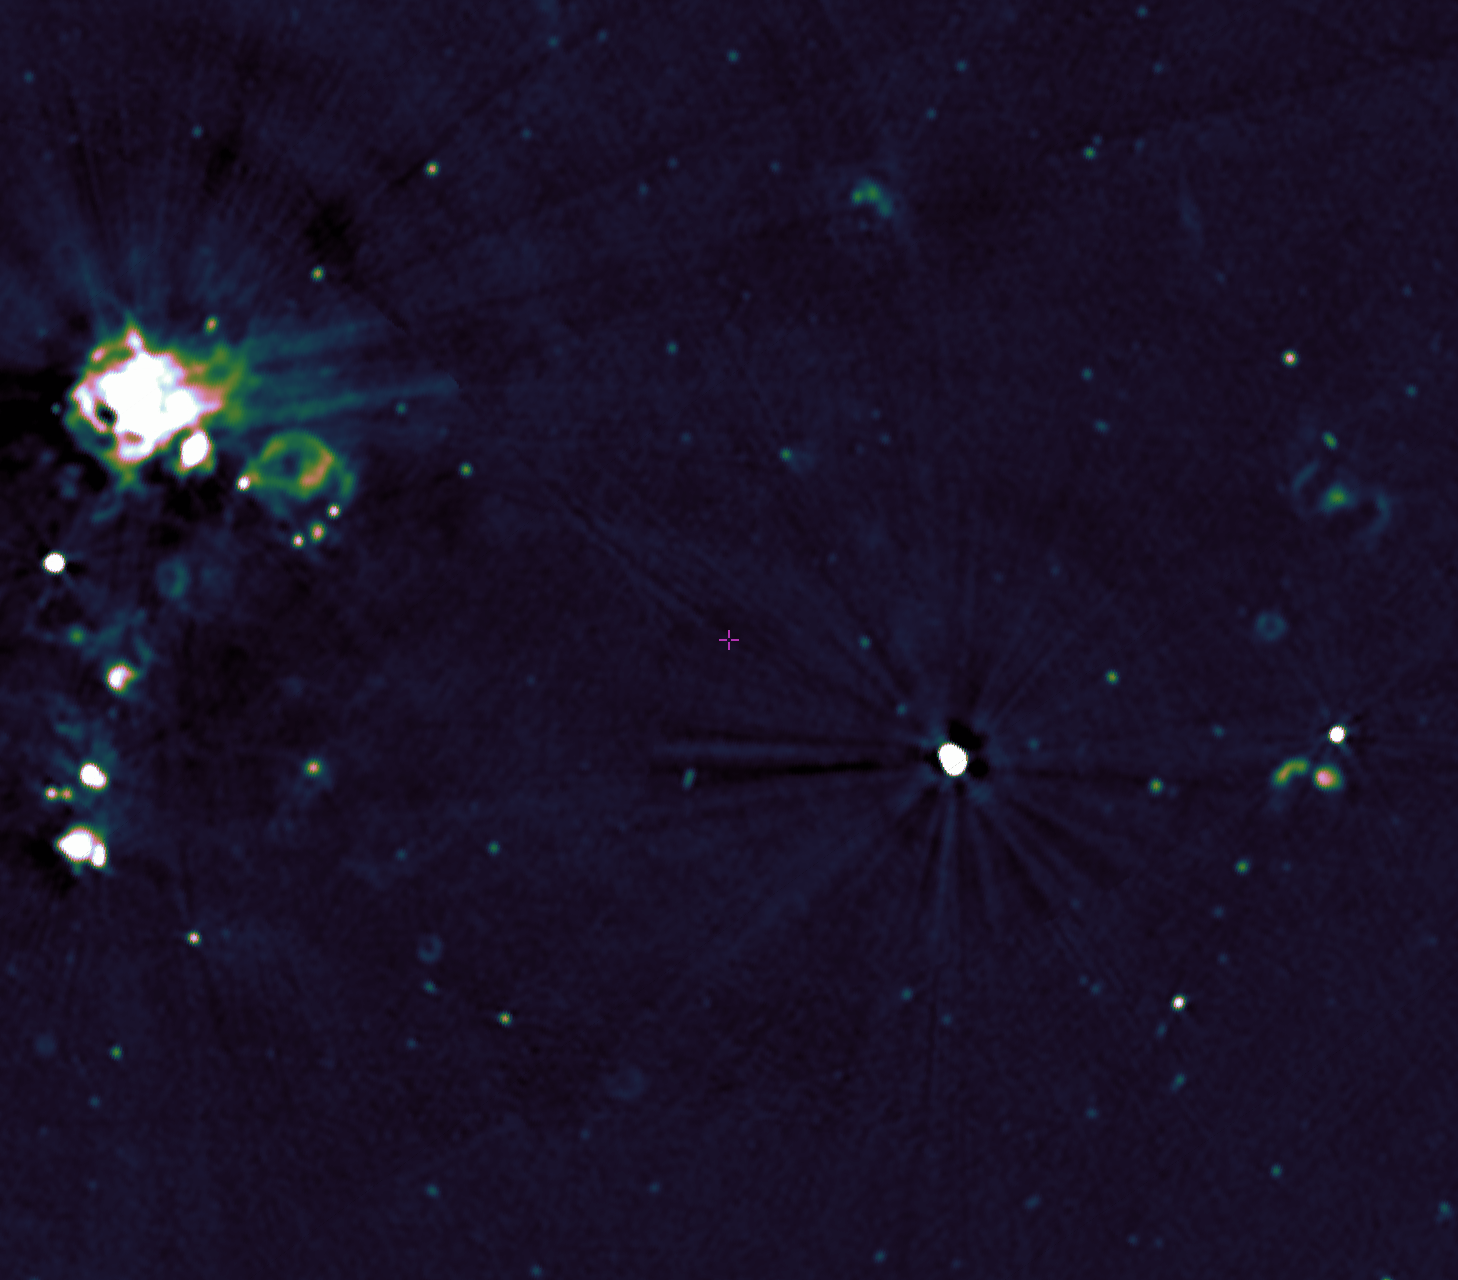
\includegraphics[width=1.0\linewidth]{./chapters/10.results/LMC/radio-843_cut.png}
		\caption{Radio wavelength at 843MHz.}
		\label{results:LMC:radio}
	\end{subfigure}
	\begin{subfigure}[b]{0.375\linewidth}
		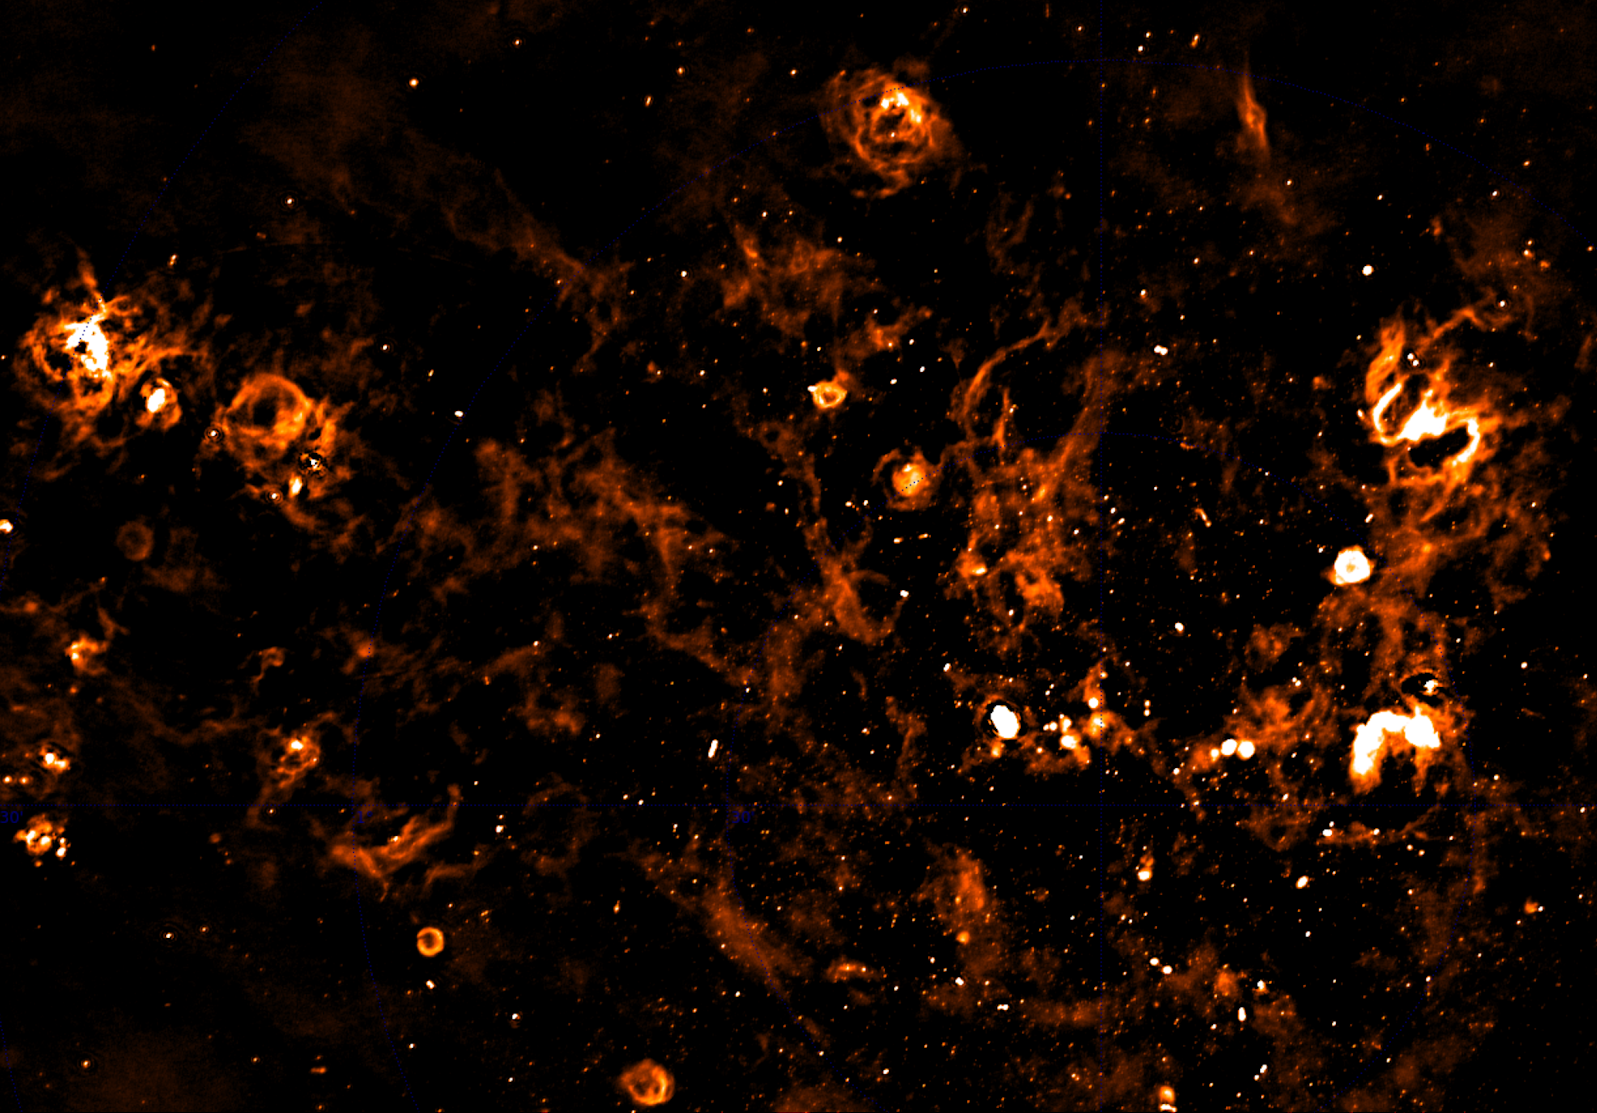
\includegraphics[width=1.0\linewidth]{./chapters/10.results/LMC/meerkat2.png}
		\caption{Wide band radio image by MeerKAT.}
		\label{results:LMC:meerkat}
	\end{subfigure}
	\caption{Section of the Large Magellanic Cloud (LMC)}
	\label{results:LMC}
\end{figure}

The MeerKAT observation covers a wide band of radio frequencies. The lowest frequency in the MeerKAT observation is 894 MHz, and the highest frequency is 1658 Mhz.
Imaging the whole frequency band requires a wide band deconvolution algorithm. In wide band imaging, several images at different frequencies get deconvolved as an image cube. Wide band imaging again multiplies the amount of work that has to be done for reconstruction, as now we cannot deconvolve a single image, but have to deal with a whole image cube.

Wide band imaging is not possible within the time frame of this project. We take a narrow band subset of 5 channels from the original data (ranging from 1084 to 1088 MHz, about 1 Gb in size) for reconstruction. We also reduce the field-of-view to a more manageable section. Figure \ref{results:cutout} shows the LMC image section we are using together with a CLEAN reconstruction of the narrow band data.

\begin{figure}[h]
	\centering
	\begin{subfigure}[b]{0.4\linewidth}
		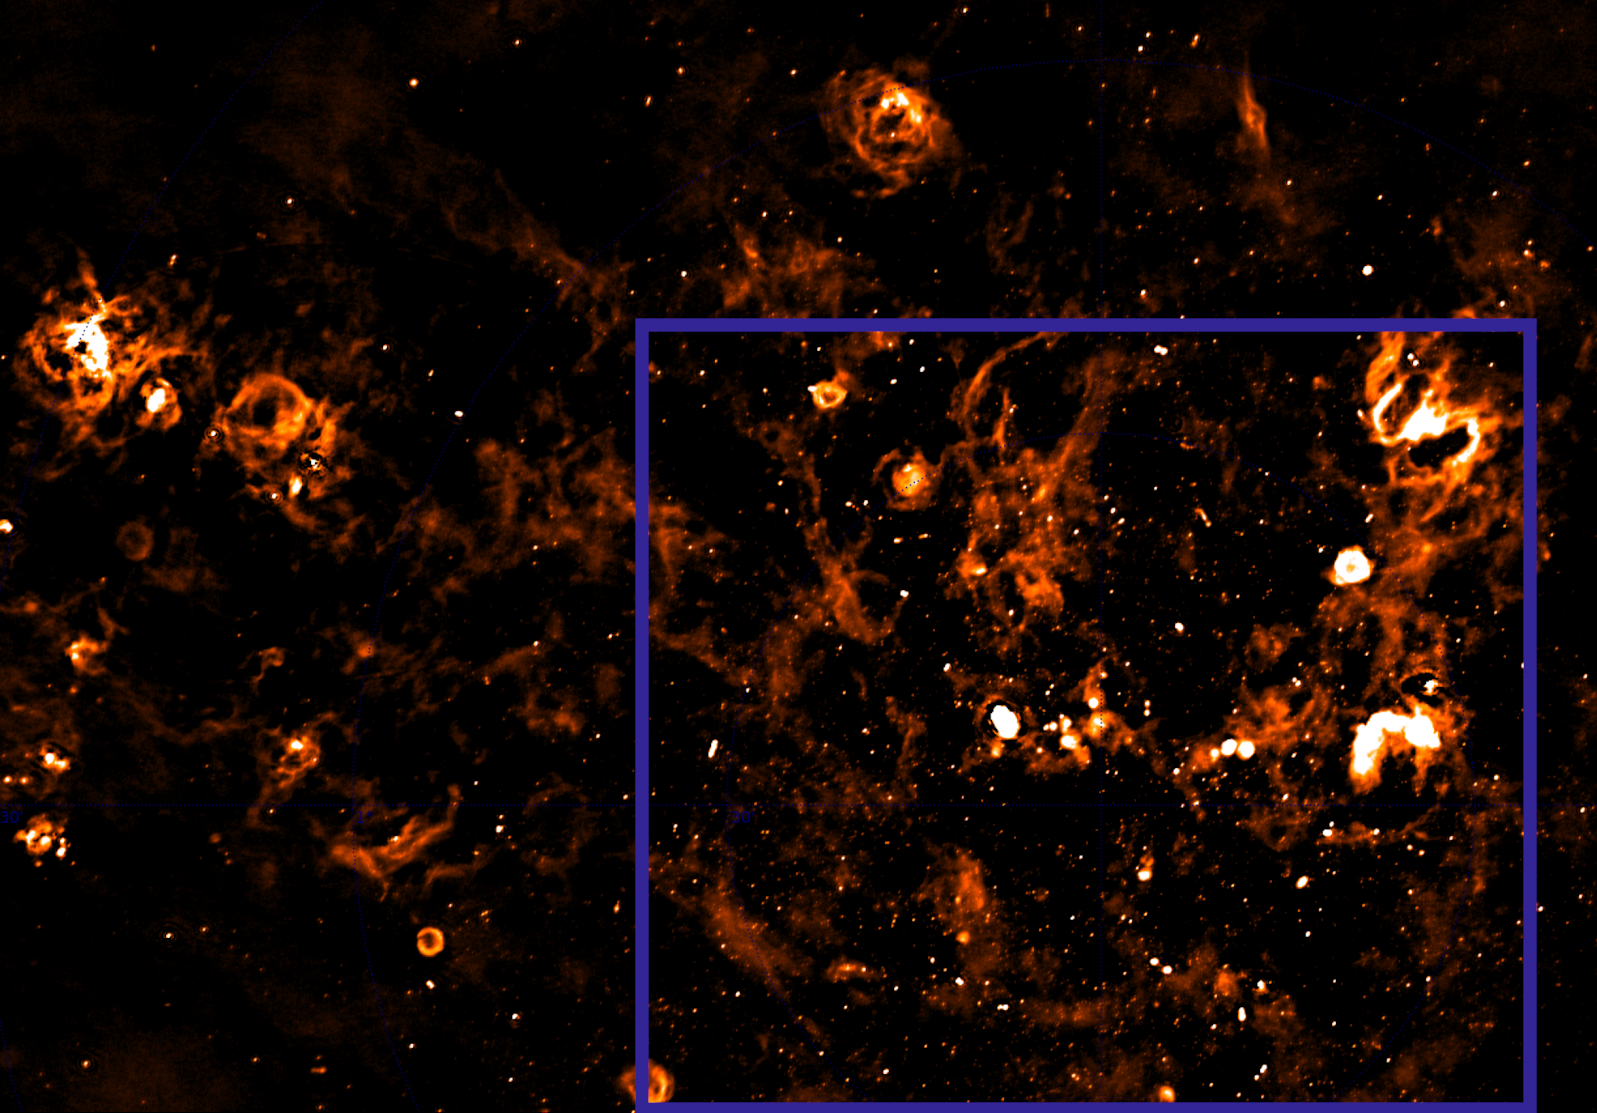
\includegraphics[width=1.0\linewidth]{./chapters/10.results/LMC/meerkat_cutout.png}
	\end{subfigure}
	\begin{subfigure}[b]{0.28\linewidth}
		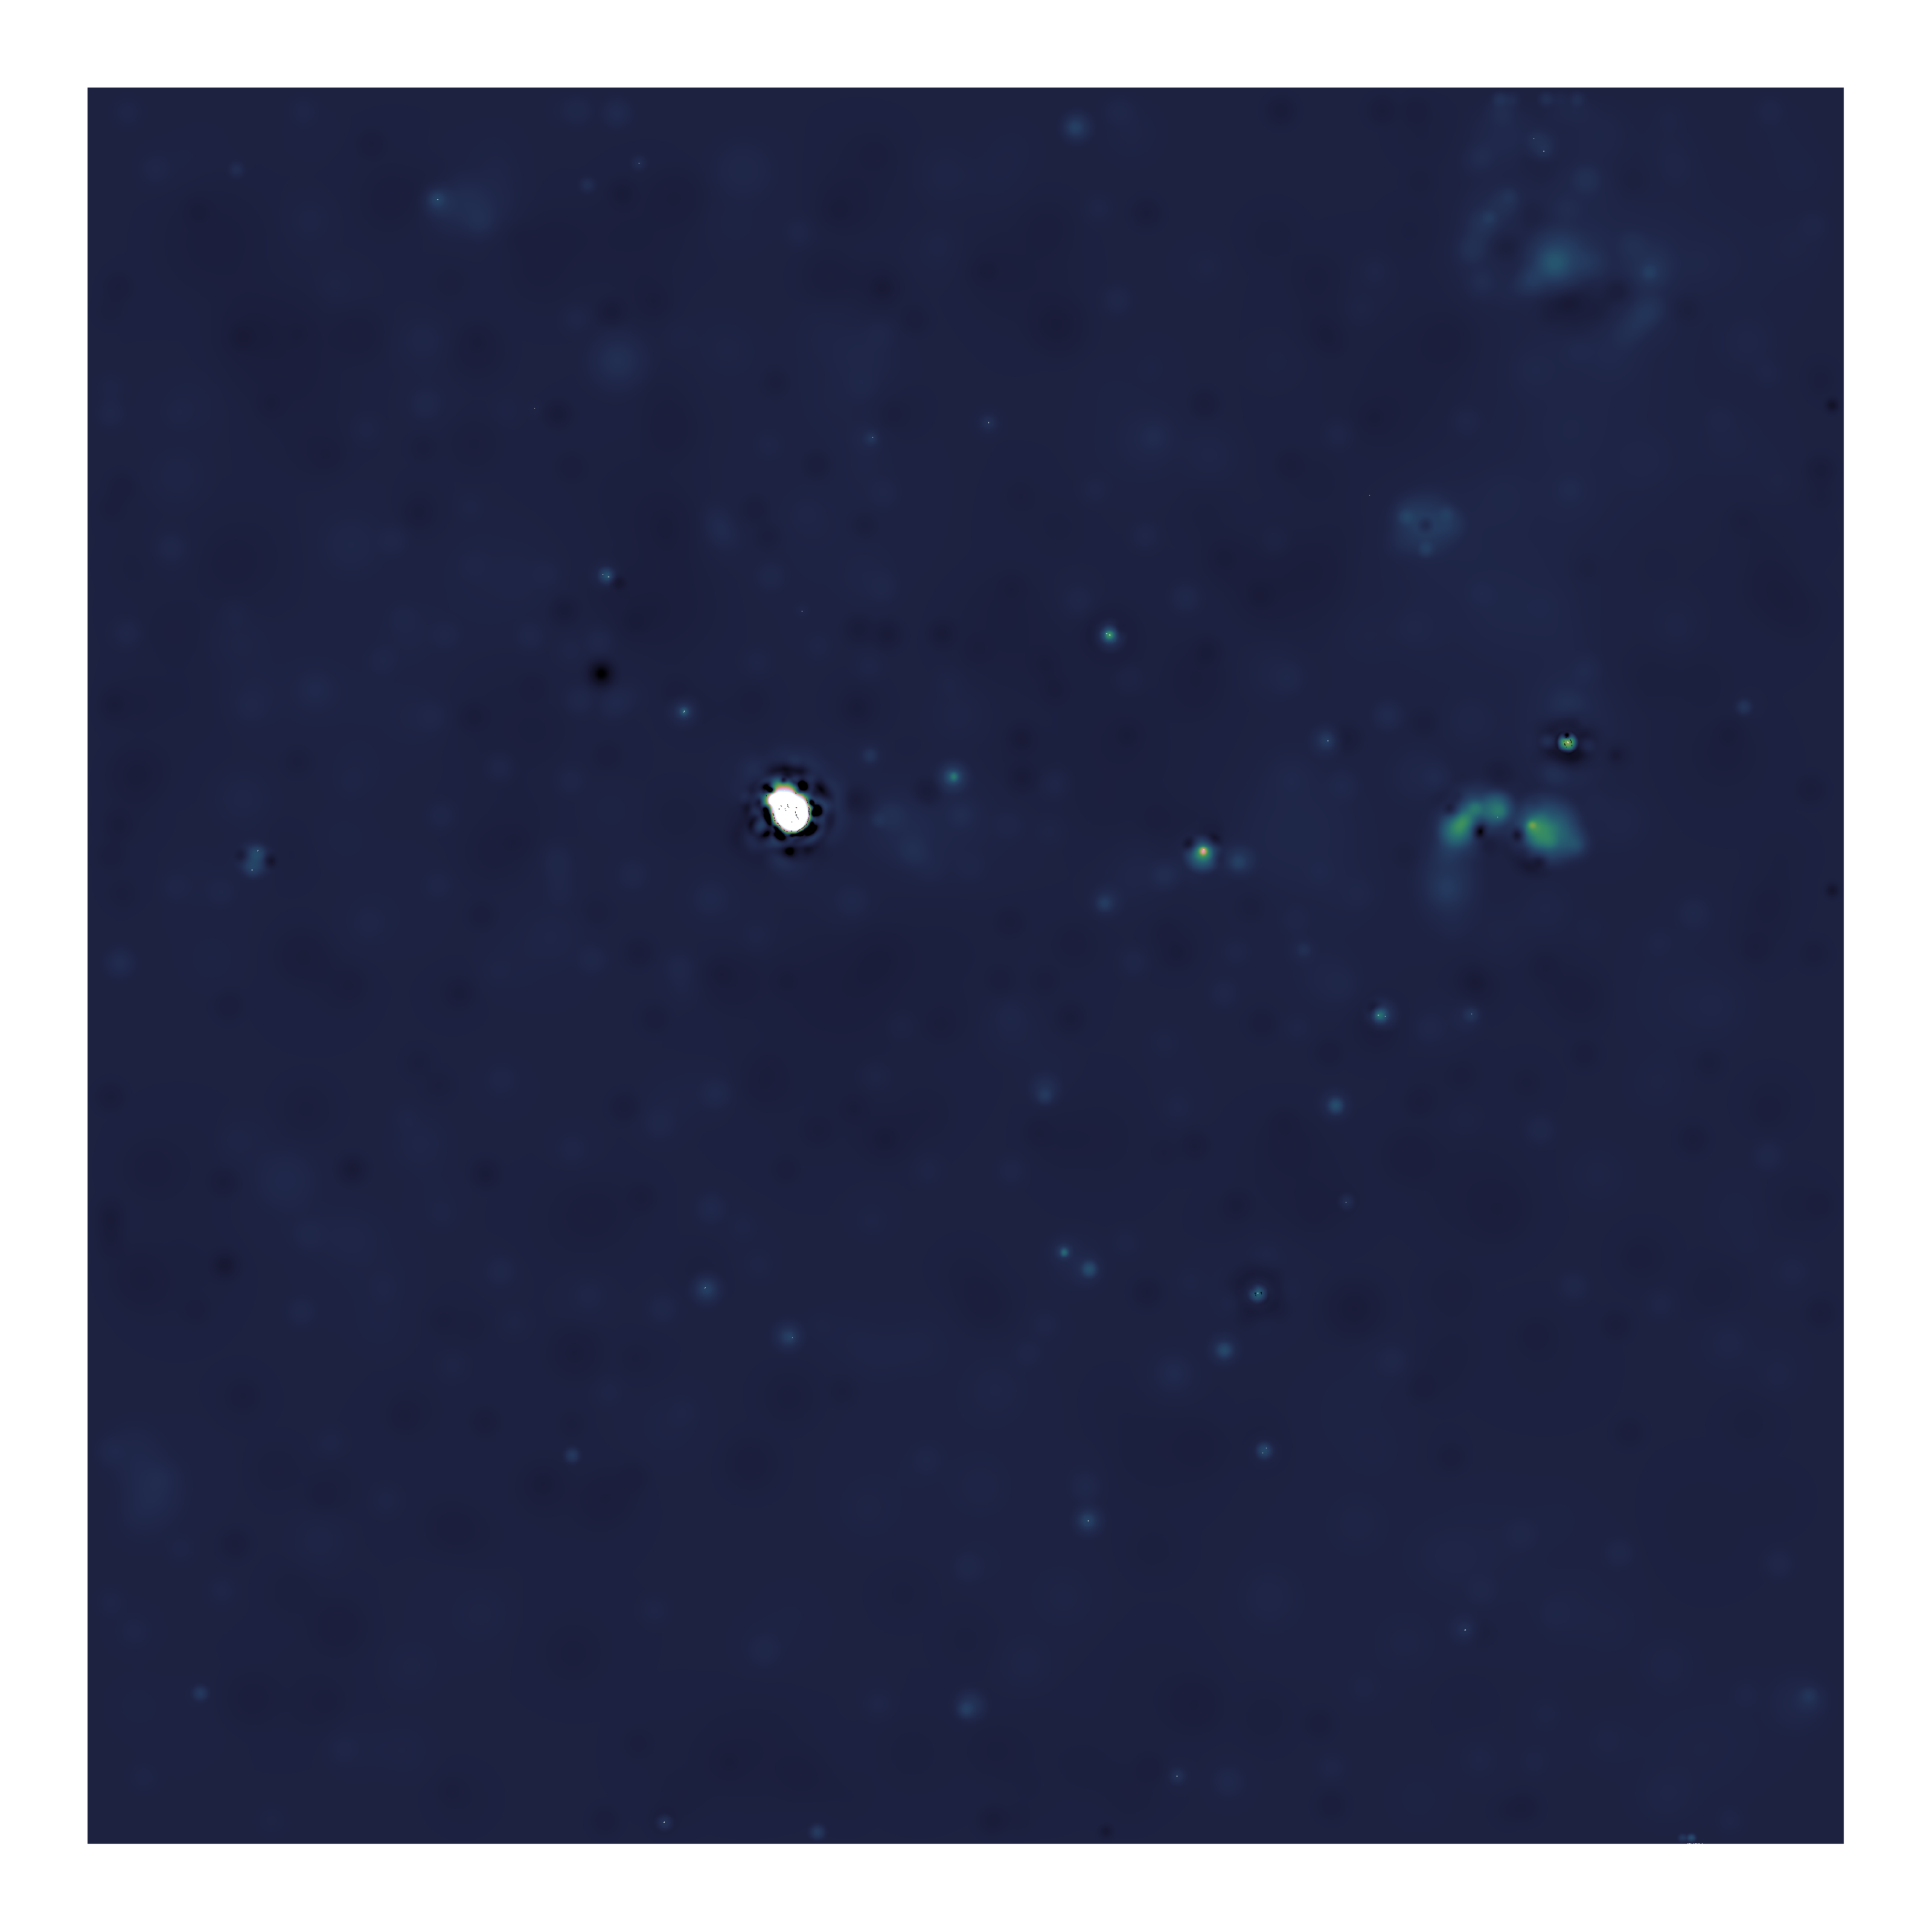
\includegraphics[width=1.0\linewidth, clip, trim={0.72in 0.72in 0.72in 0.72in}]{./chapters/10.results/MSClean/Natural-CLEAN_naked.png}
	\end{subfigure}
	\caption{Narrow band image section used.}
	\label{results:cutout}
\end{figure}

At the center of our image section \ref{results:cutout} we see the N132D supernova remnant. We partially see the faint extended emissions, although they are close to the noise level. This is known as a high-dynamic range reconstruction. We have strong radio sources mixed together with faint emissions, which are only marginally above the noise level of the image.

The total field-of-view of our image section is roughly 1.3 degrees(or $\approx$77 arc minutes). Our reconstruction has $3072^2$ pixel with a resolution of 1.5 arc seconds per pixel. this is still a wide field-of-view reconstruction problem. We have to account for the effects of the $w$-term to achieve a high-dynamic range reconstruction.

In our test reconstruction, we need to account for $w$-term correction and high-dynamic range. We have excluded wide-band imaging as not feasible within the time frame of this project. In Section \ref{results:cleancomp} we compare the reconstructions of CLEAN with our serial coordinate descent algorithm on the LMC observation. The next Section \ref{results:speedup} presents the speedup we achieve with serial coordinate descent by using our distributed or GPU-accelerated implementations.

In Section \ref{results:gradients} we show the core result of this project. Namely what effect an approximate $PSF$ has on the deconvolution problem and whether we can use it to further distribute the problem. The answer to that question is affirmative: We can approximate the $PSF$, and we can exploit it to further distribute the deconvolution. But we need more sophisticated coordinate descent algorithms to fully benefit from it.


\subsection{Comparison with state-of-the-art reconstruction algorithms} \label{results:cleancomp}
We compare our serial coordinate descent algorithm with the state-of-the-art algorithms multi-scale CLEAN and MORESANE on the LMC data set. We test against the WSCLEAN \cite{offringa2014wsclean} implementation of multi-scale CLEAN and MORESANE (IUWT)\footnote{The WSCLEAN package has a re-implementation of the original MORESANE algorithm\cite{dabbech2015moresane}, which is called IUWT.}, and compare the resulting model and restored images. The model image is the direct output of the deconvolution algorithm. The restored image is convolved with the 'clean-beam', a 2D Gaussian function representing the instrument's accuracy\footnote{Usually, the residuals are added to the restored image. We compare the restored images without the added residuals.}. A reconstruction algorithm achieves super-resolution, if the model image it produces contains plausible structures.

We first compare the model and the residual images of the three algorithms. The reconstruction algorithm should detect all sources (we have a non-zero pixels for all point- and extended sources) and leave as little of the true emissions in the residuals as possible. Meaning we should not see any remaining structures of the image \ref{results:cutout} in the residuals. Figure \ref{results:cleancomp:figure} shows the model- and residual image of multi-scale CLEAN, serial coordinate descent and MORESANE.

\newpage

\begin{figure}[!htp]
	\centering
	\begin{subfigure}[b]{0.82\linewidth}
		\centering
		\begin{subfigure}{0.49\linewidth}
			\centering
			\textbf{Model image}
			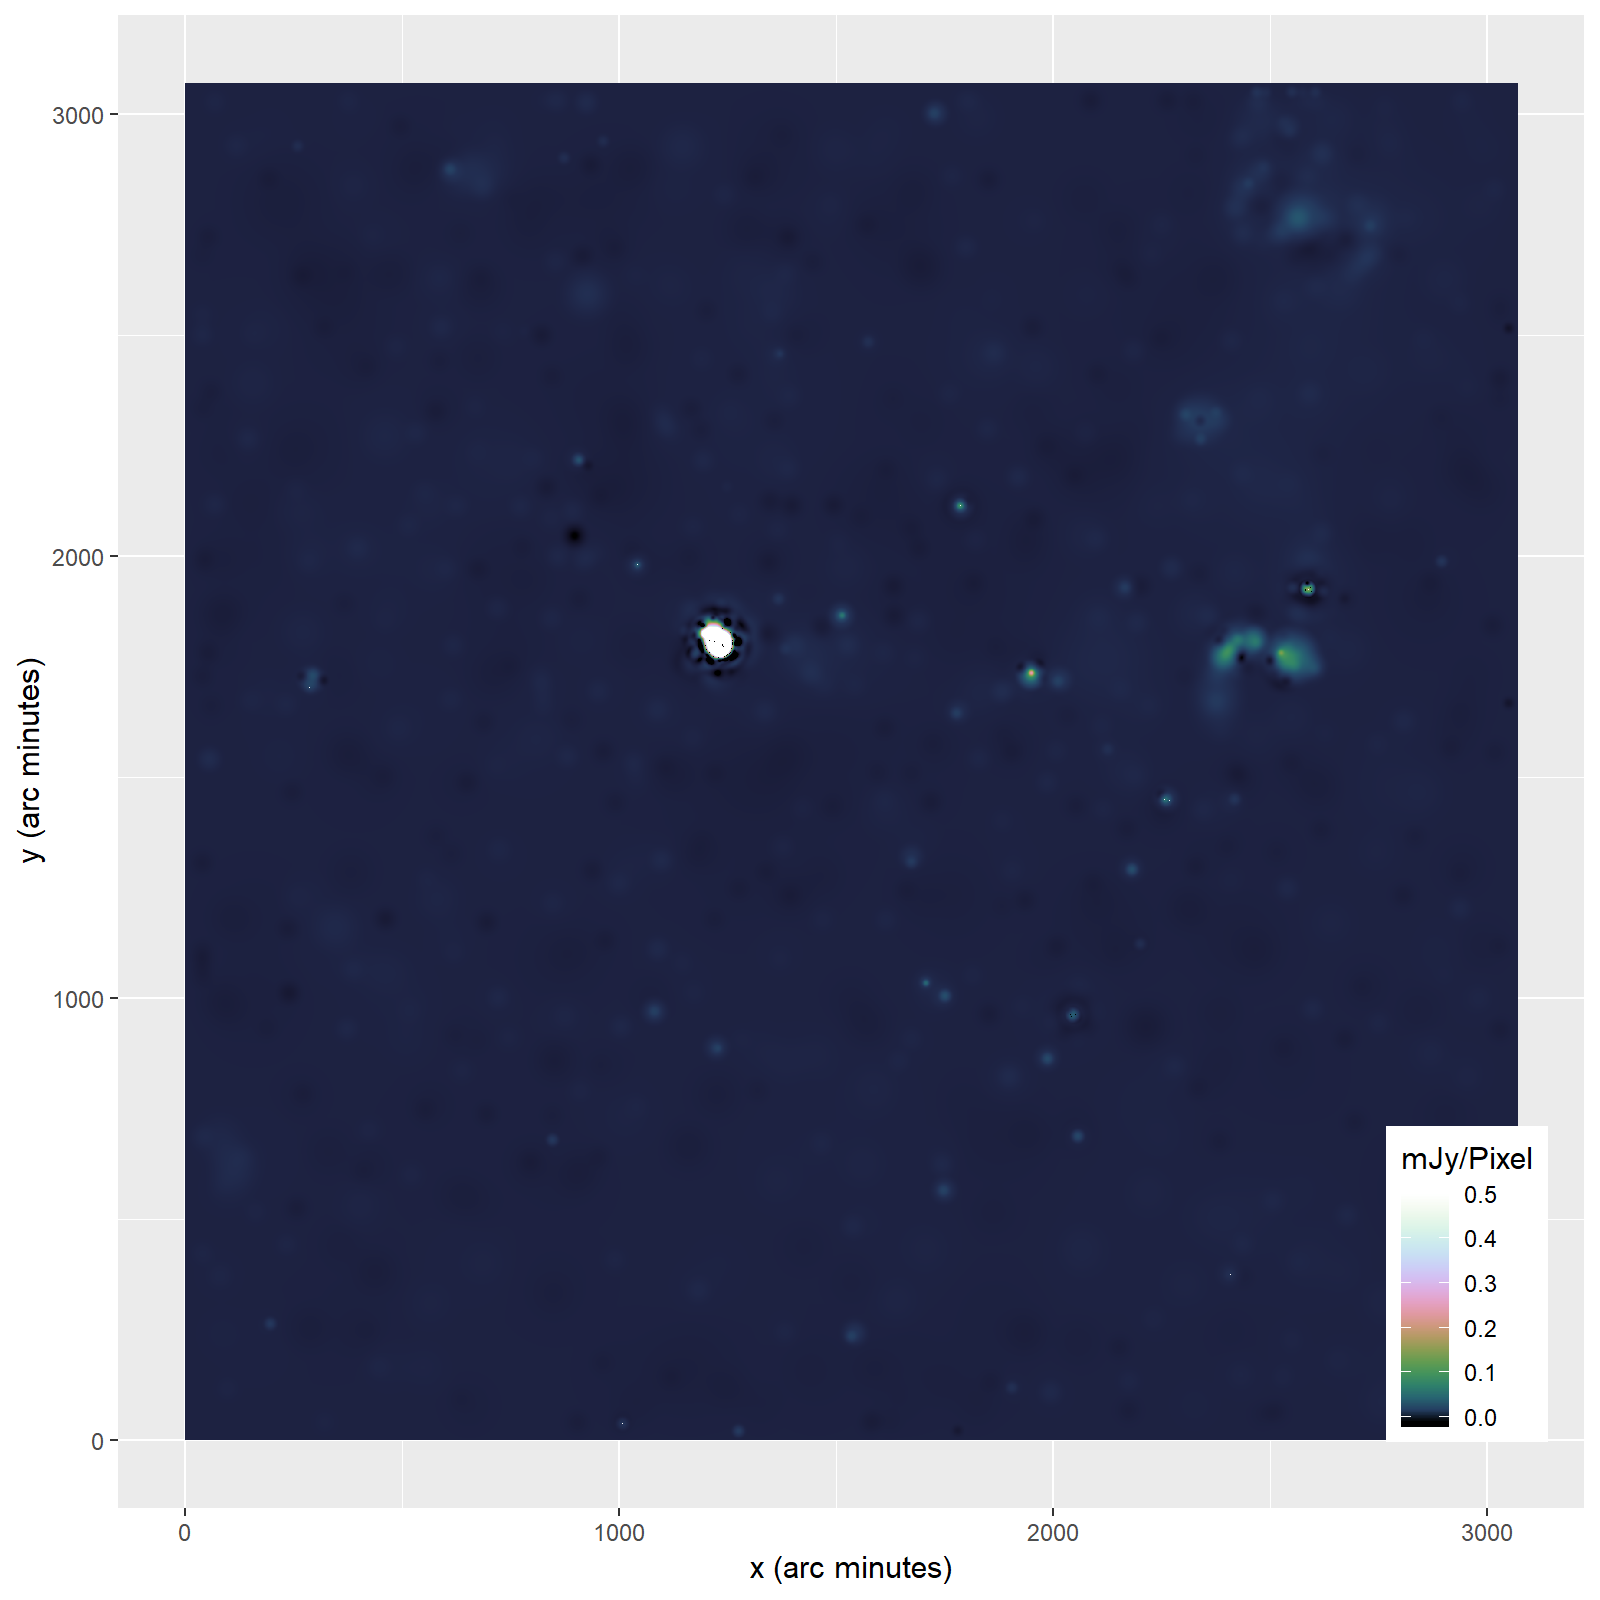
\includegraphics[width=1.0\linewidth]{./chapters/10.results/MSClean/Natural-CLEAN.png}
		\end{subfigure}
		\begin{subfigure}{0.49\linewidth}
			\centering
			\textbf{Residual image}
			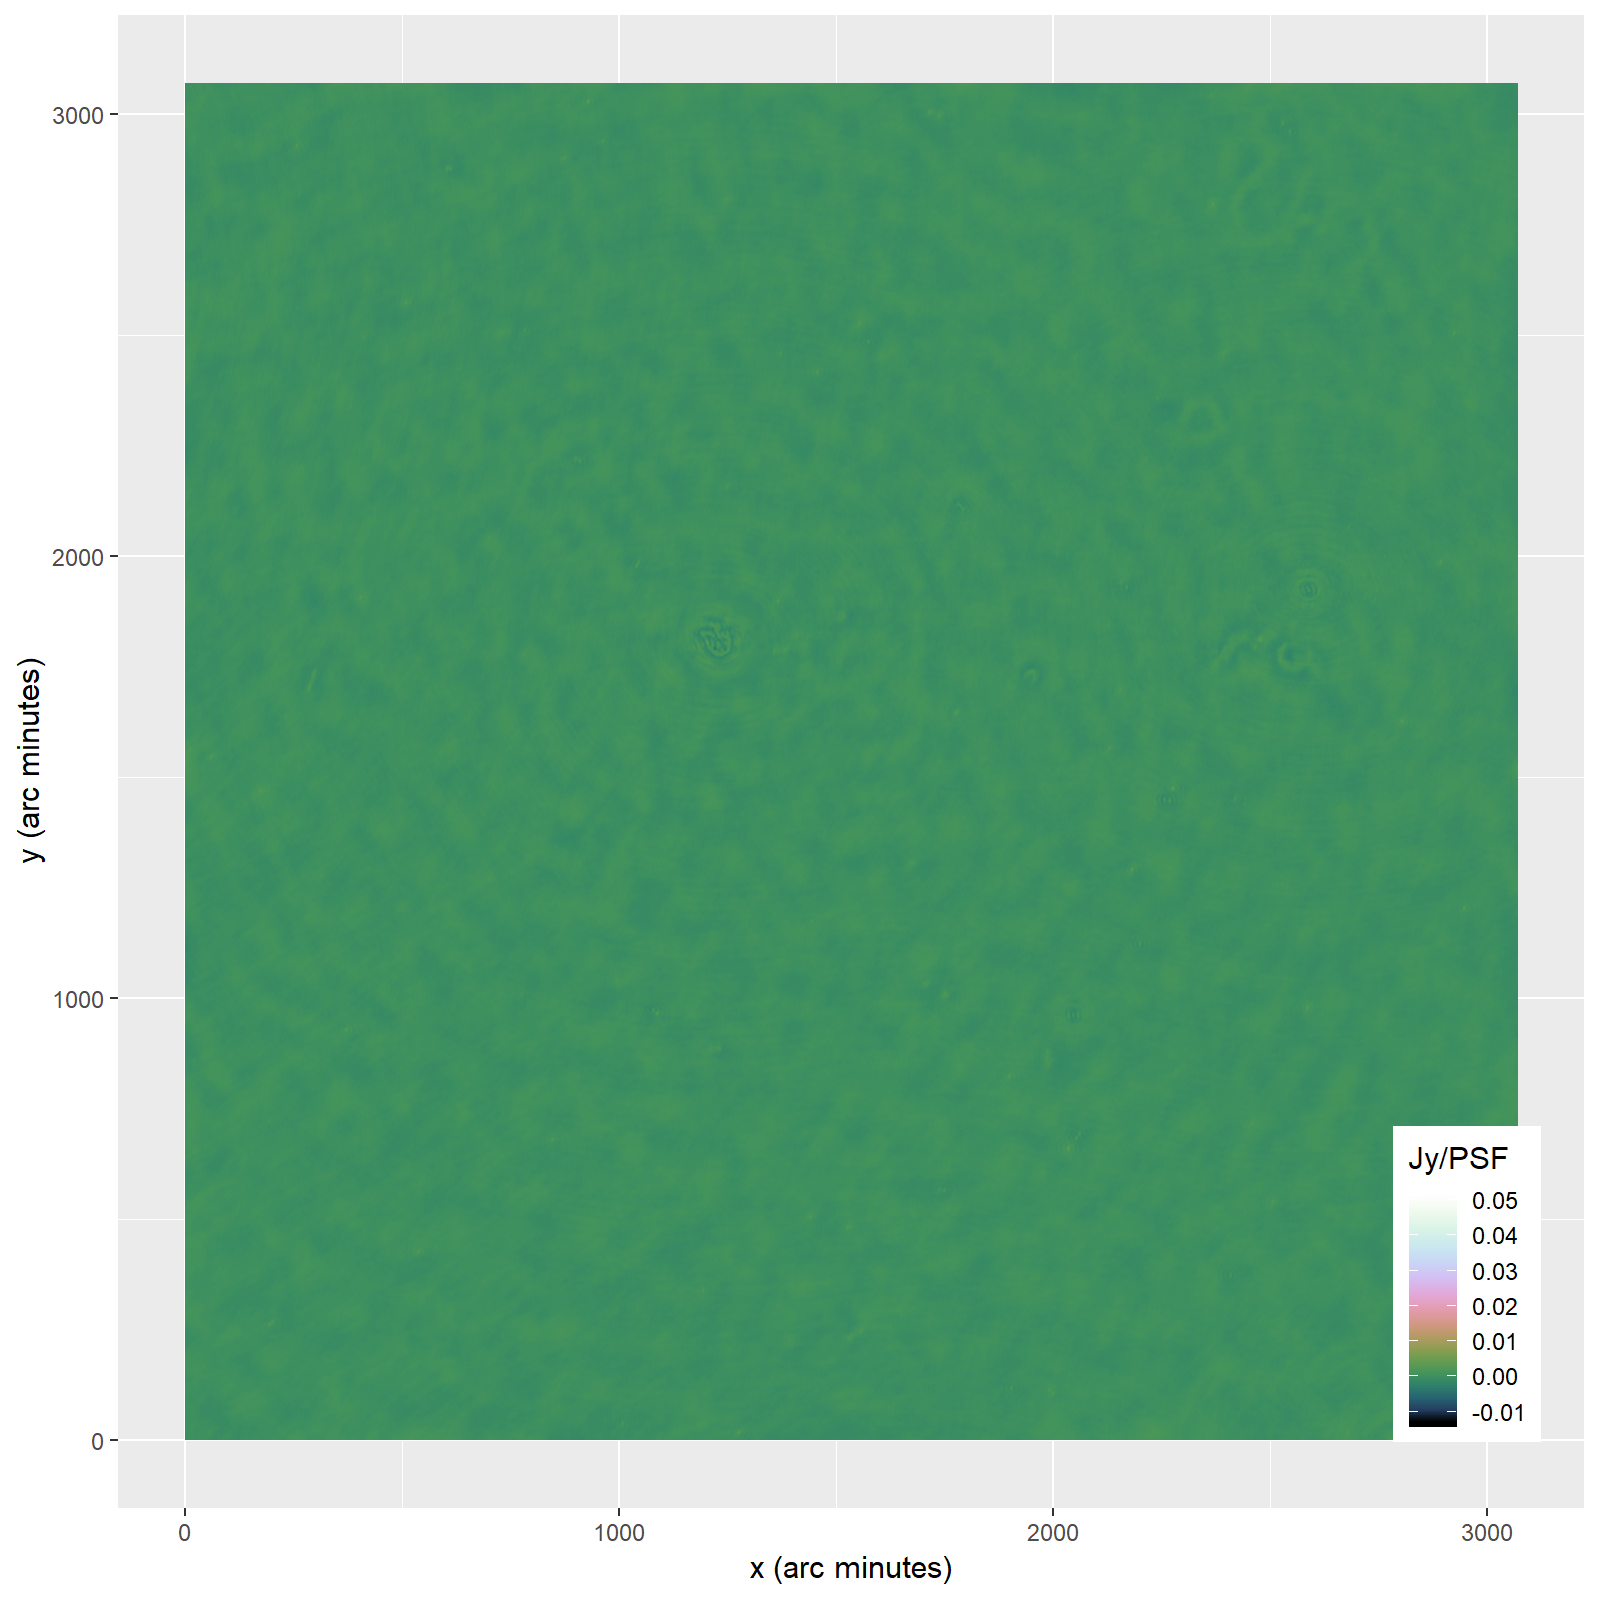
\includegraphics[width=1.0\linewidth]{./chapters/10.results/MSClean/Natural-CLEAN-residuals.png}
		\end{subfigure}
		\caption{Multi-scale CLEAN.}
		\label{results:comp:clean}
	\end{subfigure}
	\begin{subfigure}[b]{0.82\linewidth}
		\centering
		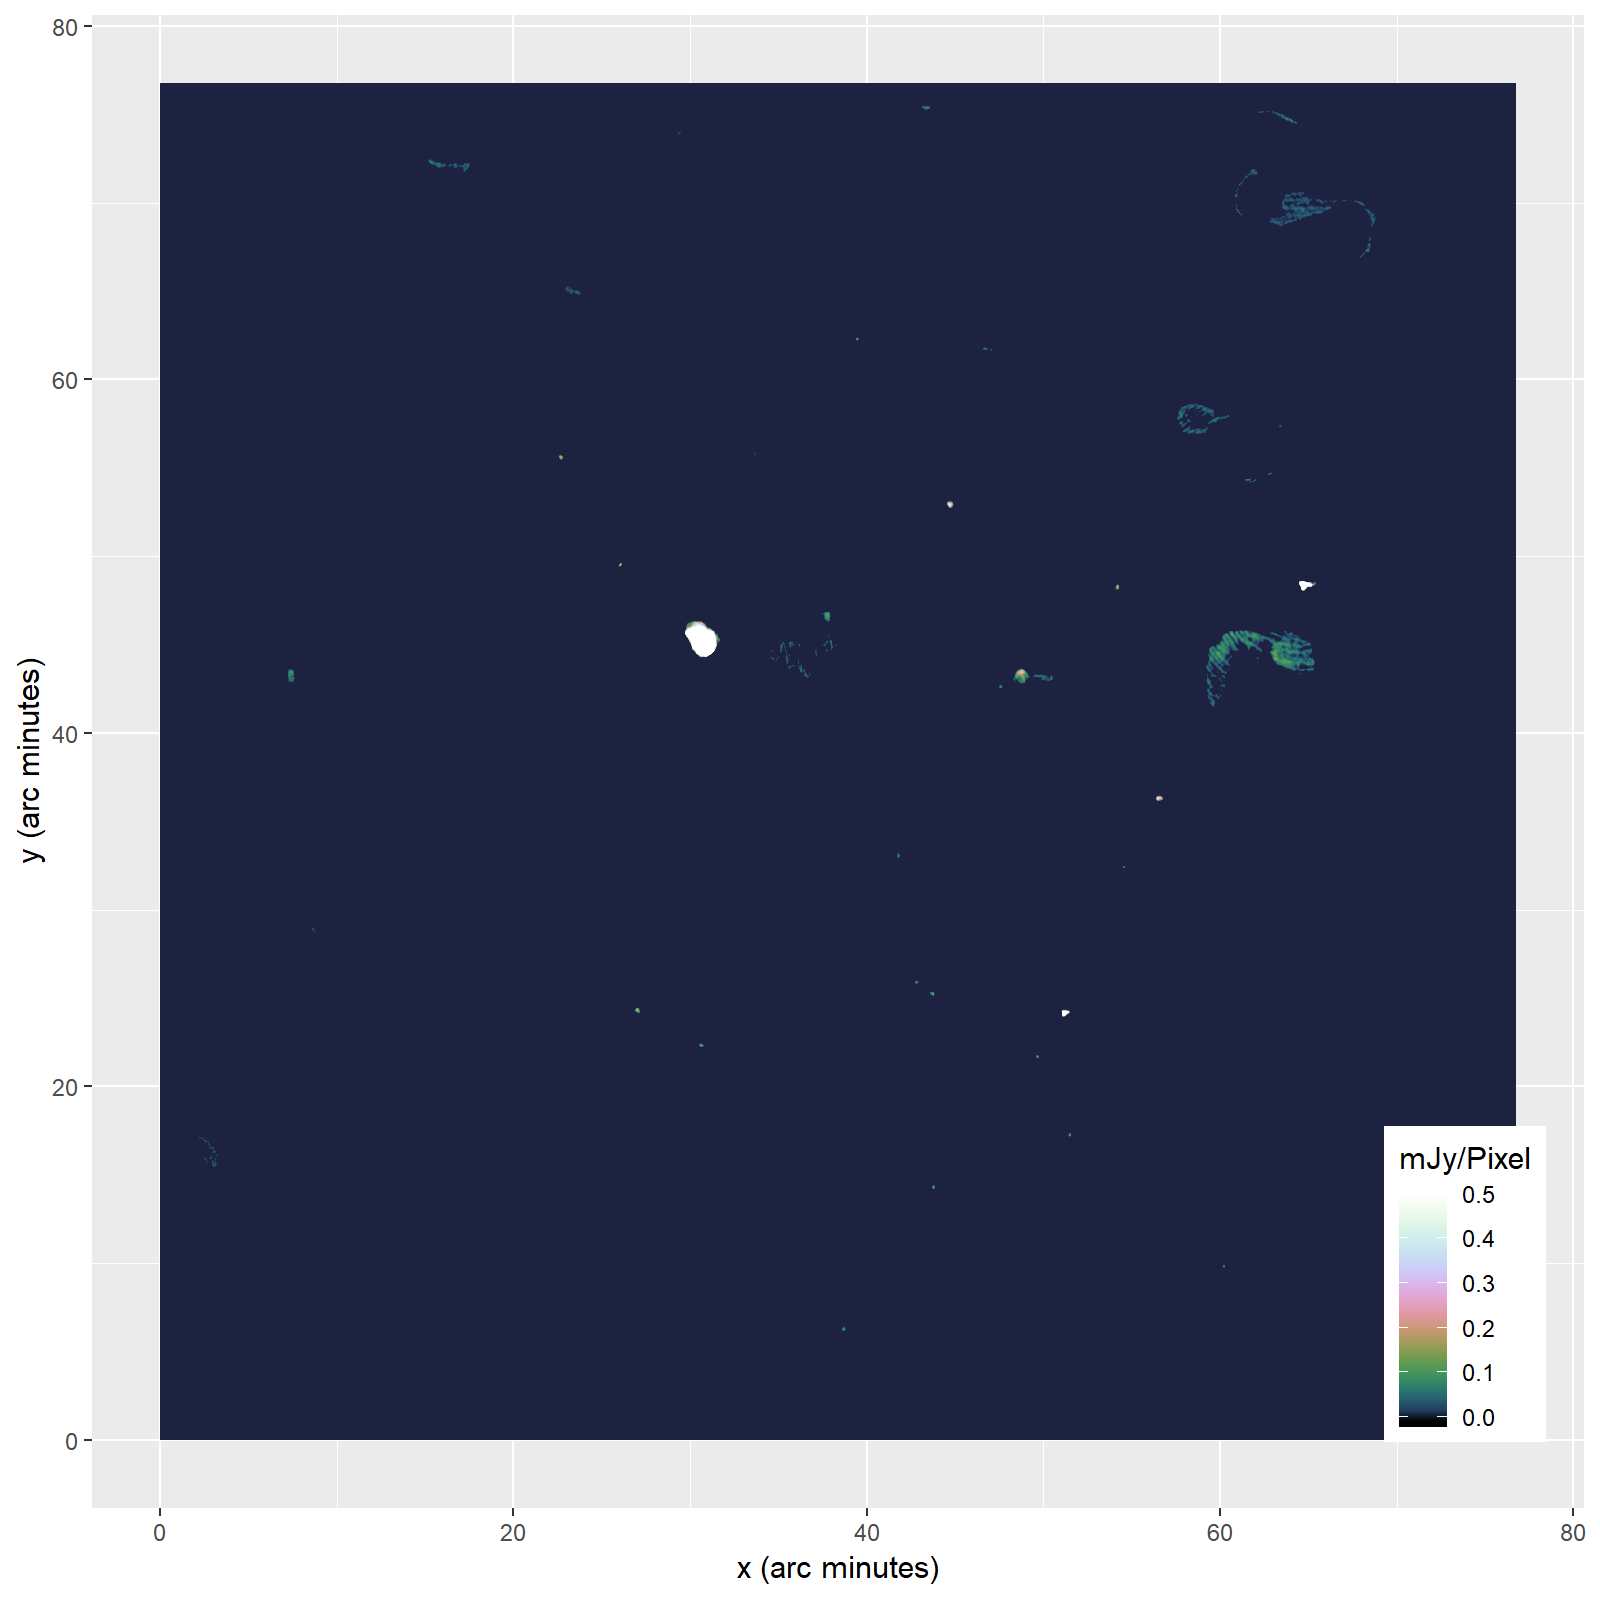
\includegraphics[width=0.490\linewidth]{./chapters/10.results/SerialCD/CD-reference.png}
		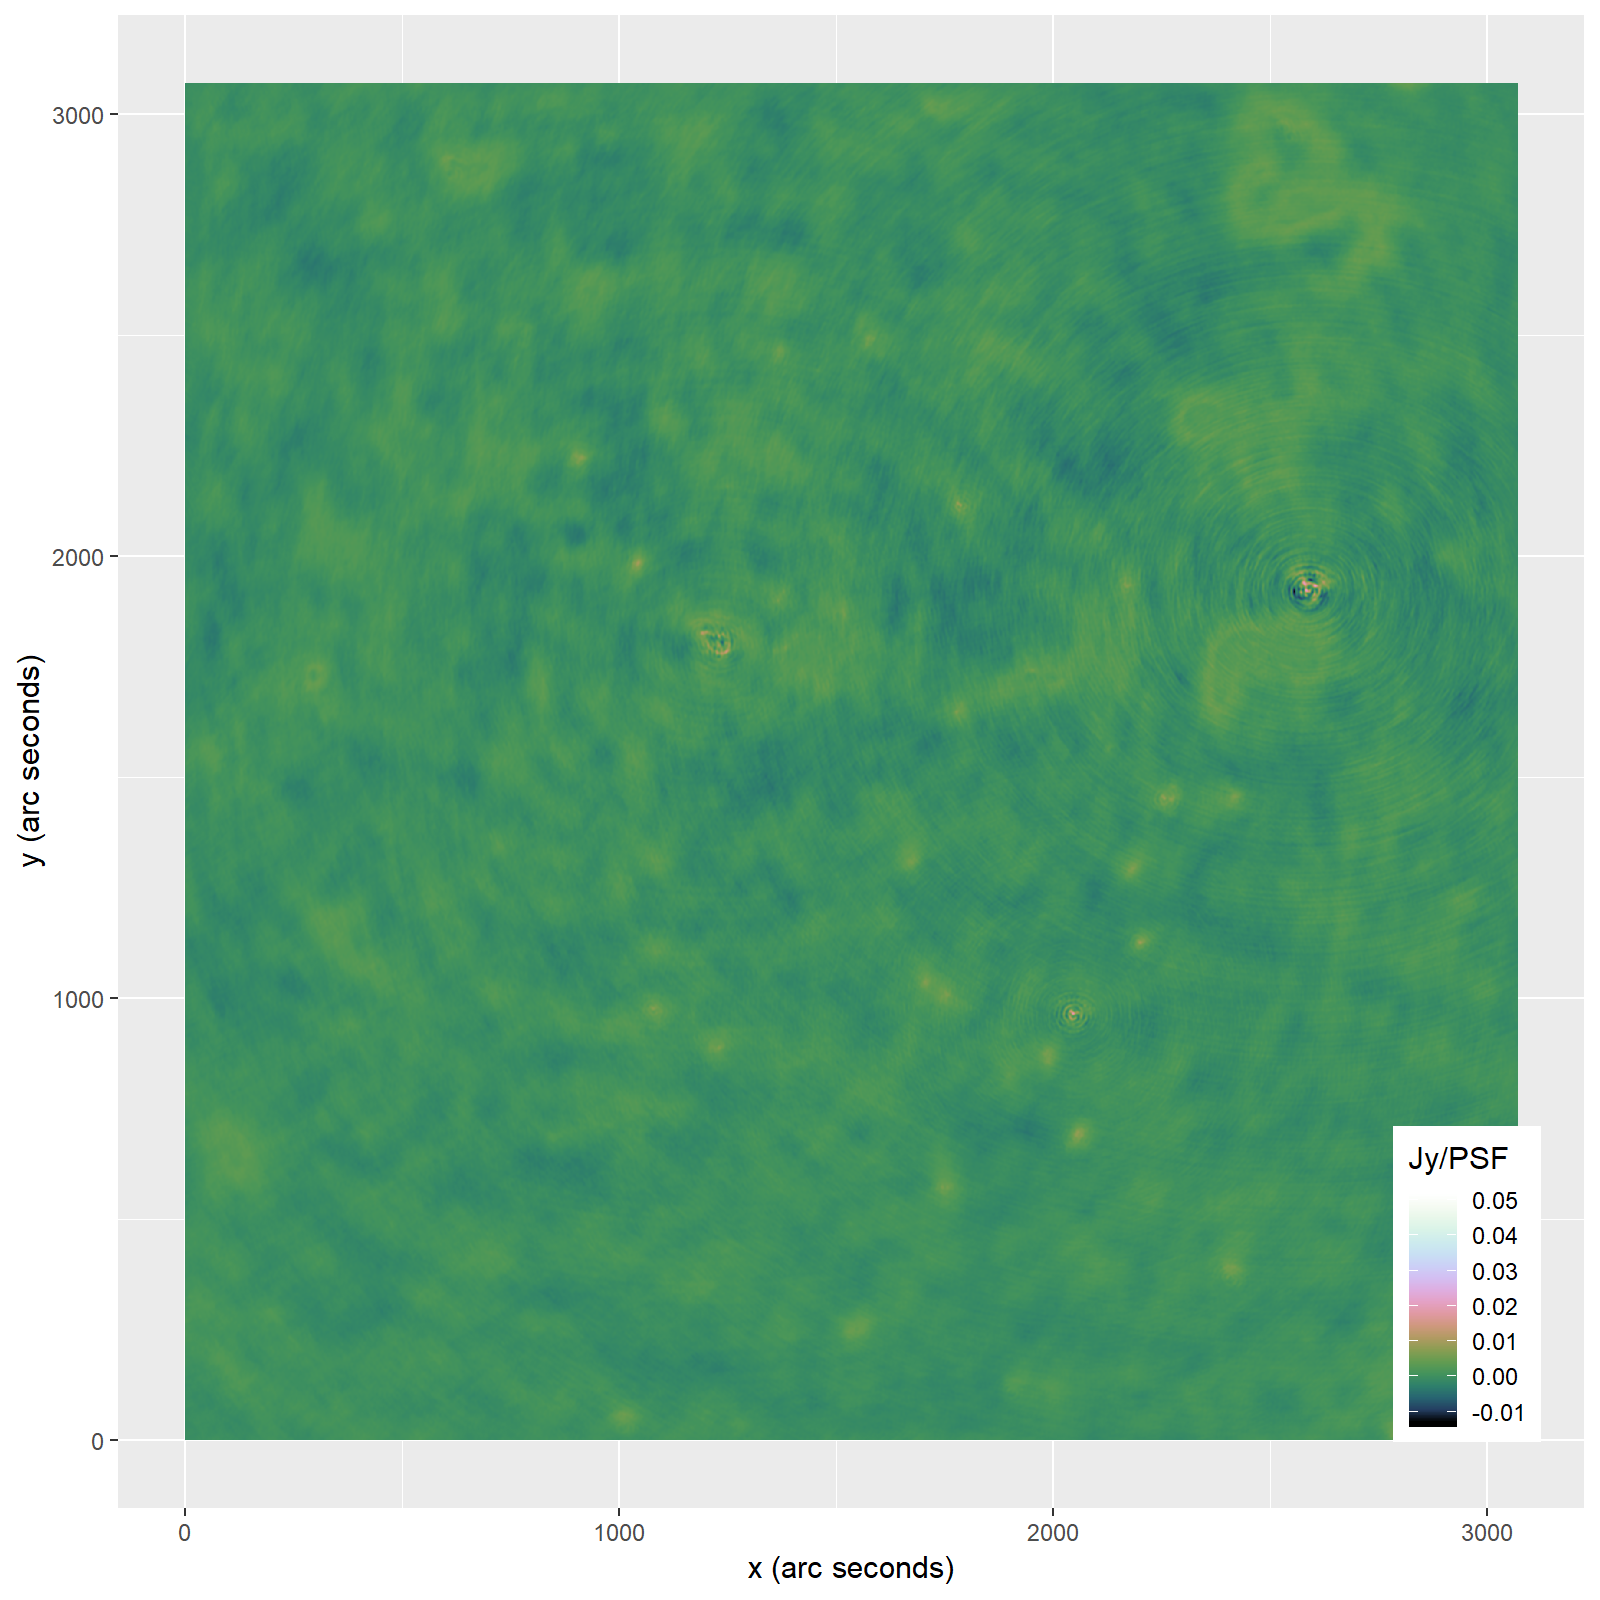
\includegraphics[width=0.490\linewidth]{./chapters/10.results/SerialCD/CD-reference-residuals.png}
		\caption{Coordinate descent with elastic net.}
		\label{results:comp:clean}
	\end{subfigure}
	\begin{subfigure}[b]{0.82\linewidth}
		\centering
		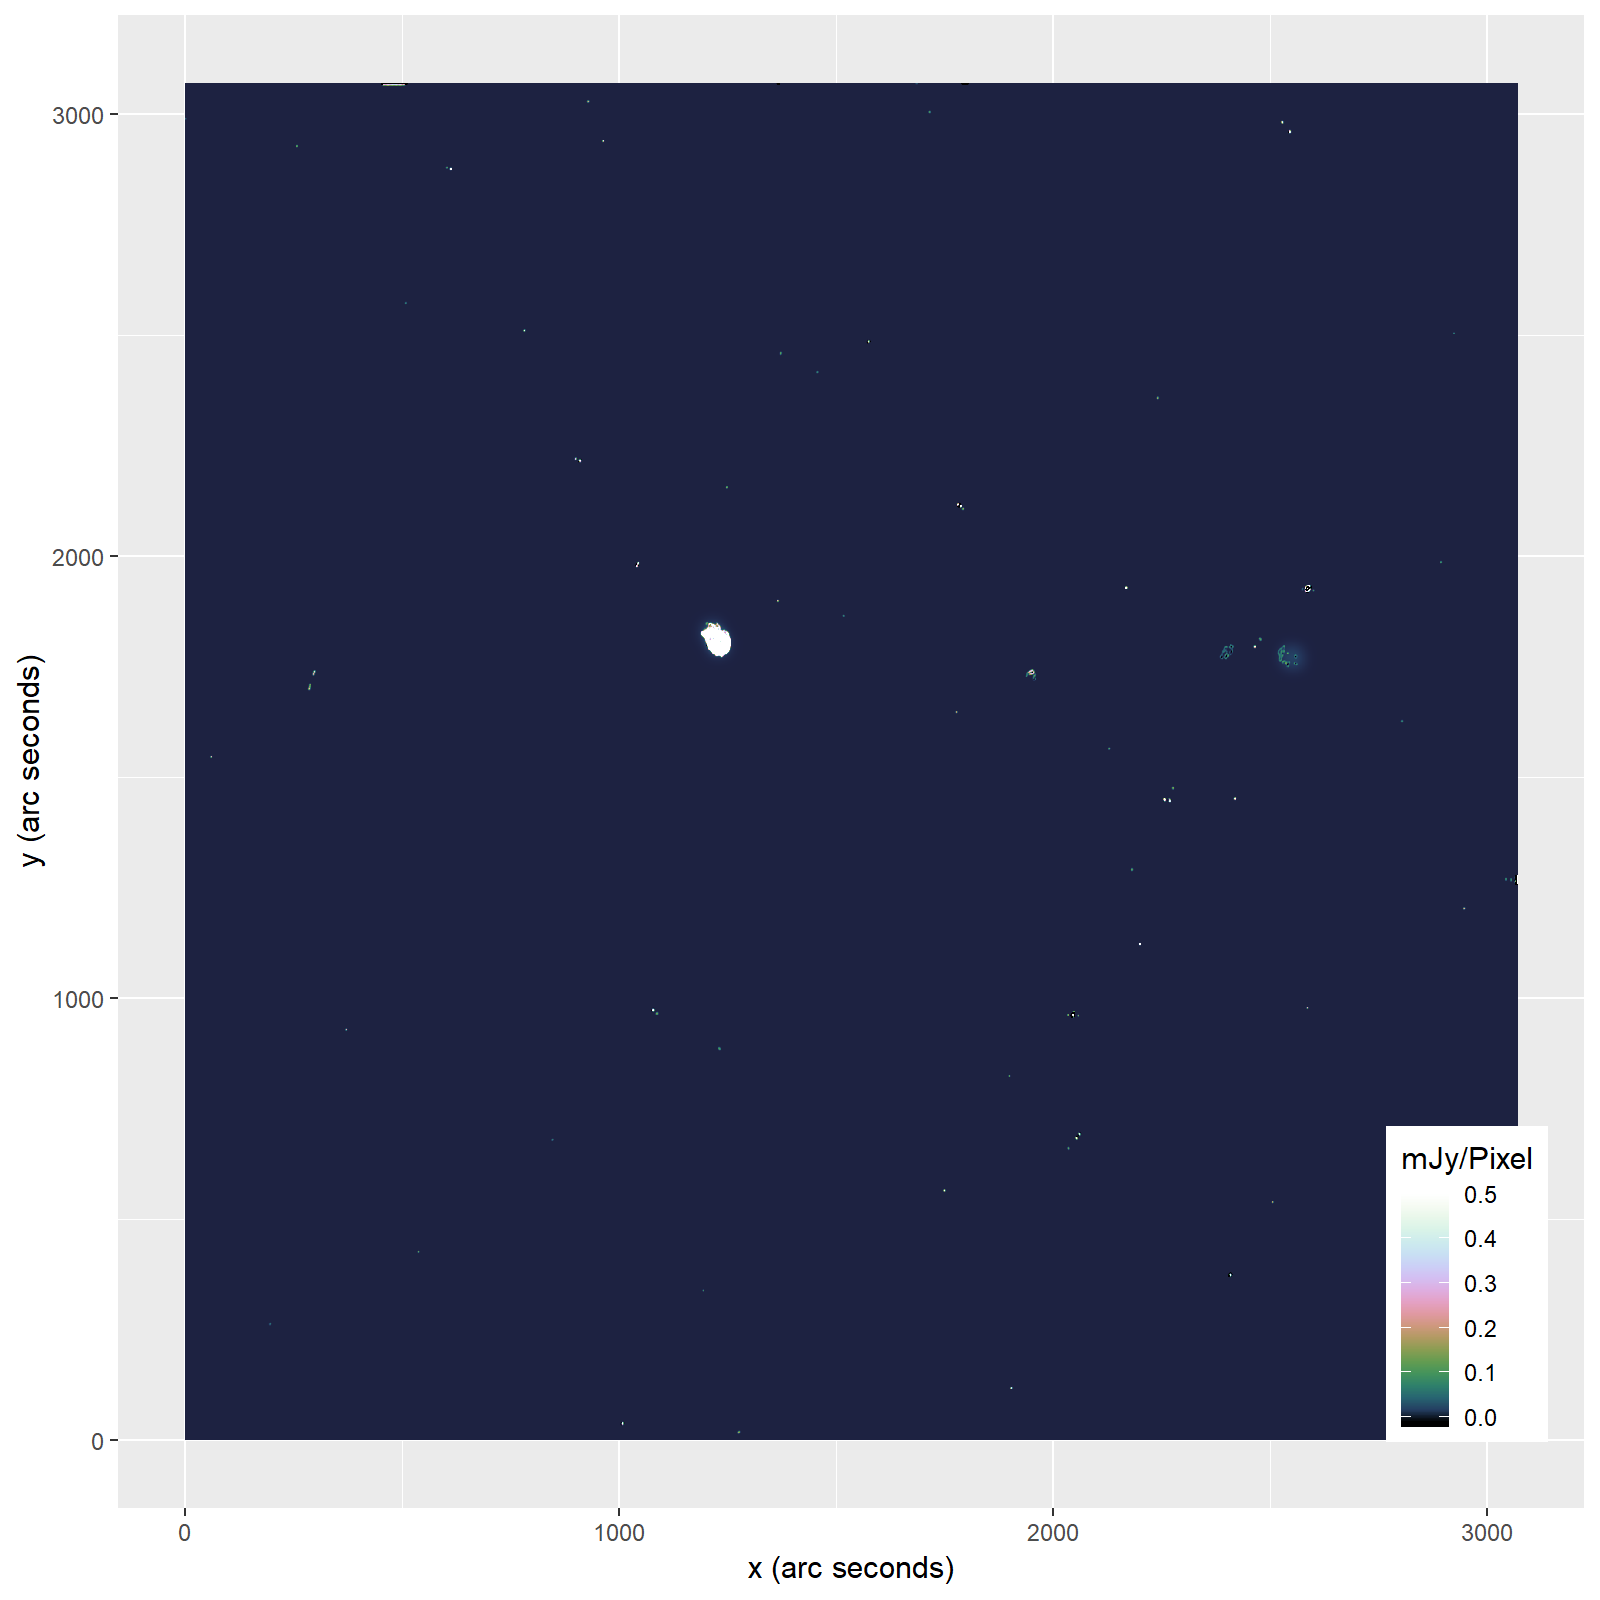
\includegraphics[width=0.490\linewidth]{./chapters/10.results/iuwt/iuwt-model.png}
		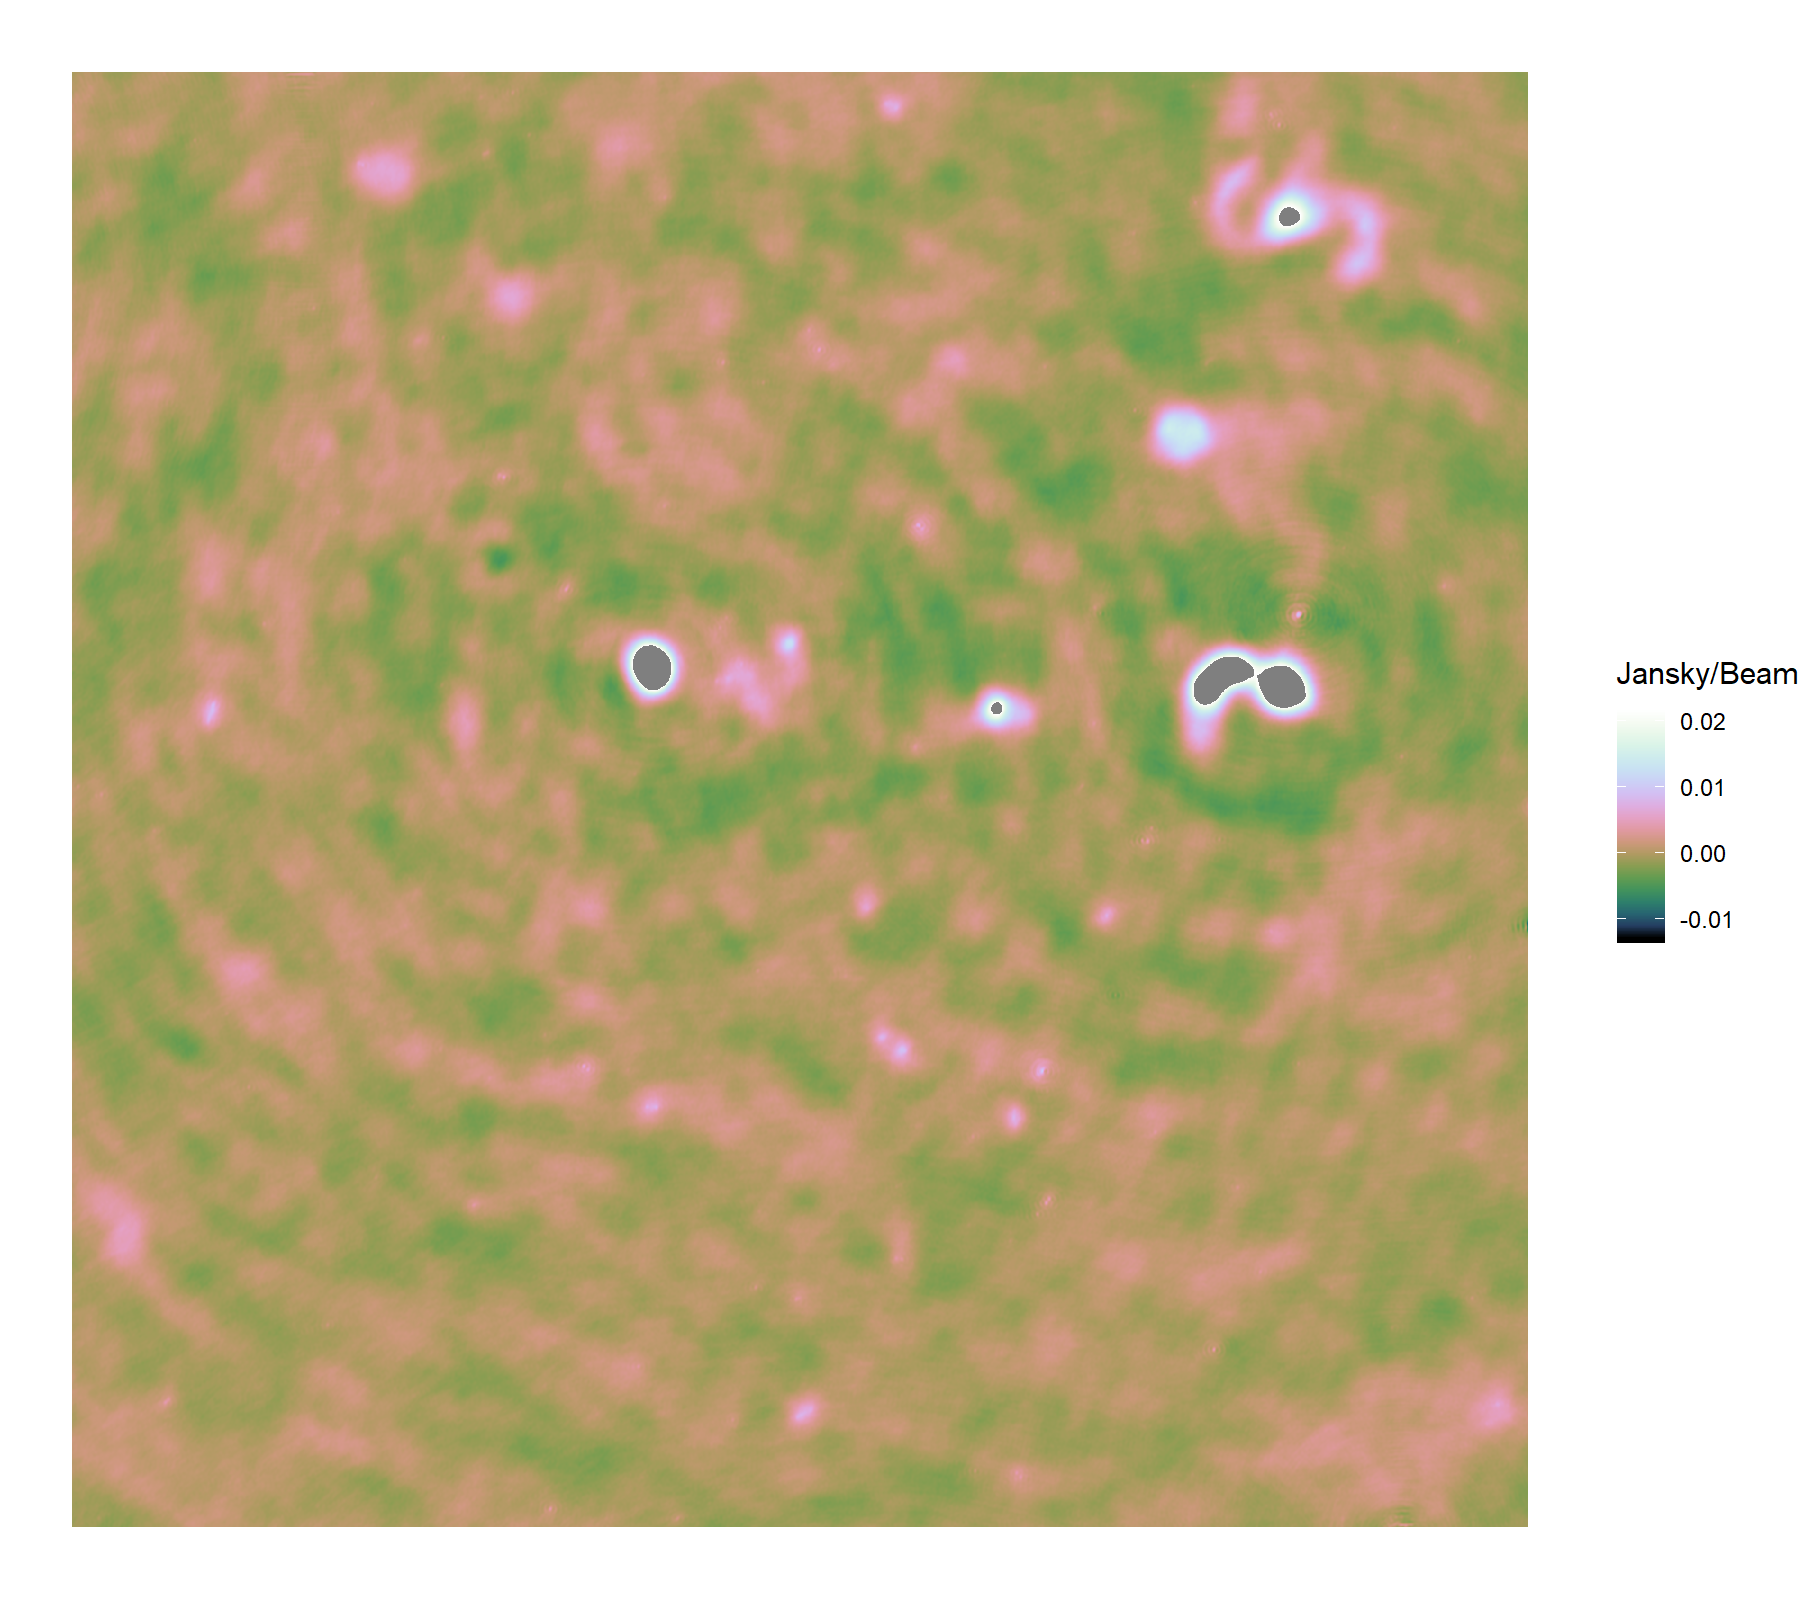
\includegraphics[width=0.490\linewidth]{./chapters/10.results/iuwt/iuwt-residuals.png}
		\caption{MORESANE (IUWT).}
		\label{results:comp:clean}
	\end{subfigure}

	\caption{Comparison of the whole image}
	\label{results:cleancomp:figure}
\end{figure}

\newpage

Multi-scale CLEAN detects all extended emissions (we have non-zero pixels in the model for every source). It has the smallest residual magnitudes of the three algorithms, and has barely visible structures left in the residual image. Multi-scale CLEAN has reconstructed the image close to the noise level. The serial coordinate descent reconstruction does not contain any non-zero pixels in the model image, but its residual image contains still visible structures. The MORESANE reconstruction surprisingly has the largest magnitudes in the residual image. It still has clear structures belonging to the extended sources in the residuals. Also note that MORESANE has not detected the top-right extended emission. It is missing in the model image.

The WSCLEAN software package has implemented an auto-masking strategy for multi-scale CLEAN and MORESANE, which helps the deconvolution algorithm reconstruct an image close to the noise level. At a certain point in the deconvolution, the 'mask' forbids the algorithm to add new sources to the model image. It can only change existing sources to explain the emission left in the residual image. This helps the deconvolution algorithm to reconstruct closer to the noise level, since it is forbidden to add new structures likely to be due to noise. 

The MORESANE algorithm left notable emissions in the residual image. The serial coordinate descent algorithm with elastic net regularization does not use an auto-masking strategy. Nevertheless, its residual image has lower magnitudes than MORESANE. The results of serial coordinate descent may be improved further by also using auto-masking strategy, similar to multi-scale CLEAN.

We now compare two extended emissions in the image in detail: We compare the N132D supernova-remnant, the bright radio source in the center of the image. We also compare the extended emission at the right-hand side of the image, since it contains significant calibration errors. First, we compare the three algorithms on the N132D supernova-remnant

\subsubsection{Super-resolution of the N132D supernova-remnant}
\begin{figure}[!ht]
	\centering
	\begin{subfigure}[b]{1.0\linewidth}
		\centering
		\begin{subfigure}{0.40\linewidth}
			\centering
			\textbf{Model image}
			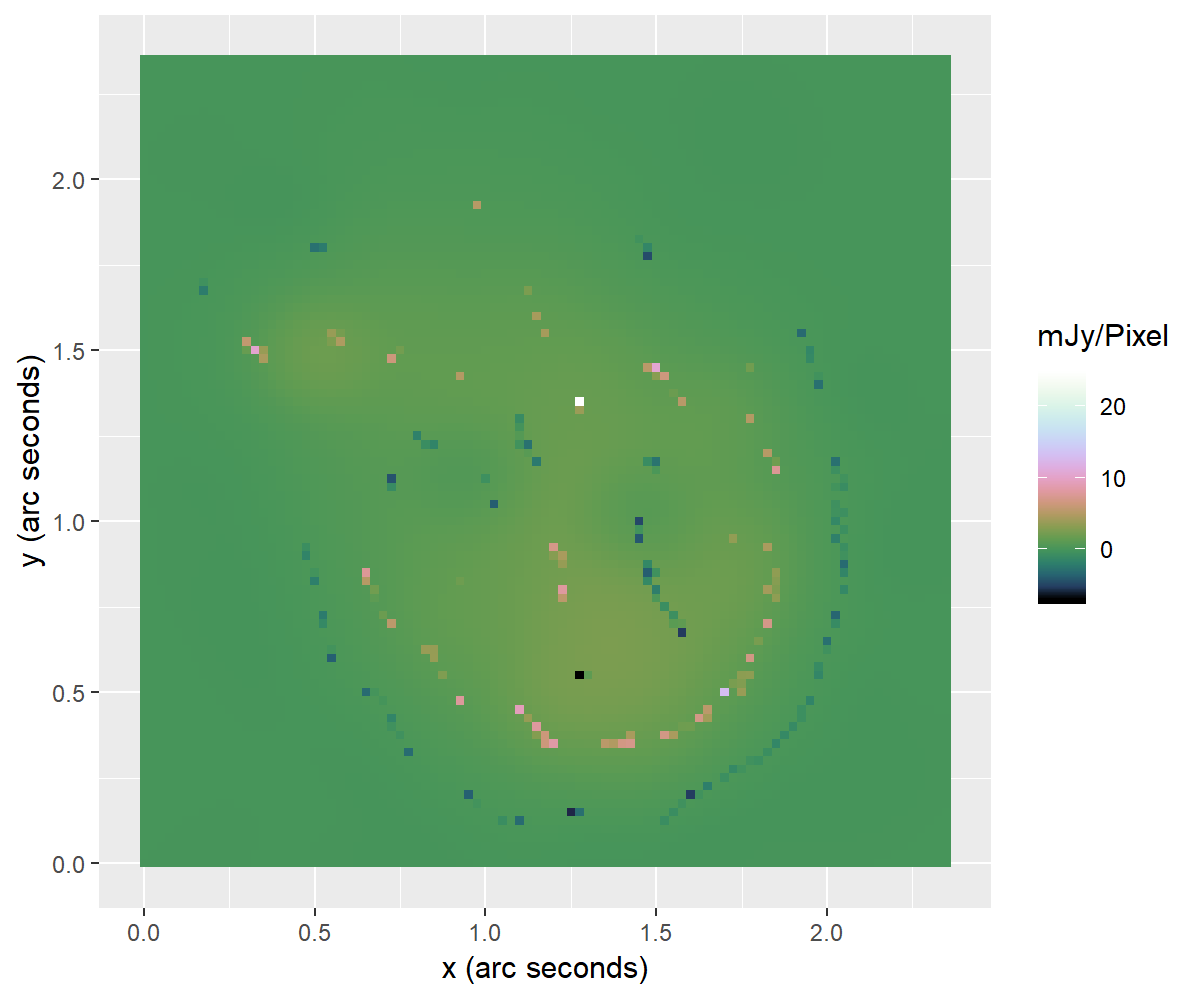
\includegraphics[width=1.00\linewidth]{./chapters/10.results/MSClean/Natural-N132.png}
		\end{subfigure}
		\begin{subfigure}{0.40\linewidth}
			\centering
			\textbf{Restored image}
			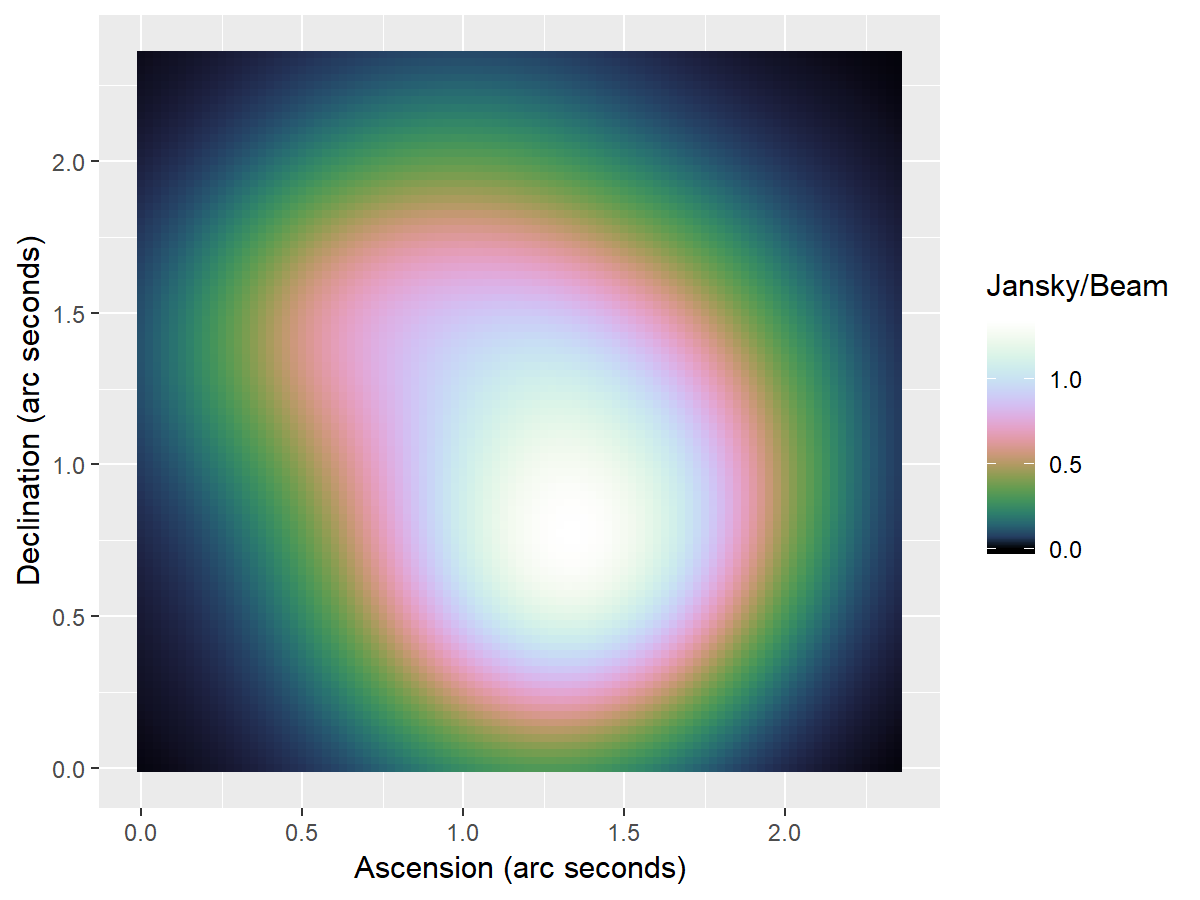
\includegraphics[width=1.00\linewidth]{./chapters/10.results/MSClean/Natural-image-N132.png}
		\end{subfigure}
		\caption{Multi-scale CLEAN.}
	\end{subfigure}
	\begin{subfigure}[b]{1.0\linewidth}
		\centering
		\begin{subfigure}{0.40\linewidth}
			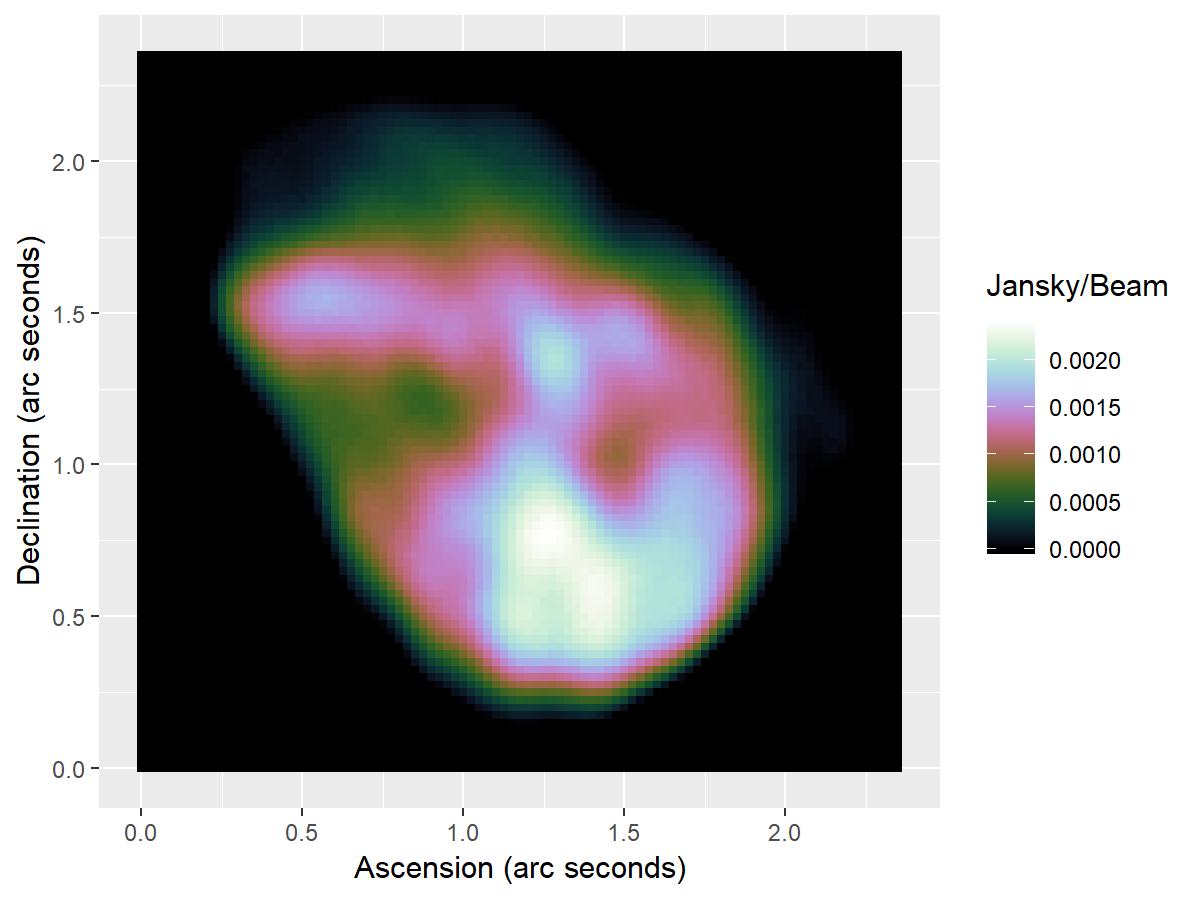
\includegraphics[width=1.00\linewidth]{./chapters/10.results/SerialCD/CD-N132.png}
		\end{subfigure}
		\begin{subfigure}{0.40\linewidth}
			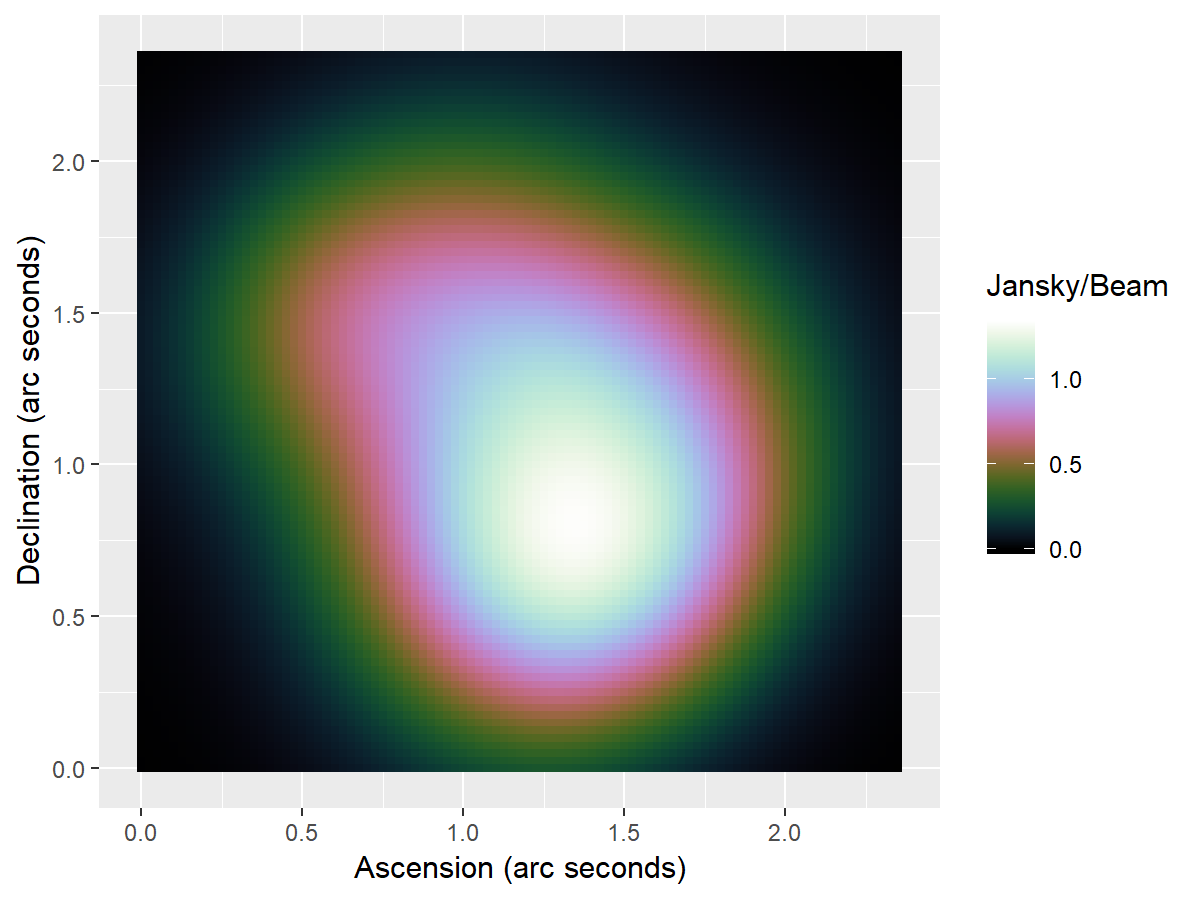
\includegraphics[width=1.00\linewidth]{./chapters/10.results/SerialCD/CD-image-N132.png}
		\end{subfigure}
		
		\caption{Coordinate descent with elastic net.}
	\end{subfigure}
	\begin{subfigure}[b]{1.0\linewidth}
		\centering
		\begin{subfigure}{0.40\linewidth}
			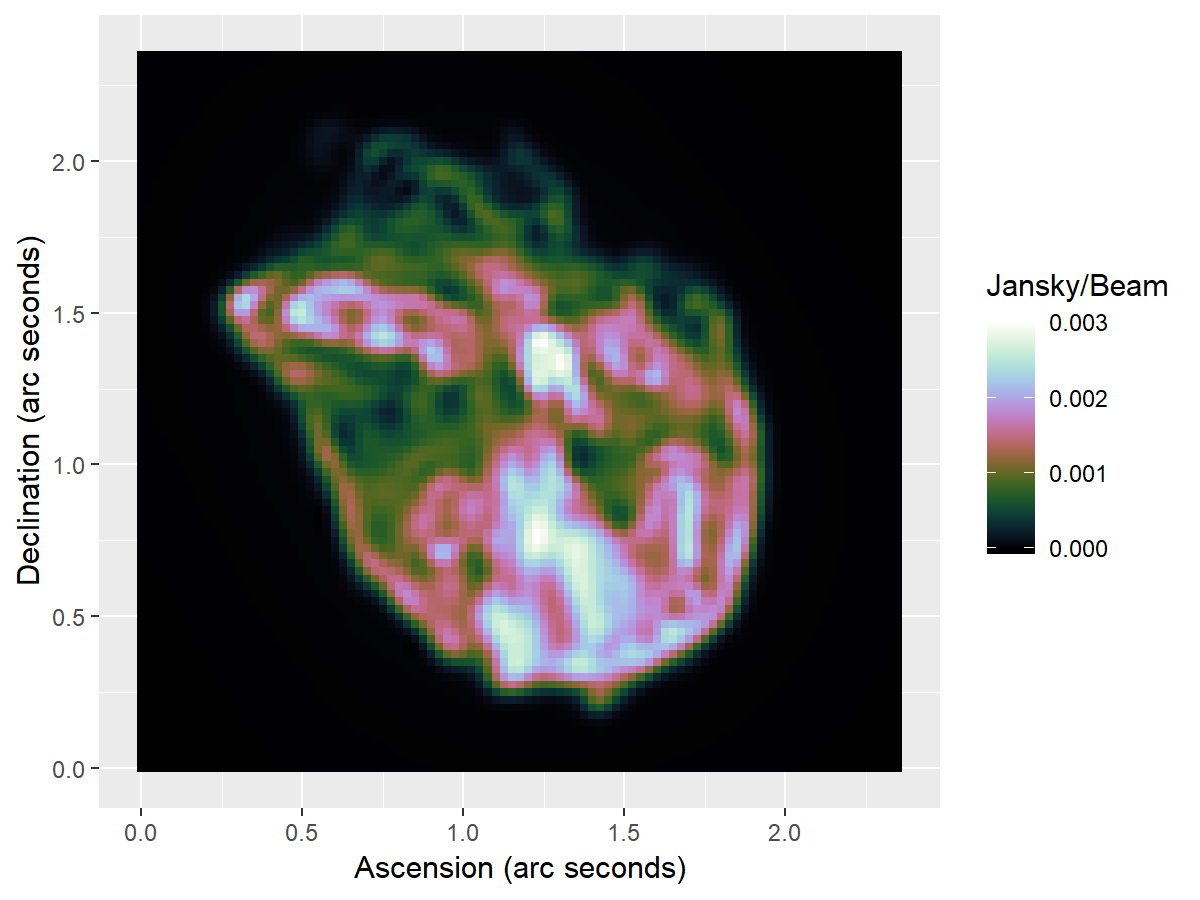
\includegraphics[width=1.00\linewidth]{./chapters/10.results/iuwt/iuwt-N132.png}
		\end{subfigure}
		\begin{subfigure}{0.40\linewidth}
			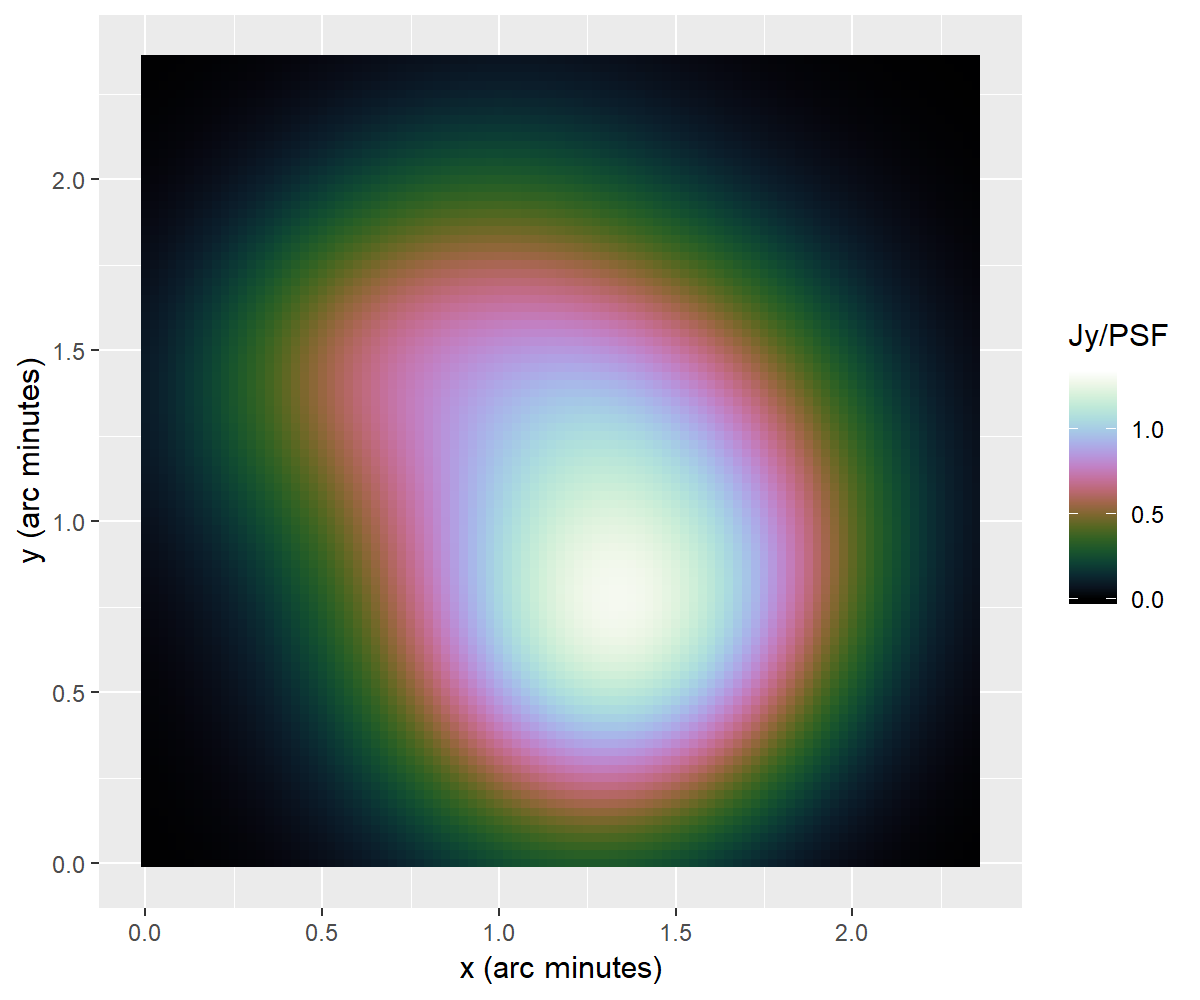
\includegraphics[width=1.00\linewidth]{./chapters/10.results/iuwt/iuwt-image-N132.png}
		\end{subfigure}
		\caption{MORESANE (IUWT).}
	\end{subfigure}

	\caption{Comparison on the N132D supernova-remnant.}
	\label{results:cleancomp::N132:figure}
\end{figure}

In Figure \ref{results:cleancomp::N132:figure} we compare the model- and restored images of the three algorithms. The restored images of the three algorithms overall contain similar structures. The main difference is the resulting magnitude: The restored image of multi-scale CLEAN  has the highest pixel magnitude, while the restored image of MORESANE leads to the lowest pixel magnitude. Remember: MORESANE has left significant emissions in the residual image, while multi-scale CLEAN has removed almost all the relevant emissions. This leads to a difference in the magnitudes of the restored image.

The model images on the other hand have considerable differences. Multi-scale CLEAN chose to reconstruct the supernova-remnant with mostly single pixels, containing both significant positive and negative values. The large negative values forced us to use a different color axis for the model image. With multi-scale deconvolution, CLEAN has a model for extended emissions. But in this case, CLEAN has chosen to explain the emission mainly with single pixels. Multi-scale CLEAN has used negative pixels instead of reducing the magnitude of the pixels already in the model image. It has surrounded the supernova-remnant with negative pixels, and added a few negative pixels inside the remnant.

Coordinate descent with the elastic net regularization has reconstructed a smoother version of the multi-scale CLEAN model image. It does not contain any negative pixel values, and the resulting structure seems plausible. The MORESANE model image contains similar structures, with bright pixels at similar locations. But the MORESANE model image contains more details. Now the question is whether the retrieved structures by coordinate descent and MORESANE are plausible, and may have super-resolved the N132D supernova-remnant.

\newpage

To ensure the structures of the coordinate descent and MORESANE model images are plausible, we compare them to the restored image of briggs-weighted multi-scale CLEAN on the same data. There are three main visibility weighting scheme for the gridder that lead to different $PSF$s from the same measurements: Natural, uniform, and Briggs\cite{briggsWeighting}. Natural weighting scheme leads to an image with a lower noise level, but a wider $PSF$. Uniform weighting leads to a higher noise level, but to a $PSF$ which is more concentrated around a single pixel. Briggs weighting is a scheme combining the best from both worlds, receiving an image with acceptable noise level while getting a more concentrated $PSF$. As such it is widely used in radio astronomy image reconstruction. Our gridder implements the natural weighting scheme only.

We compare the coordinate descent and MORESANE reconstruction with the briggs-weighted multi-scale CLEAN restored image in Figure \ref{results:cleancomp:N132:truth}. Here, we compare if the structures of the MORESANE and coordinate descent model images are plausible, and therefore a super-resolved reconstruction of the N132D supernova-remnant.

\begin{figure}[h]
	\centering
	\begin{subfigure}{0.3\linewidth}
		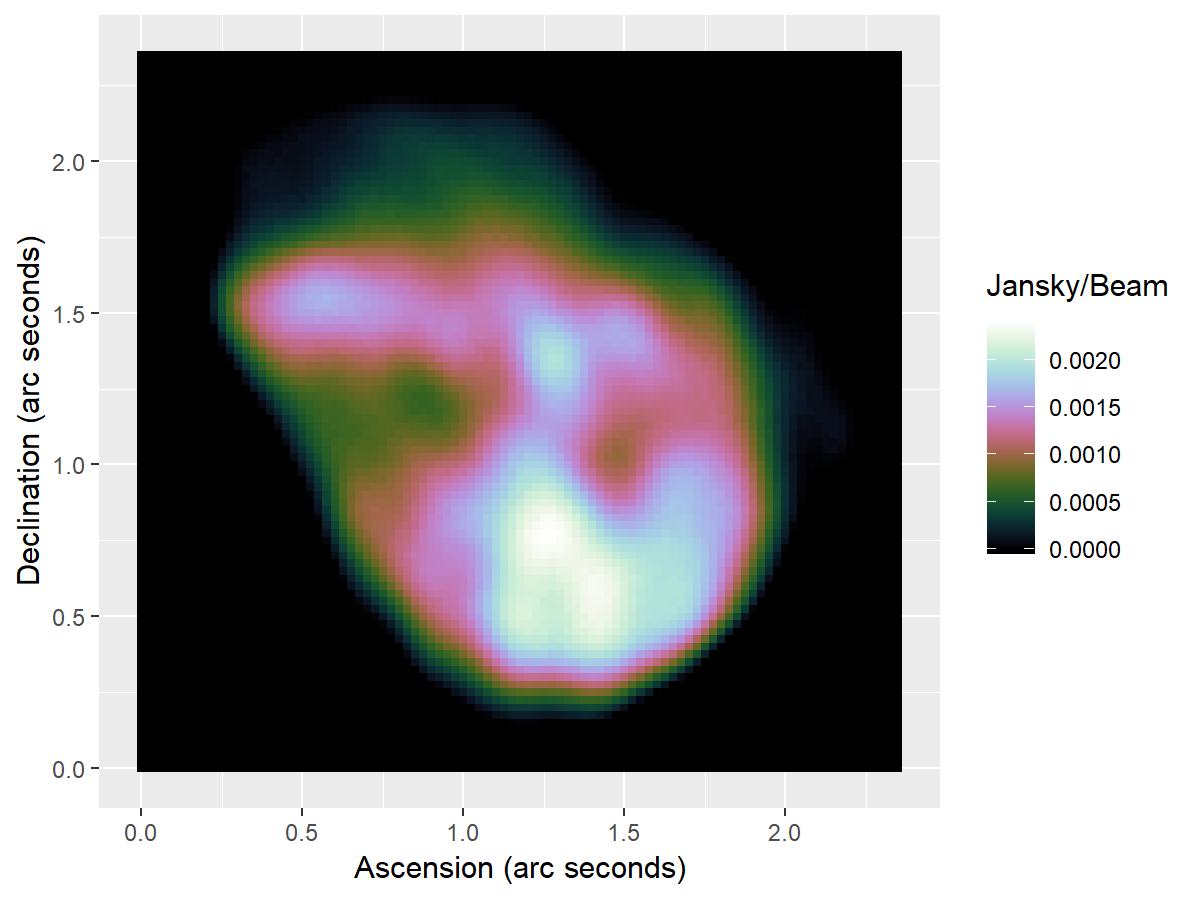
\includegraphics[width=1.00\linewidth]{./chapters/10.results/SerialCD/CD-N132.png}
		\caption{CD}
	\end{subfigure}
	\begin{subfigure}{0.3\linewidth}
		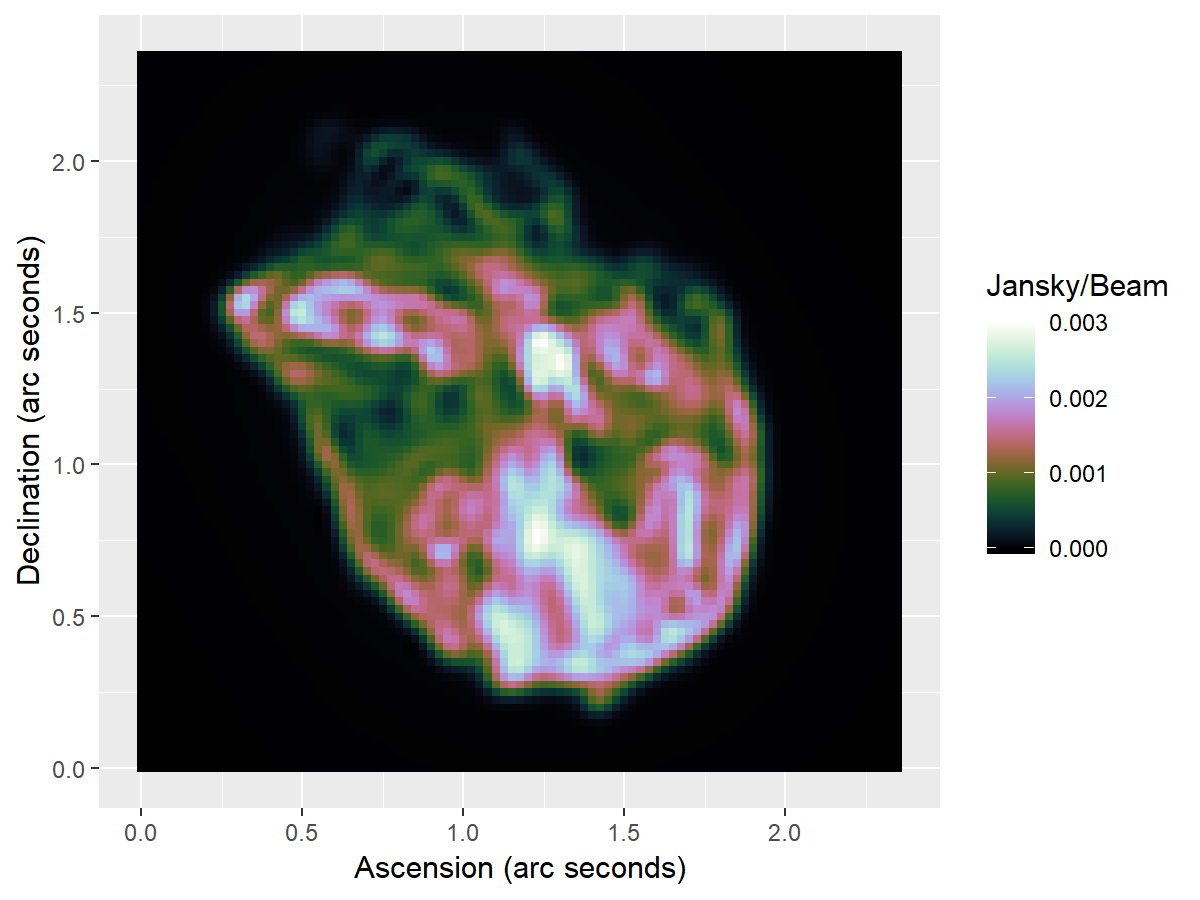
\includegraphics[width=1.00\linewidth]{./chapters/10.results/iuwt/iuwt-N132.png}
		\caption{IUWT}
	\end{subfigure}
	\begin{subfigure}{0.3\linewidth}
		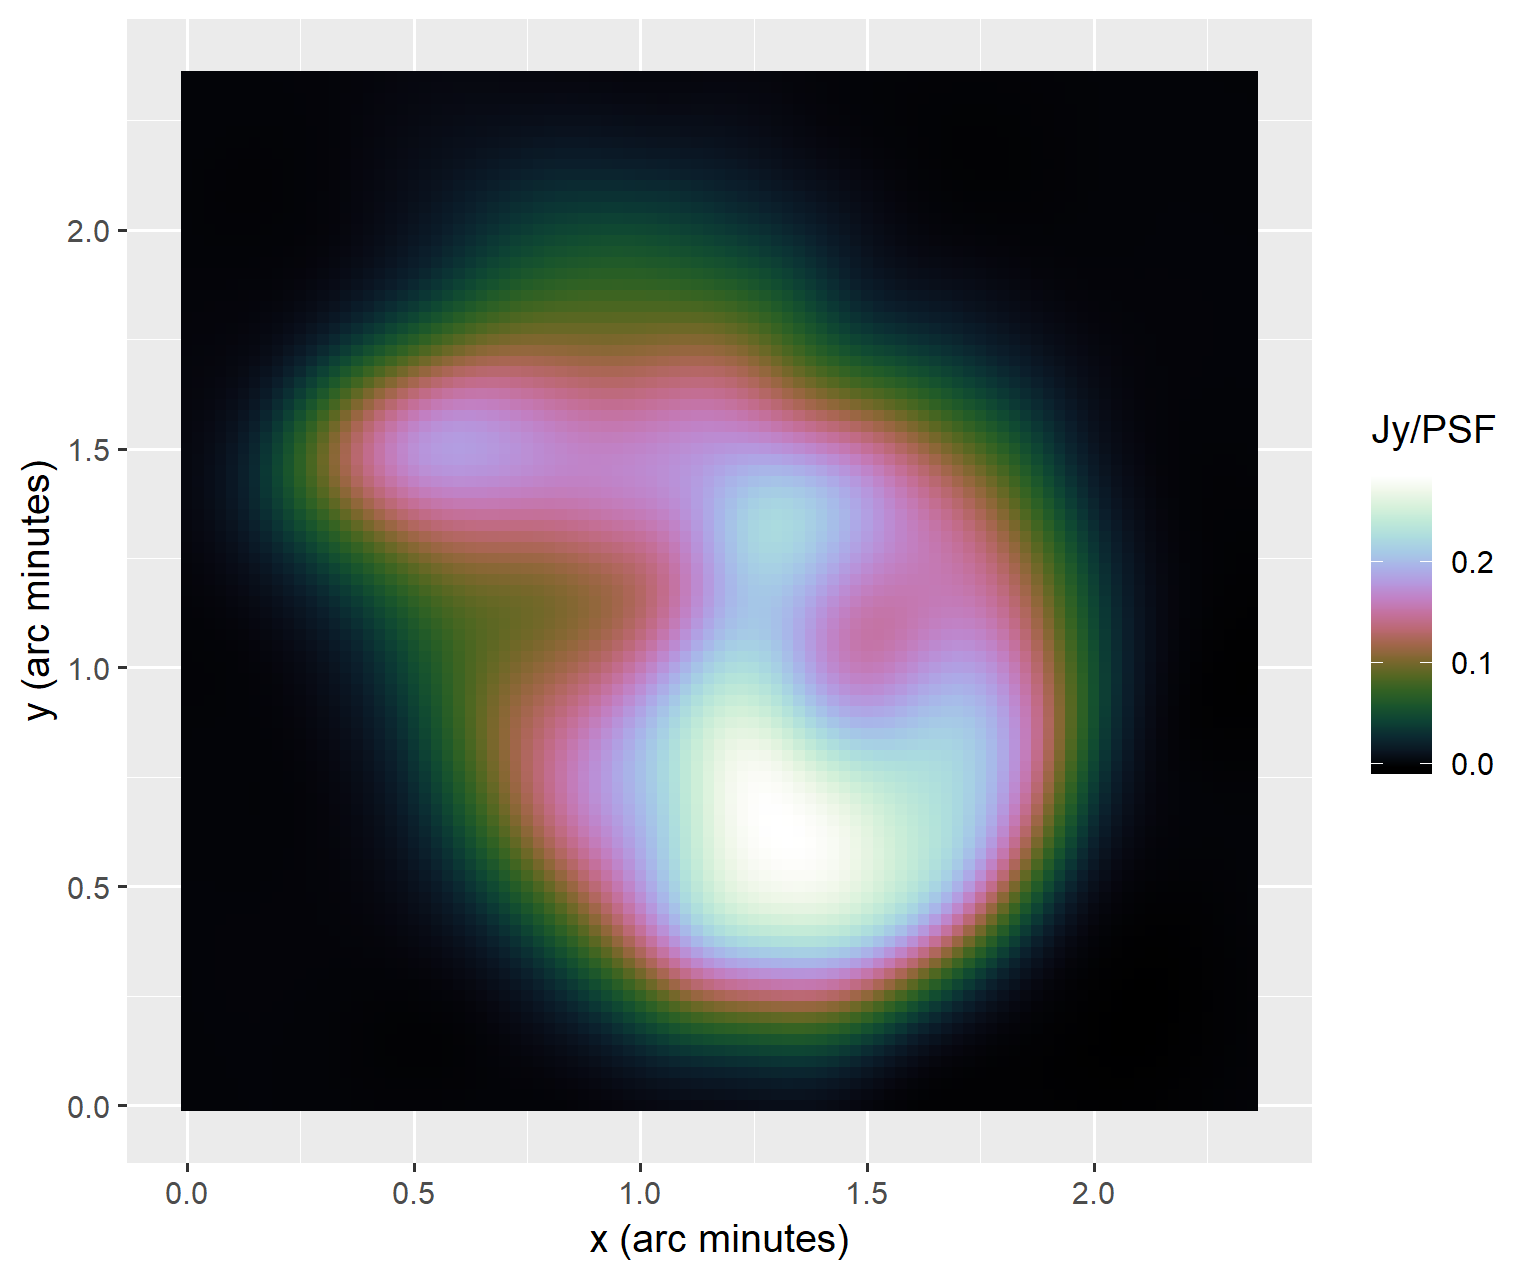
\includegraphics[width=1.00\linewidth]{./chapters/10.results/MSClean/Briggs-N132.png}
		\caption{Briggs MS-CLEAN}
	\end{subfigure}
	\caption{Comparison with briggs-weighted multi-scale CLEAN as Ground Truth.}
	\label{results:cleancomp:N132:truth}
\end{figure}

The model image of the coordinate descent reconstruction closely resembles the structures in the briggs-weighted multi-scale CLEAN restored image. Coordinate descent reconstructed a bright core and a distinct 'horizontal' arm, similar to briggs-weighted CLEAN. The MORESANE (IUWT) model image contains roughly similar structures, but adds more details. In this work, we cannot verify the more detailed structures of the MORESANE model image of the N132D supernova-remnant.

\subsubsection{Influence of calibration errors}

\begin{figure}[!ht]
	\centering
	\begin{subfigure}[b]{0.82\linewidth}
		\centering
		\begin{subfigure}{0.45\linewidth}
			\centering
			\textbf{Model image}
			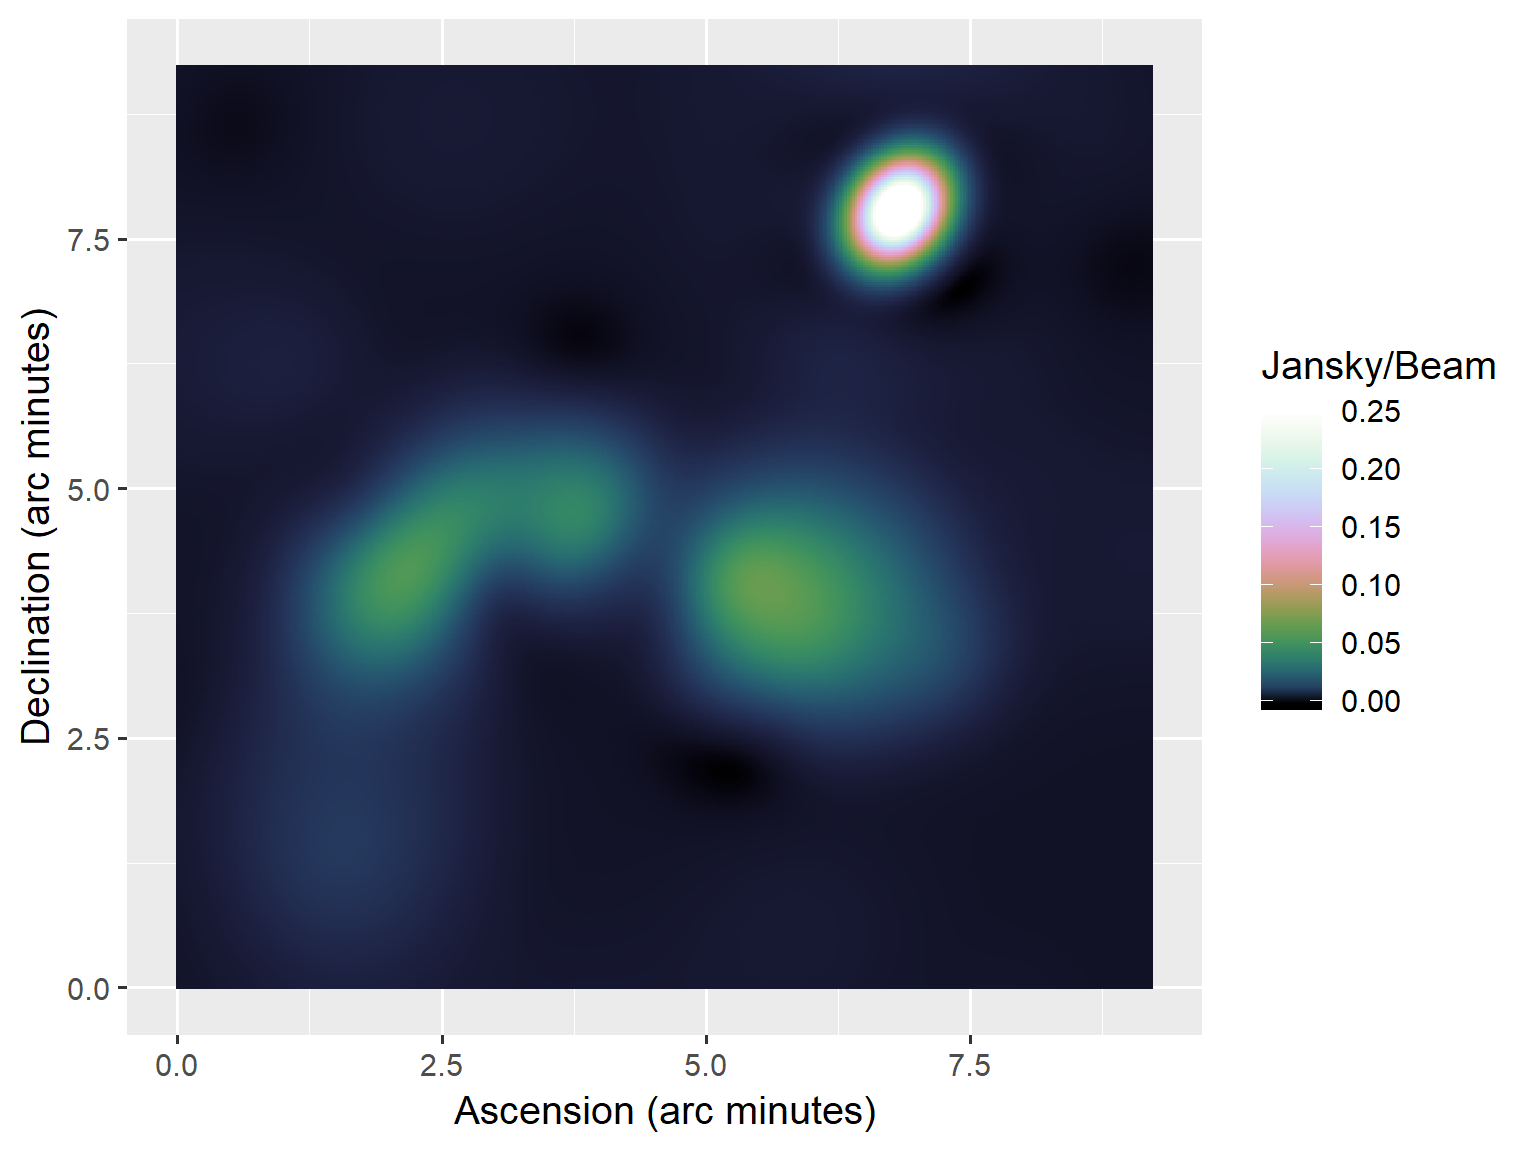
\includegraphics[width=1.00\linewidth]{./chapters/10.results/MSClean/Natural-Calibration.png}
		\end{subfigure}
		\begin{subfigure}{0.45\linewidth}
			\centering
			\textbf{Restored image}
			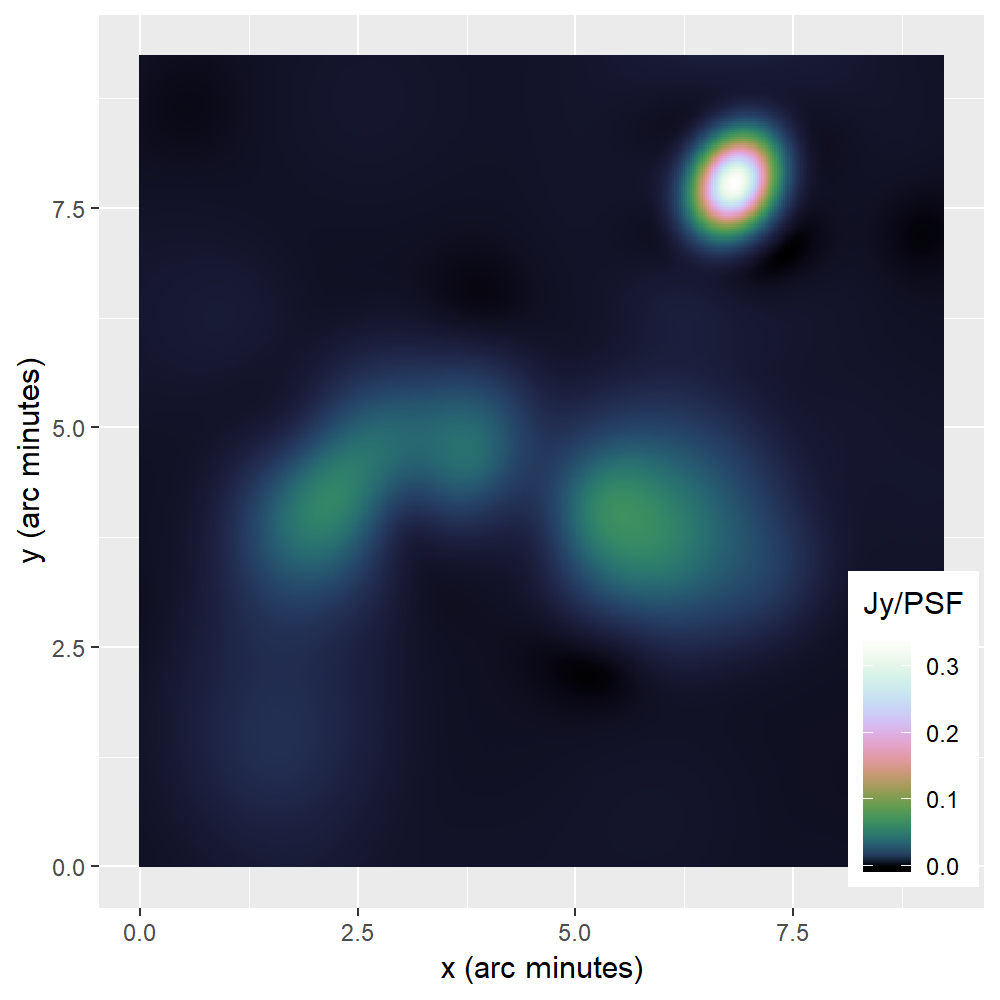
\includegraphics[width=1.00\linewidth]{./chapters/10.results/MSClean/Natural-image-Calibration.png}
		\end{subfigure}
		\caption{Multi-scale CLEAN}
	\end{subfigure}
	\begin{subfigure}[b]{0.82\linewidth}
		\centering
		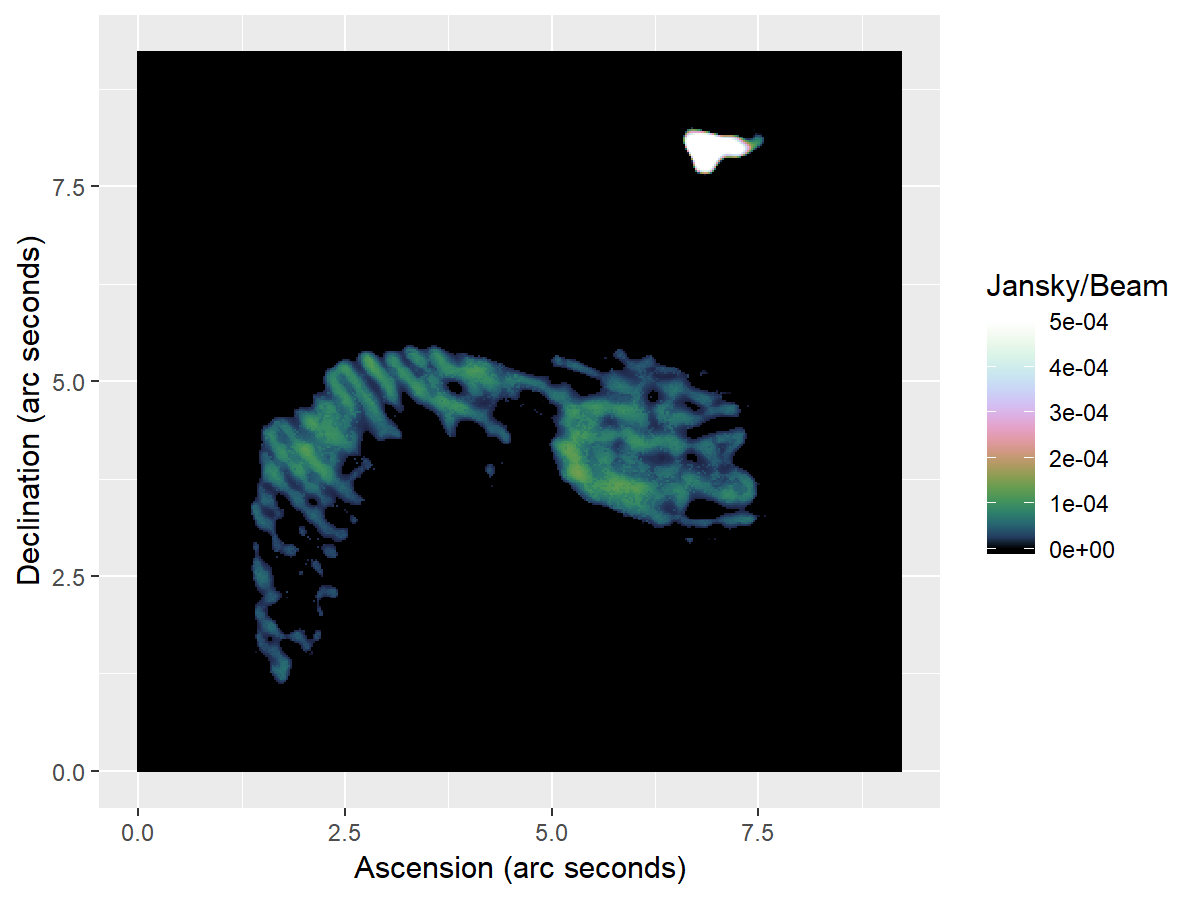
\includegraphics[width=0.45\linewidth]{./chapters/10.results/SerialCD/CD-Calibration.png}
		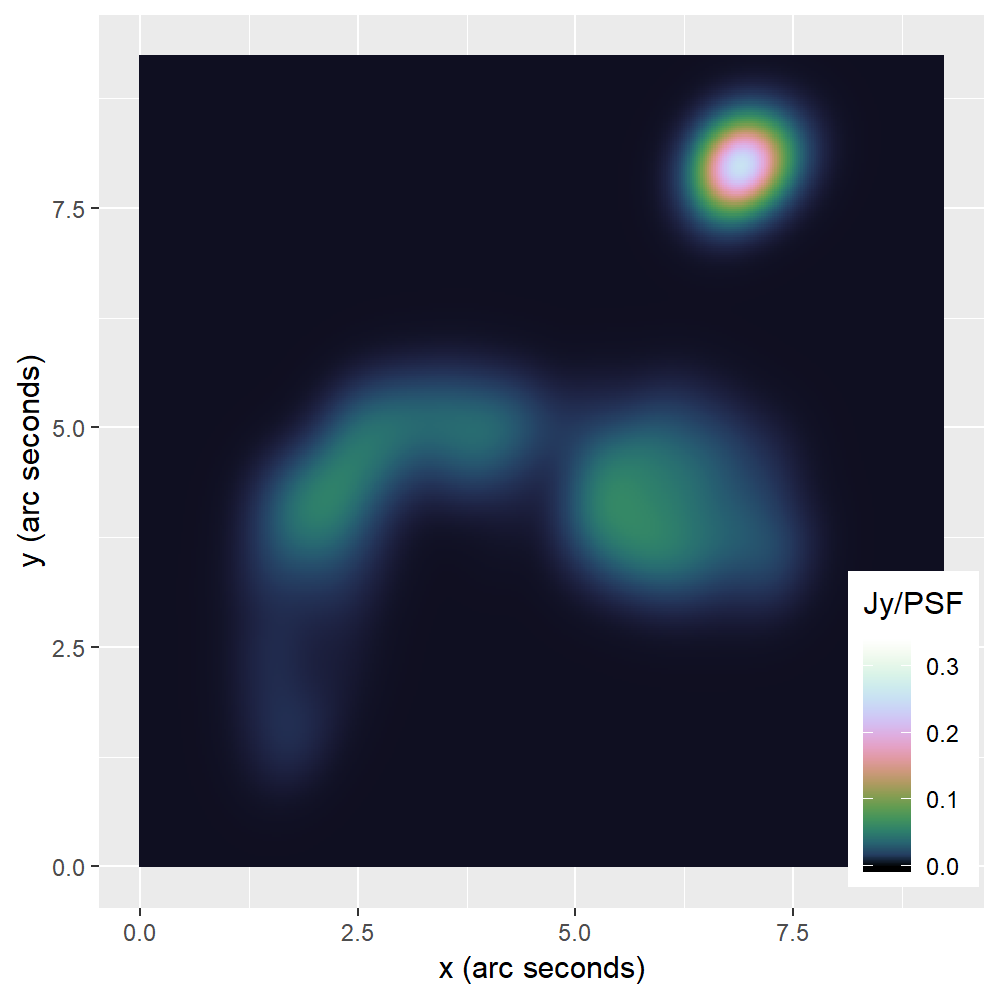
\includegraphics[width=0.45\linewidth]{./chapters/10.results/SerialCD/CD-image-Calibration.png}
		\caption{Coordinate Descent with elastic net.}
	\end{subfigure}
	\begin{subfigure}[b]{0.82\linewidth}
		\centering
		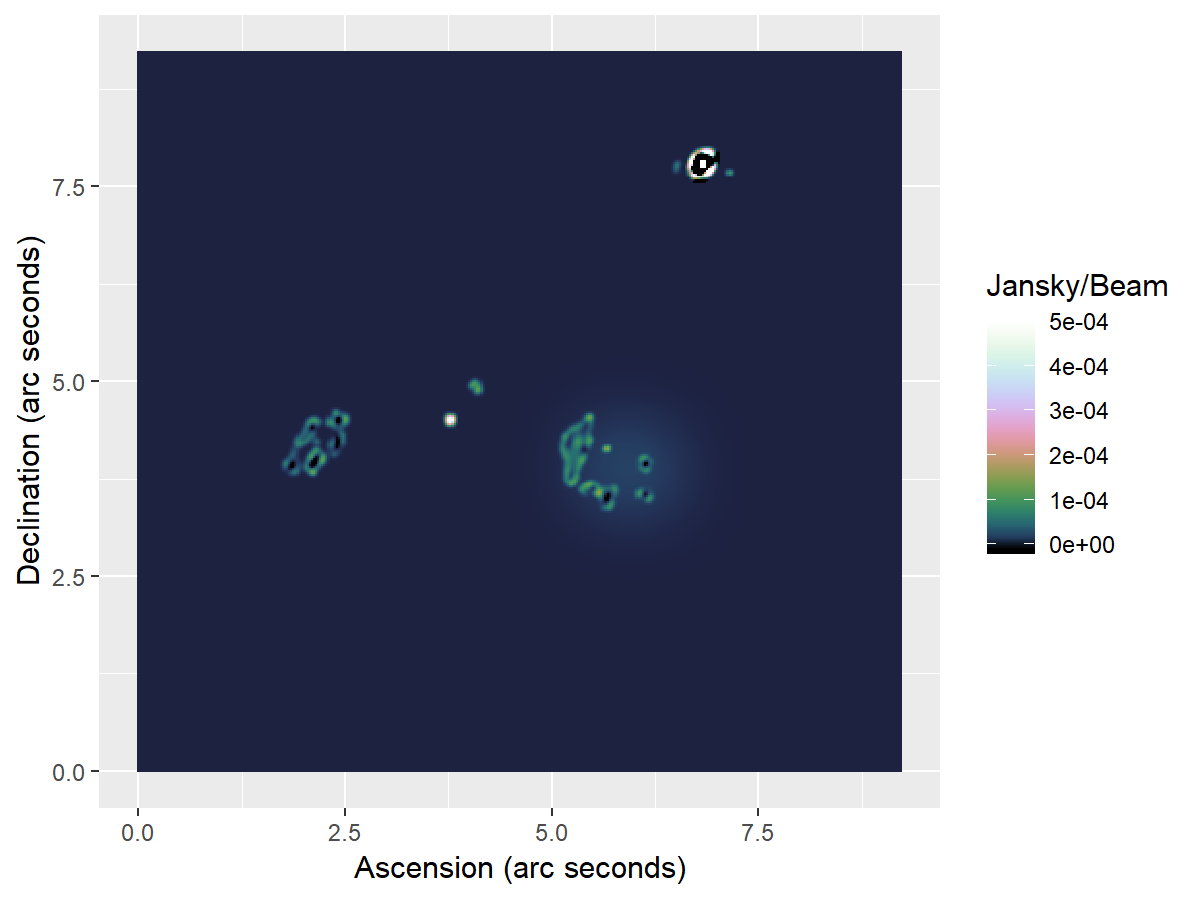
\includegraphics[width=0.45\linewidth]{./chapters/10.results/iuwt/iuwt-Calibration.png}
		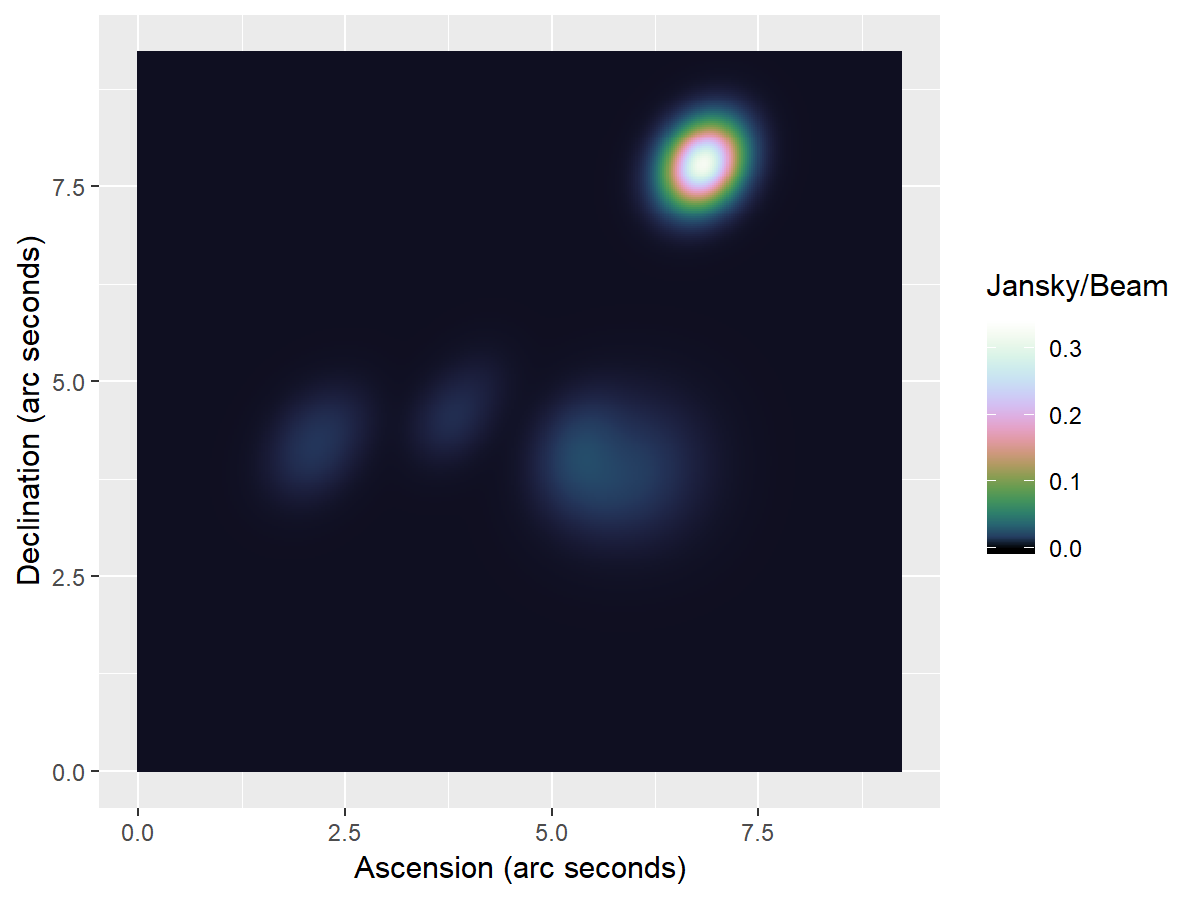
\includegraphics[width=0.45\linewidth]{./chapters/10.results/iuwt/iuwt-image-Calibration.png}
		\caption{MORESANE (IUWT)}
	\end{subfigure}
	\caption{Influence of calibration errors}
	\label{results:cleancomp::calib:figure}
\end{figure}

In this section, we compare the model and restored images of an area influenced by calibration errors. The image section is located on the center-right of the full image. We see two faint extended emissions, next to a point source with calibration errors. The phase calibration in this area of the image is imperfect, which leads to a de-correlation artifacts (wave-like artifacts around the point source). The de-correlation artifacts are mainly visible in the residual images. But they also influence the model- and restored images. Figure \ref{results:cleancomp::calib:figure} compares the model and restored images of the three algorithms.

The multi-scale CLEAN and MORESANE model images contain significant negative pixel values in this section of the reconstruction. For a reasonable comparison, we had to clip the negative values, which are now shown as black pixels in the model images. Due to the bright point source in the image, we also clipped the maximum positive value for all model images.

The model image of Multi-scale CLEAN contains a straight-forward representation of the two extended emissions. Significant negative pixels are placed around the extended emissions. The point source contains several 'rings' of negative and positive pixels, related to the calibration errors. The serial coordinate descent algorithm is forbidden to use negative pixels. The calibration errors result in a 'smearing' of the point source in the horizontal directions. The two extended emissions also get influenced by the calibration errors with coordinate descent. MORESANE on the other hand misses large parts of the left-hand-side extended emission. The point source in the image is reconstructed similar to multi-scale CLEAN, containing rings of significant negative pixels.

These differences in the model images also result in variations of the restored image. The multi-scale CLEAN restored image contains several areas of negative emission. The coordinate descent restored image does not contain any negative pixels. The two extended emissions are also similar in shape and pixel value to multi-scale CLEAN. The restored image of MORESANE is missing parts of the extended emission.

\newpage

\begin{figure}[h]
	\centering
	\begin{subfigure}[b]{0.3\linewidth}
		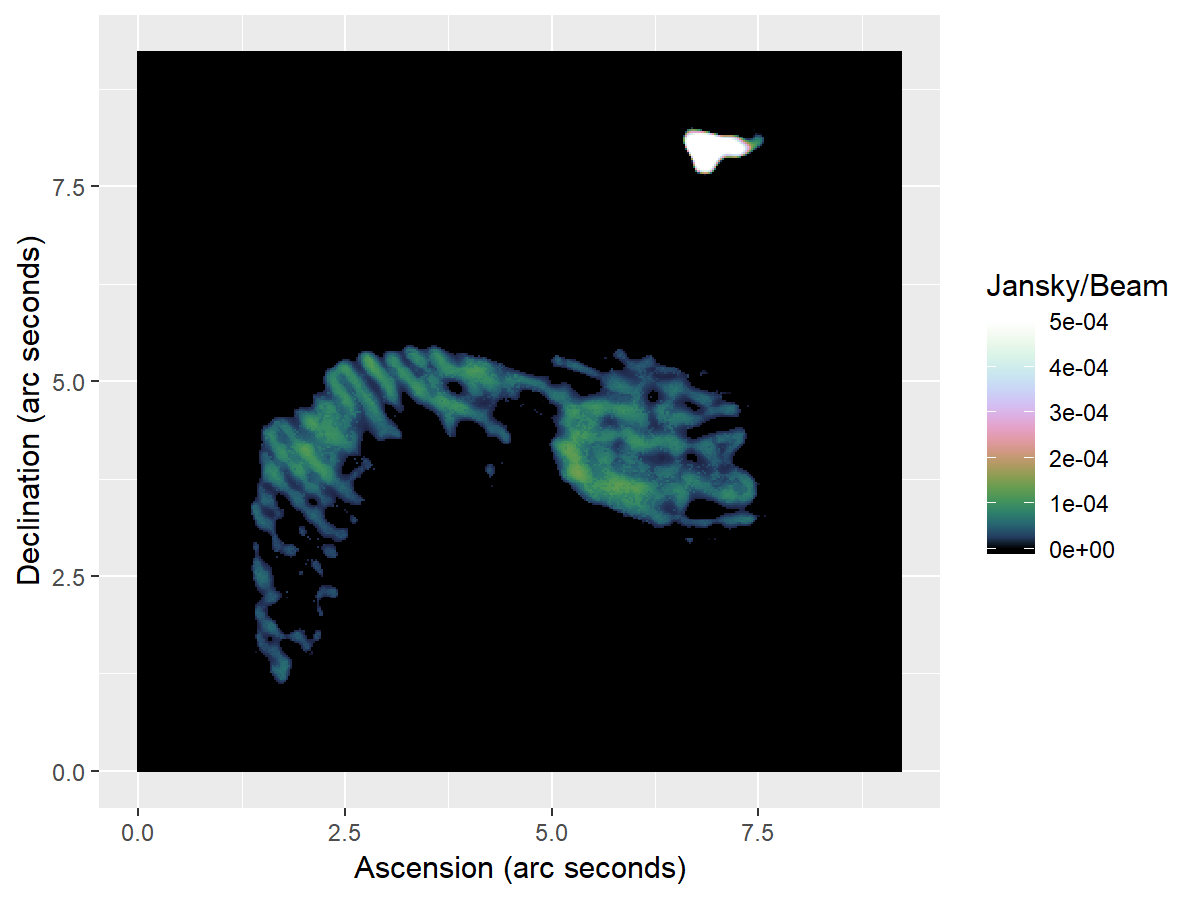
\includegraphics[width=1.00\linewidth]{./chapters/10.results/SerialCD/CD-Calibration.png}
		\caption{Coordinate Descent}
	\end{subfigure}
	\begin{subfigure}[b]{0.3\linewidth}
		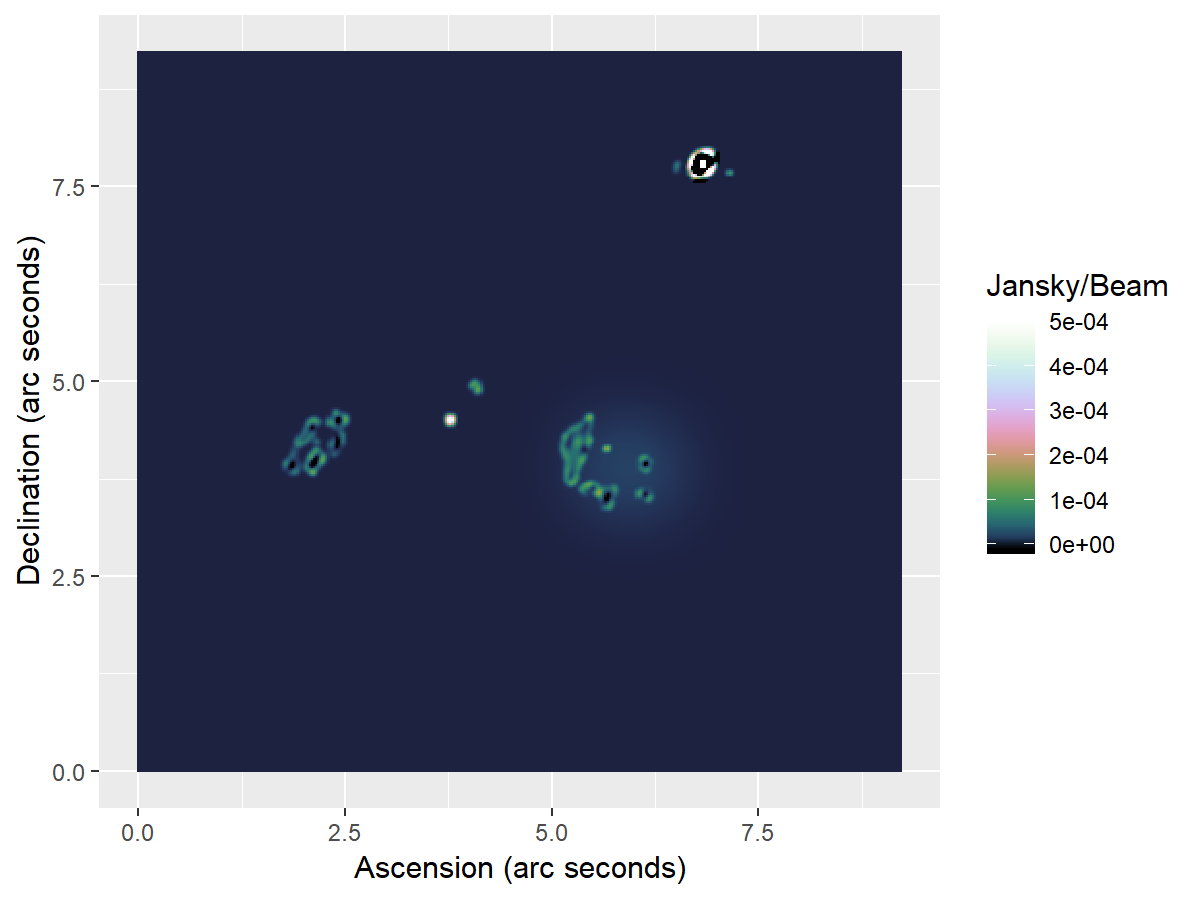
\includegraphics[width=1.00\linewidth]{./chapters/10.results/iuwt/iuwt-Calibration.png}
		\caption{IUWT}
	\end{subfigure}
	\begin{subfigure}[b]{0.3\linewidth}
		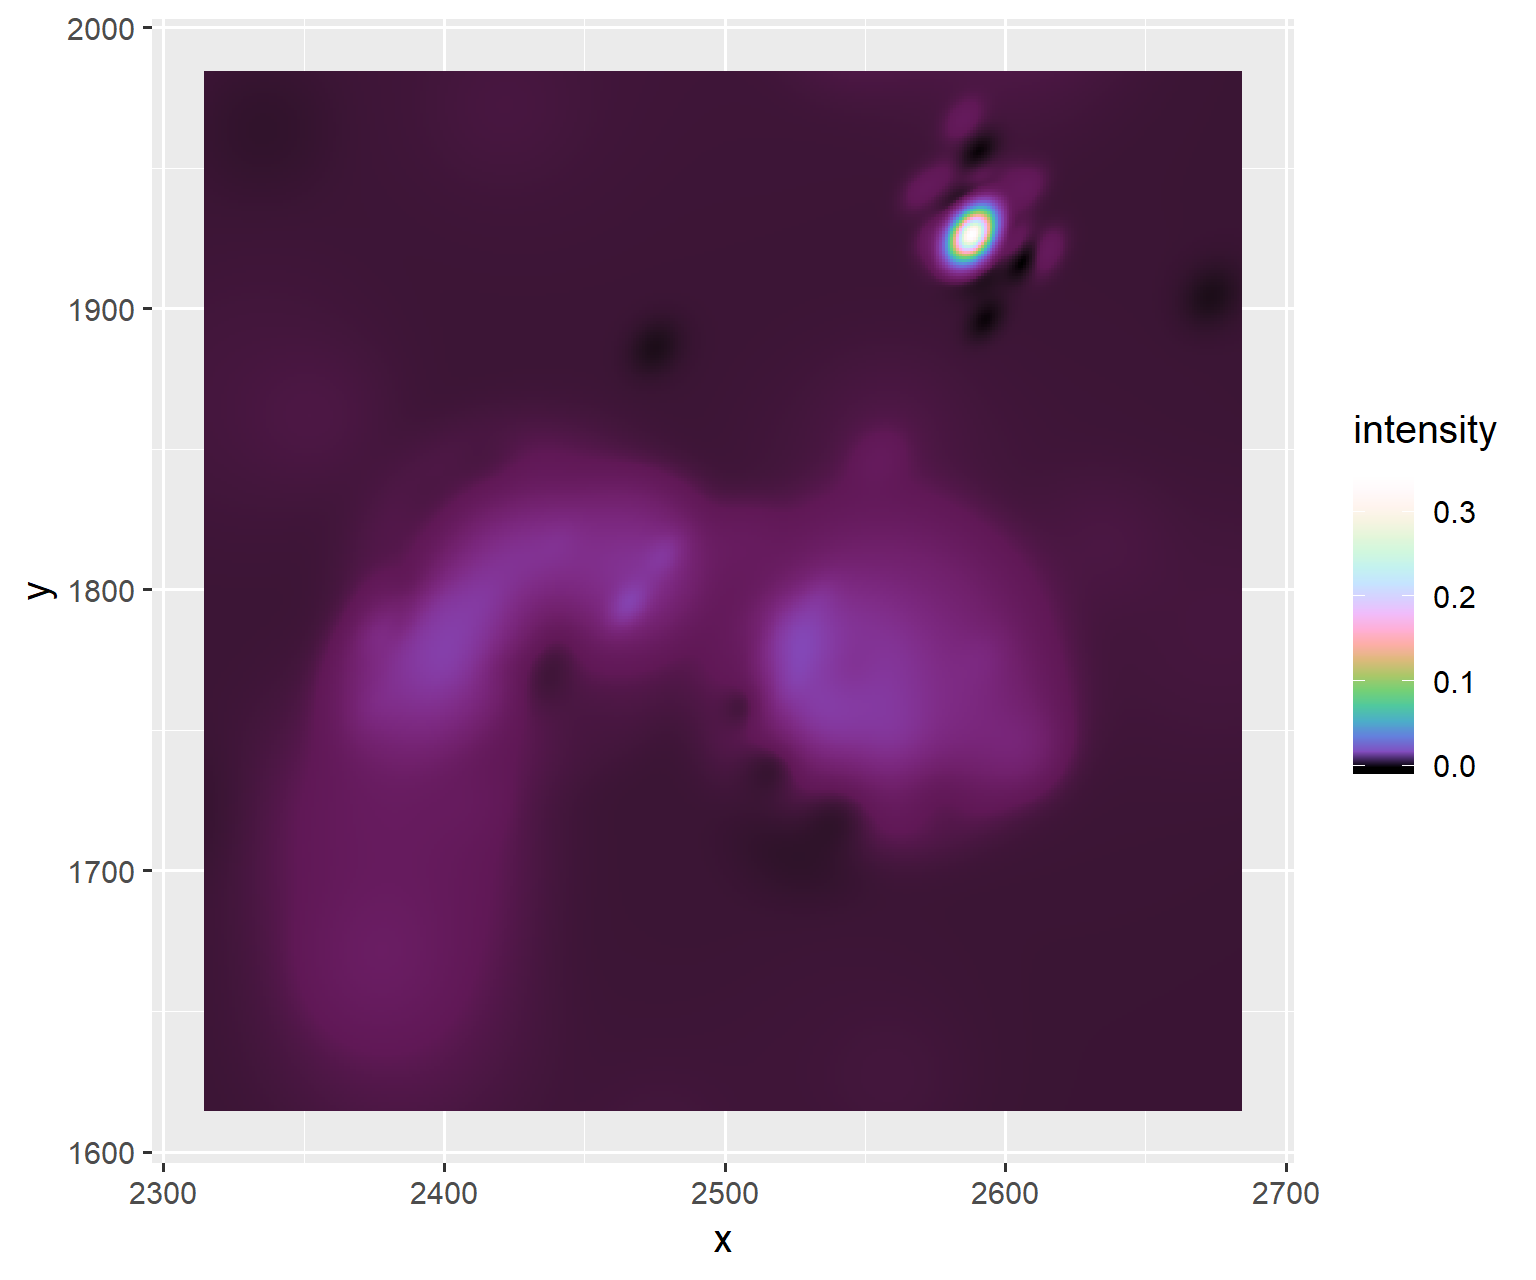
\includegraphics[width=1.00\linewidth]{./chapters/10.results/MSClean/Briggs-Calibration.png}
		\caption{Briggs CLEAN}
	\end{subfigure}

	\caption{Comparison to briggs-weighted multi-scale CLEAN as Ground Truth.}
	\label{results:cleancomp::calib:figure}
\end{figure}

Lastly, we again compare the model images of coordinate descent and MORESANE (IUWT) with the restored image of briggs-weighted multi-scale CLEAN. The briggs-weighted restored image has reconstructed more details in the two extended emissions. The left-hand-side emission contains two point sources at its border, while the right-hand-side emission contains a crescent. The model image of the coordinate descent algorithm has detected structures of the crescent, but has missed the two point sources. MORESANE did detected the point sources and the crescent in the extended emission, but did miss large parts of the actual emission.

Overall, serial coordinate descent with elastic net regularization has produced a restored image with similar structures to multi-scale CLEAN on the same observation. Coordinate descent has left a residual image with a higher pixel magnitudes than CLEAN. This can be improved by adding a similar auto-masking strategy to serial coordinate descent. The model images resulting from the elastic net regularization is more plausible than multi-scale CLEAN on this observation. It has produced a plausible super-resolution of the N132D supernova-remnant, and has found other plausible structures in extended emissions. However, its model image also seems to be more susceptible to calibration errors. 

The MORESANE algorithm was reported to generally produce higher-quality reconstructions than multi-scale CLEAN, while also needing more computing resources \cite{dabbech2015moresane, offringa2017optimized}. In our test, multi-scale CLEAN has produced a higher quality reconstruction. MORESANE has various tuning parameters which influence the reconstruction quality. It is possible that we used sub-optimal parameters for the reconstruction. We modified several parameters of the MORESANE algorithm, but could not improve the results reported here.

The WSCLEAN software package has an option for multi-scale CLEAN, which forces the model image to be non-negative. However, we have not compared those results to the serial coordinate descent reconstruction. This option has lead multi-scale CLEAN to an overall worse reconstruction, with higher pixel magnitudes in the residual image, and longer wall-clock time. With our tuning parameter setting, it required more than twice the number of Major cycles than previous (14 Major cycles compared to 6).

The serial coordinate descent algorithm needed more computing resources than multi-scale CLEAN. The main difference is in the number of Minor cycles: Multi-scale CLEAN needed overall 15'000 iterations, while serial coordinate descent needed 100'000 iterations. The number of Major cycles was similar for both algorithms: Multi-scale CLEAN converged within 6 Major cycles, and serial coordinate descent within 5. Note that the number of Major cycles of the two algorithms is only roughly comparable. In this project, we use a different gridder than WSCLEAN, and we have not ensured our stopping criterion is identical to WSCLEAN. 

We now test how we can speed-up first serial coordinate descent, and then parallel coordinate descent to beat multi-scale CLEAN in terms of reconstruction time.

%Figure \ref{results:cleancomp:figure} shows the reconstruction of both briggs-weighted multi-scale CLEAN and the naturally weighted coordinate descent reconstruction. We used a regularization parameter of $\lambda = 1.0 * Lipschitz$ and $\alpha = 0.01$. The elastic net regularization is biased heavily towards the L2 norm. We stopped the serial coordinate descent if every possible pixel change is below $\epsilon = 1e^{-5}$. We use these parameters for the whole project unless we specify otherwise.

%Multi-scale reconstructed its image within 6 Major and 14 thousand Minor cycle iterations. Our serial coordinate descent algorithm converged after 5 Major cycles and used 100 thousand iterations to converge. Our algorithm required roughly 8 times more iterations. It took a total of 35 minutes to reconstruct an image on an Intel Xeon E3-1505M with 8 logical cores. On this data set, our algorithm used one Major cycle less than multi-scale CLEAN. However, the number of Major cycles is not directly comparable. We do not use the identical criteria to initiate another Major cycle: At the beginning of each deconvolution, we check the maximum pixel difference. If it is below $\epsilon_{major} = 1e^{-4}$, we stop the reconstruction. We have not compared our stopping criterion to WSCLEAN. As such, the number of Major cycles are only a rough comparison. Our serial coordinate descent uses a similar number of Major cycles as multi-scale CLEAN.



\subsection{$PSF$ approximation with serial coordinate descent} \label{results:gradients}
In this section, we test our main hypothesis on the MeerKAT LMC data: The Major cycle allows us to use an approximation of the true $PSF$ in Minor cycle. We believe this can be exploited. We may be able to use a fraction of the true $PSF$ in the serial coordinate descent algorithm, potentially speeding up the deconvolution and simplifying distribution.

An example of the $PSF$ approximation is shown Figure \ref{results:gradients:clark}. Instead of the full $PSF$, we use a window around the center of the $PSF$. The sides of the window are a fraction of the full $PSF$.
\begin{figure}[h]
	\centering
	\begin{subfigure}[b]{0.245\linewidth}
		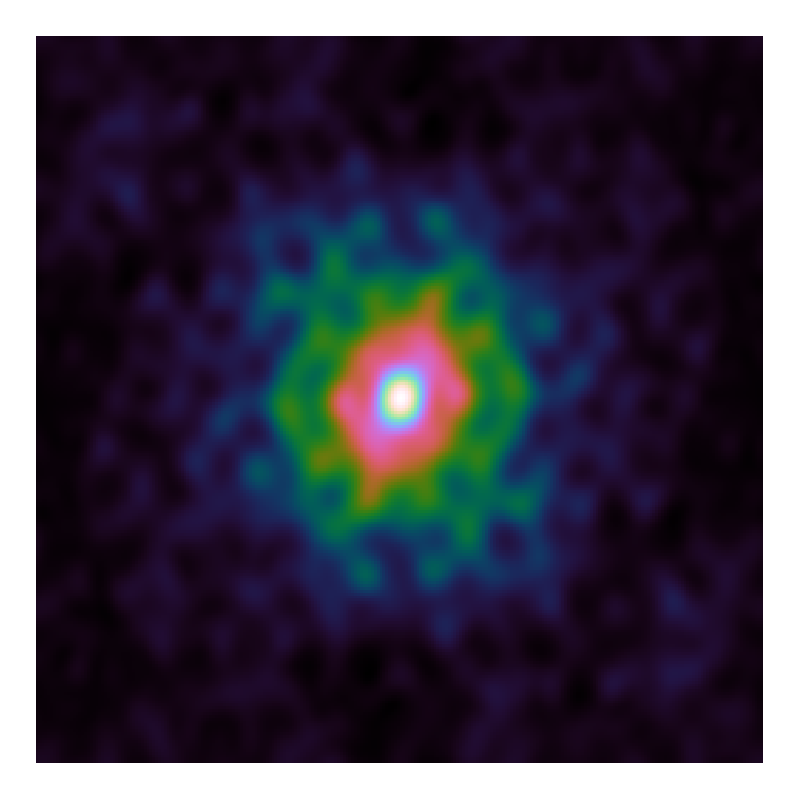
\includegraphics[width=\linewidth, clip, trim= 0.25in 0.25in 0.25in 0.25in]{./chapters/03.cd/simulated/psf.png}
		\caption{Full $PSF$}
	\end{subfigure}
	\begin{subfigure}[b]{0.245\linewidth}
		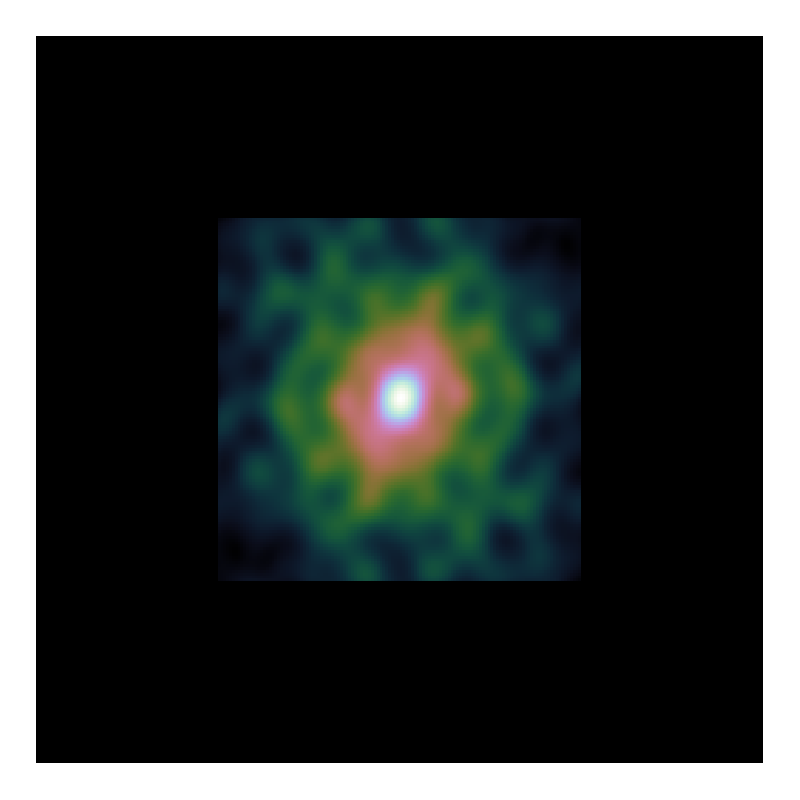
\includegraphics[width=\linewidth, clip, trim= 0.25in 0.25in 0.25in 0.25in]{./chapters/03.cd/simulated/psfCut.png}
		\caption{$\frac{1}{2}PSF$ approximation}
	\end{subfigure}
	\caption{Example of a $PSF$ approximation.}
	\label{results:gradients:clark}
\end{figure}

In this section, we test ever smaller window sizes and observe the convergence speed of our serial coordinate descent algorithm. We developed two methods to exploit an approximate $PSF$ in our serial coordinate descent algorithm: Method 1 'approximate update', and method 2 'approximate deconvolution'. At the start of each Major cycle, we calculate the objective value of the current solution, and track its development for each Major cycle. Finally, we combine the two approximation methods and compare how much we can speed up our serial coordinate descent method.


\subsubsection{Method 1: Approximate update}
As described in Section \ref{gradients:methods:update}, we normally use the product of $PSF \star PSF$ to update the gradient map in each iteration of serial coordinate descent. This method uses the approximate $PSF$ to update the gradient map: $Cut(PSF) \star Cut(PSF)$. With each iteration, the gradient map becomes less accurate. This approximation method is guaranteed to converge to the same result, if we have unlimited number of major cycles.
	
To test the convergence behaviour, we calculate the objective value of the current solution at the start of each Major cycle. We compare the objective value and the wall-clock time of the original serial coordinate descent and the serial coordinate descent using an approximate gradient update. This is a minimization problem, meaning the lowest objective is the most accurate reconstruction (according to the elastic net regularization).

\begin{figure}[h]
	\centering
	\begin{subfigure}[b]{0.58\linewidth}
		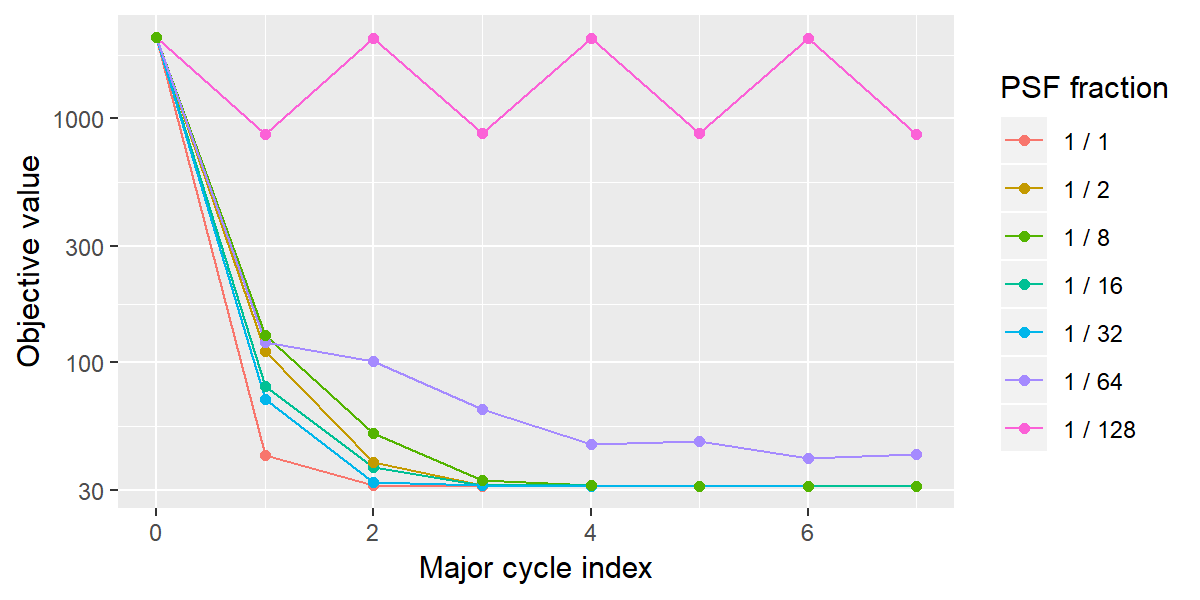
\includegraphics[width=\linewidth]{./chapters/10.results/gradient/ApproxUpdate/size.png}
	\end{subfigure}
	\begin{subfigure}[b]{0.195\linewidth}
		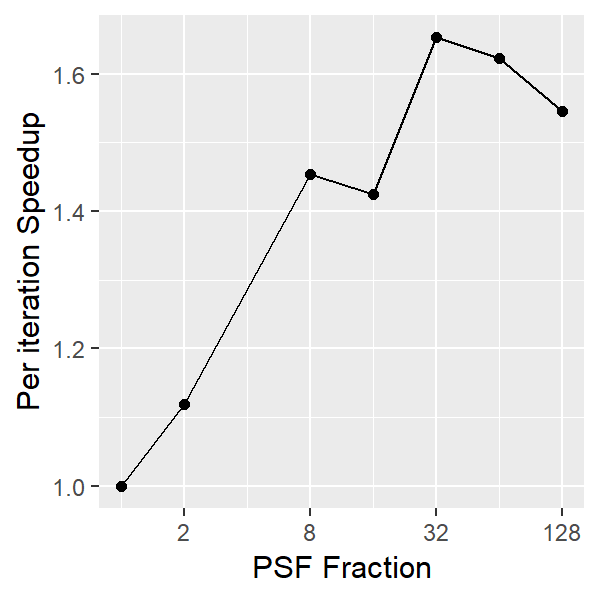
\includegraphics[width=\linewidth]{./chapters/10.results/gradient/ApproxUpdate/speedup_iter.png}
	\end{subfigure}
	\begin{subfigure}[b]{0.195\linewidth}
		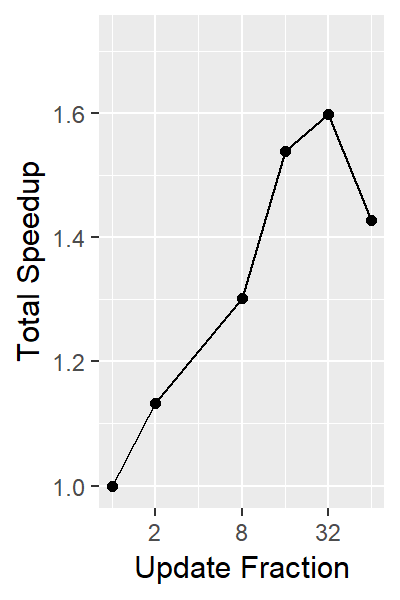
\includegraphics[width=\linewidth]{./chapters/10.results/gradient/ApproxUpdate/speedup_total.png}
	\end{subfigure}
	
	\caption{Convergence of the approximate update method.}
	\label{results:gradients:update}
\end{figure}

Figure \ref{results:gradients:update} shows the convergence rate of the serial coordinate descent algorithm with the approximate update method. Each line represents a run with a specific $PSF$ window. The size of the window are a fraction of the full $PSF$. For example, the full $PSF$ in this test has $3072^2$ pixels. The approximation $\frac{1}{64}$ window is the smallest window around the center of the $PSF$, which is $48^2$ pixels in size. The $\frac{1}{64}$ window is the most aggressive approximation for which the serial coordinate descent algorithm still converges.

We compare two different wall-clock times: The average time necessary for a single serial coordinate descent iteration, and the total time spent in the algorithm. We see from the two speedup curves in Figure \ref{results:gradients:update} that the speedup per iteration increases less than linear with the $PSF$ fraction used in the approximation. Although each iteration becomes cheaper with a smaller $PSF$ window, we may need more iterations to converge to the same result. This is indeed the case for a $PSF$ window smaller than $\frac{1}{32}$. We see a significant drop of the total speedup. Overall with gradient update approximations the serial coordinate descent algorithm can be sped up by a factor of 1.6, if we use $\frac{1}{32}$ window of the full $PSF$.


\subsubsection{Method 2: Approximate deconvolution}
As described in Section \ref{gradients:methods:deconv}, this approximation method uses the same approximation to update the gradient map($Cut(PSF) \star Cut(PSF)$). This approximation method also uses the approximate $PSF$ to initialize the gradient map: $gradients = residuals \star Cut(PSF)$. As such, this approximation method deconvolves the image not with the full $PSF$, but with the center window. This method is not guaranteed to converge to the same result. Nevertheless, we run our serial coordinate descent algorithm on different $PSF$ window fractions and compare the true objective value at the start of each Major cycle. The results are shown in Figure \ref{results:gradients:aproxDeconv}.

\begin{figure}[h]
	\centering
	\begin{subfigure}[b]{0.58\linewidth}
		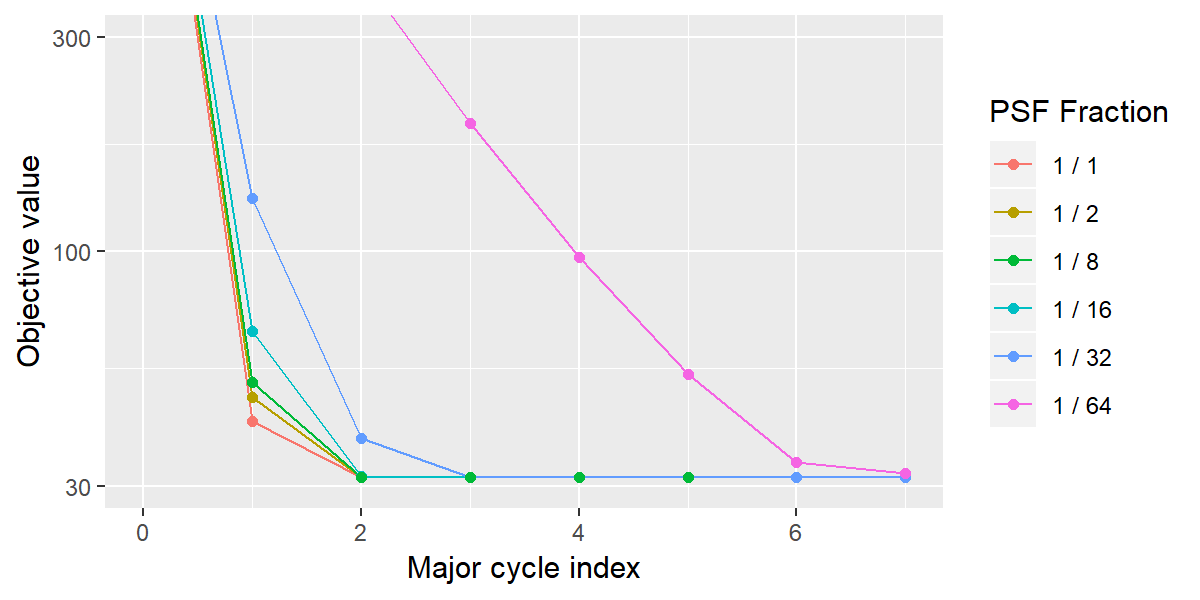
\includegraphics[width=\linewidth]{./chapters/10.results/gradient/ApproxDeconv/size.png}
	\end{subfigure}
	\begin{subfigure}[b]{0.195\linewidth}
		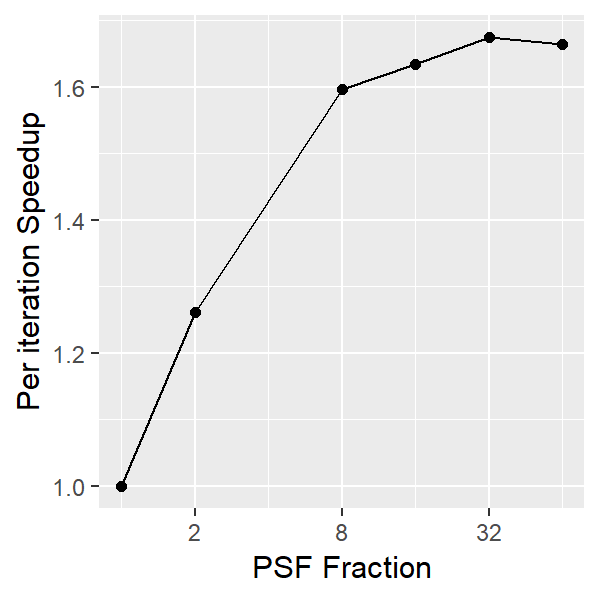
\includegraphics[width=\linewidth]{./chapters/10.results/gradient/ApproxDeconv/speedup_iter.png}
	\end{subfigure}
	\begin{subfigure}[b]{0.195\linewidth}
		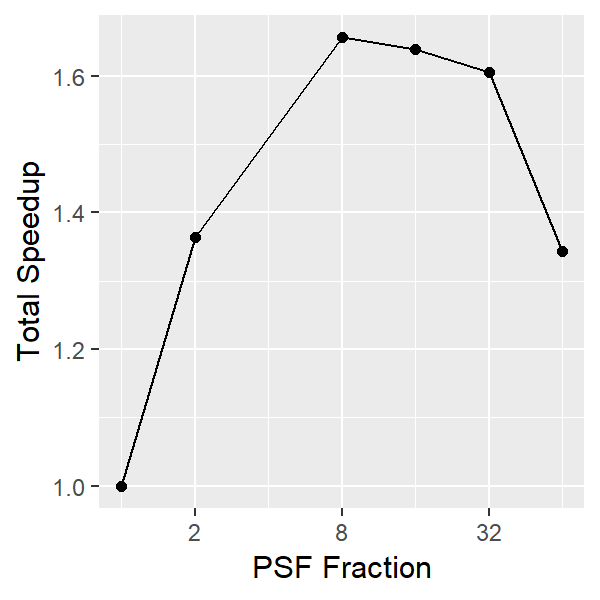
\includegraphics[width=\linewidth]{./chapters/10.results/gradient/ApproxDeconv/speedup_total.png}
	\end{subfigure}
	
	\caption{Convergence of the approximate deconvolution method.}
	\label{results:gradients:aproxDeconv}
\end{figure}

Again, the smallest window for which the serial coordinate descent algorithm converges is $\frac{1}{64}$. Similar to method 1, the serial coordinate descent algorithm reaches a similar objective value within 3 Major cycles, for all $PSF$ windows except $\frac{1}{64}$. The total speedup however is notably different: It reaches a larger total speedup. The total speedup curve generally matches better with the 'per iteration speedup' curve. This suggests that the approximate deconvolution method does not require significantly more iterations to converge, even when we use a $PSF$ window of $\frac{1}{16}$. 

The approximate deconvolution method is not guaranteed to lead to the same result. Nevertheless, the true objective value of the results are practically identical in Figure \ref{results:gradients:aproxDeconv}. However, as we mentioned before, this approximation method systematically under-estimates the true pixel values. The pixel magnitude is important in the self-calibration regime \cite{offringa2017optimized}. Self-calibration uses intermediate results of the image reconstruction to improve the calibration. A systematic under-estimation of the pixel values leads to a bias in self-calibration.


\subsubsection{Combination of Method 1 and 2}\label{results:gradients:comparison}
The approximation method 2, approximate deconvolution, leads to a systematic under-estimation of the true pixel values. This is undesirable for a reconstruction algorithm. The obvious question is, how does the serial coordinate descent algorithm perform when we combine the two approximation methods: We start with method 2. When the algorithm converged, we switch to method 1 and correct the systematic error introduced by method 2. We compare the speedup we achieve by combining the two approximation methods in Table \ref{results:gradients:comparison:speedup}.

\begin{table}[h]
	\centering
	\begin{tabular}{ c | c ||c|c } 
		\hline
		Method & $PSF$ Fraction & Iteration Speedup & Total Speedup \\ \hline \hline
		Original & $\frac{1}{16}$ & 1.00 & 1.00 \\ 
		(Method 1) Approx. gradient update & $\frac{1}{16}$ & 1.66 & 1.55 \\ 
		(Method 2) Approx. deconvolution & $\frac{1}{16}$ & 1.67 & 1.68 \\ \hline
		Combined & $\frac{1}{16}$ & 1.69 & 1.68 \\ 
		\hline
	\end{tabular}

	\caption{Results when combining the two approximation methods}
	\label{results:gradients:comparison:speedup}
	
\end{table}

Combining the two approximation methods leads to a total speedup with a $PSF$ window of $\frac{1}{16}$. The combined approximation method achieves a larger speedup than method 1 or method 2 on the same $PSF$ window size. We suspect the error each approximation method introduces is uncorrelated. Meaning the error we introduce with approximation method 2 can be efficiently corrected with approximation method 1, which leads to a higher total speedup. In total, the serial coordinate descent algorithm with a combined $PSF$ approximation method converged within 1486 seconds, or $24$ minutes.

Although the serial coordinate descent algorithm can be sped-up with the $PSF$ approximation, it does not lead to an algorithm with a comparable wall-clock time to CLEAN or multi-scale CLEAN. The speedup it achieves per iteration is limited by synchronization overhead: The serial coordinate descent algorithm uses all available processors to update the gradient map. With our approximation method, the serial algorithm can update an increasingly smaller facet of the gradient map. If we use a $PSF$ window which is $\frac{1}{16}$ of the total $3072^2$ size, the serial coordinate descent updates $384^2$ elements of the gradient map in each iteration. Utilizing all processors effectively with ever smaller $PSF$s becomes difficult.


\subsection{$PSF$ approximation with parallel coordinate descent}\label{pcdm:results}
First, we test the effect of our $PSF$ approximation method on the parallel coordinate descent algorithm. We test the deconvolution with increasingly smaller windows around the center of the full $PSF$. We measure the wall-clock time of the asynchronous iterations with $\tau = 8$ processors. We measure the value of the objective function after a batch $8 * 1000$ asynchronous iterations.

Note that the tests in this section are performed using the parallel block coordinate descent algorithm. It is able to group pixels into blocks, and minimize several blocks in parallel in each iteration. But grouping pixels into blocks slowed down the performance of the parallel block coordinate algorithm. The results of these tests can be found in the attachments.

Figure \ref{pcdm:results:psf} shows the result of our parallel coordinate descent algorithm with different $PSF$ fractions, combined with the ESO and the total seconds needed to converge. The $y$-axis shows the objective value, and the $x$-axis shows the elapsed seconds. Note that the axis of the figure are logarithmic. The 'kinks' in the lines are due to either the Major or the 'Minor' cycle resetting the residuals (remember: we excluded the time spent in the gridder or FFT, and only measured the time a batch of $8 * 1000$ asynchronous iterations).

\begin{figure}[h]
	\centering
	\begin{subfigure}{0.6\linewidth}
		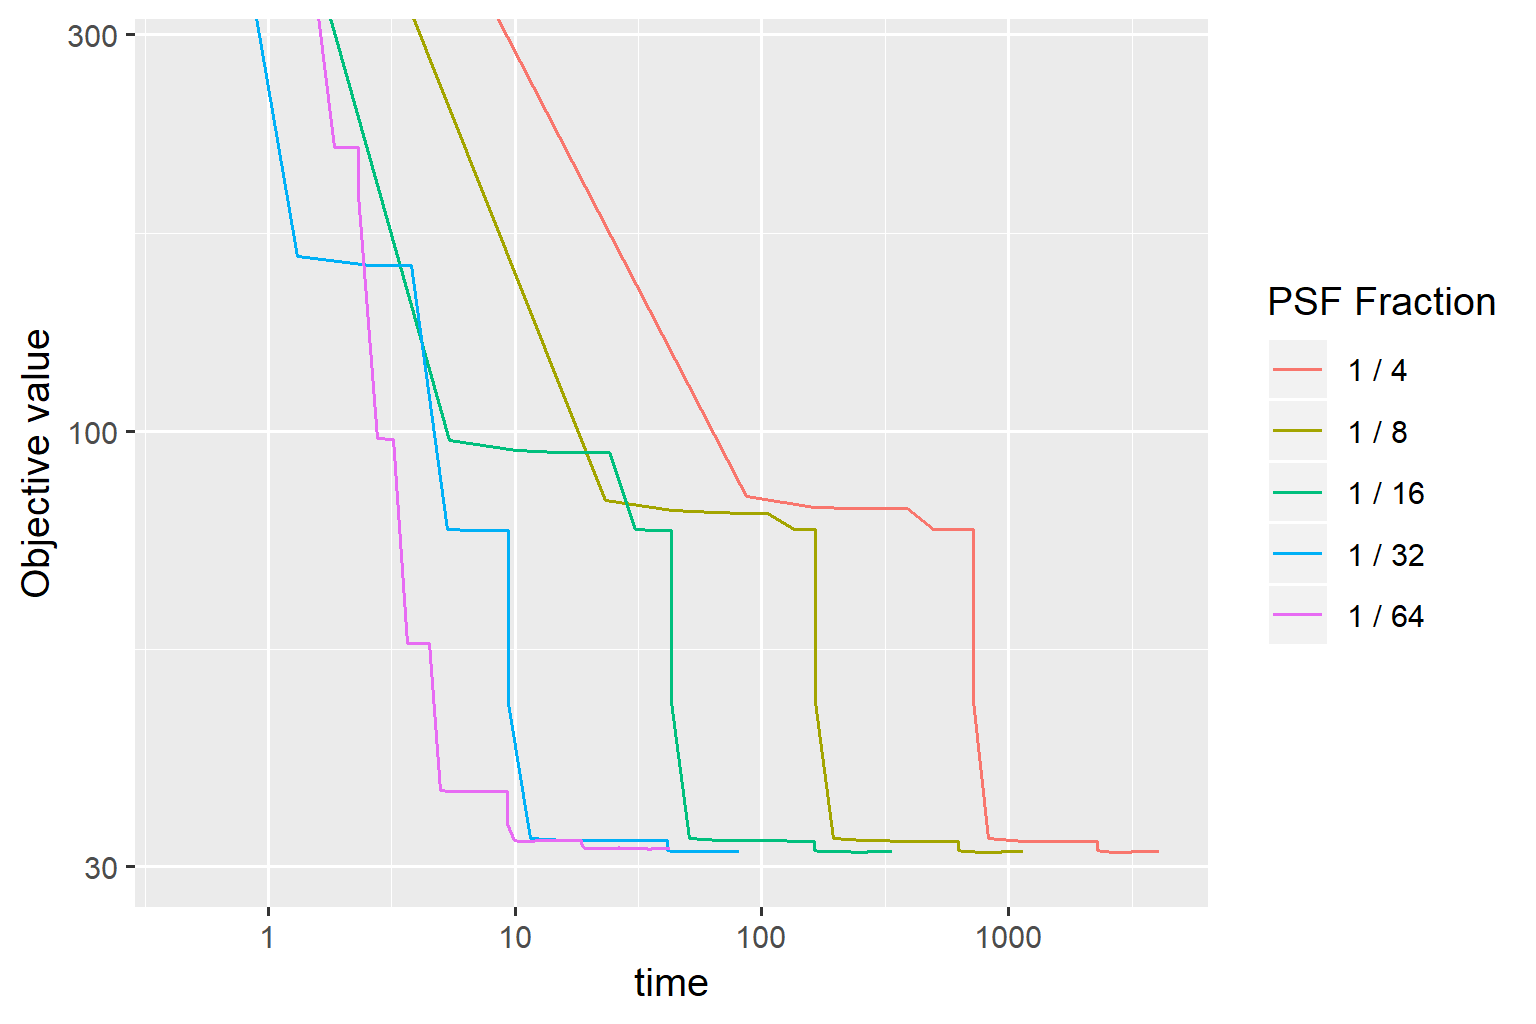
\includegraphics[width=1.0\linewidth]{./chapters/10.results/pcdm/psfSize.png}
	\end{subfigure}
	\begin{subfigure}{0.35\linewidth}
		\begin{tabular}{c | r | r}
			PSF & ESO & Total seconds \\ \hline
			1 / 4 & 2.750 & 4094 \\
			1 / 8 & 1.437 & 1148 \\
			1 / 16 & 1.109 & 339 \\
			1 / 32 & 1.027 & 81 \\
			1 / 64 & 1.001 & 42 \\
		\end{tabular}
	\end{subfigure}
	\caption{Convergence times with $PSF$ approximation}
	\label{pcdm:results:psf}
\end{figure}

Figure \ref{pcdm:results:psf} shows one line representing the value of the objective function after each batch of asynchronous iterations. Each line contains discontinuities. They either represent a Major cycle, or a 'Minor' cycle which was performed in-between the batch iterations. The wall-clock time of both the Major and 'Minor' cycle are excluded in this test. Clearly, the parallel coordinate descent algorithm benefits from our $PSF$ approximation method. If we use $\frac{1}{32}$ of the full $PSF$, the parallel coordinate descent algorithm spends a total of 81 seconds in to deconvolve the image. For comparison, the serial coordinate descent algorithm with $PSF$ approximation takes roughly 1400 seconds, or 23 minutes.

As expected, with increasing $PSF$ approximation, we get an ESO which is ever closer to 1. Remember: An ESO of 1 means that each processor in the parallel coordinate descent algorithm can have the same step size as the serial coordinate descent algorithm. With an approximation of $\frac{1}{32}$ and 8 parallel processors, the ESO is only marginally larger than 1.

Note that the speedup from fraction $\frac{1}{4}$ to $\frac{1}{8}$ is roughly a factor of $3.5$. The same holds true for the speedup of $\frac{1}{8}$ to $\frac{1}{16}$, and $\frac{1}{16}$ to $\frac{1}{32}$. The $PSF$ cutout from  $\frac{1}{8}$ to  $\frac{1}{16}$ results in four times fewer pixels. This suggests the speedup may be due to the reduced conflicts in the asynchronous update of the gradient map. With a smaller $PSF$ we reduce the change of several threads updating the same location in the gradient map, and we spend more time in the deconvolution itself.

For the rest of this project, we will use a $PSF$ approximation of $\frac{1}{32}$ for the parallel coordinate descent algorithm. The $\frac{1}{64}$ approximation is faster in this tests, but spends more time outside the asynchronous batch iterations (we excluded everything but the time spent in the asynchronous batch iterations) than with $\frac{1}{32}$.


\subsubsection{Pseudo-random strategy and the Search Factor}\label{pcdm:results:fraction}
As we discussed in Section \ref{pcdm:adaption}, a random pixel selection strategy seems to perform badly on the deconvolution problem. We created the pseudo-random strategy, which selects a pixel at random, but searches in it's neighborhood for the optimal pixel to optimize. It is a mixture between a random and a greedy selection strategy.

But the pseudo-random strategy introduces a new tuning parameter, which we call the 'Search Factor'. A Search Factor of 0 says that after a random pixel has been selected, we search 0\% of the neighboring pixels in the active set. It is identical to a pure random selection strategy. A Search Factor of 1.0 says that after a random pixel has been selected, we search 100\% of its neighbors in the image. For example, if we have 256 pixel with 8 threads, a search percentage of 1.0 selects a random pixel and looks at 32 pixel in its neighborhood. A search percentage of 100\% is identical to a greedy strategy, where each thread searches its partition of the entire image.

Our parallel coordinate descent algorithm needs a Search Factor larger than 0. We compare different Search Factors in Figure \ref{pcdm:results:search}.

\begin{figure}[h]
	\centering
	\begin{subfigure}{0.6\linewidth}
		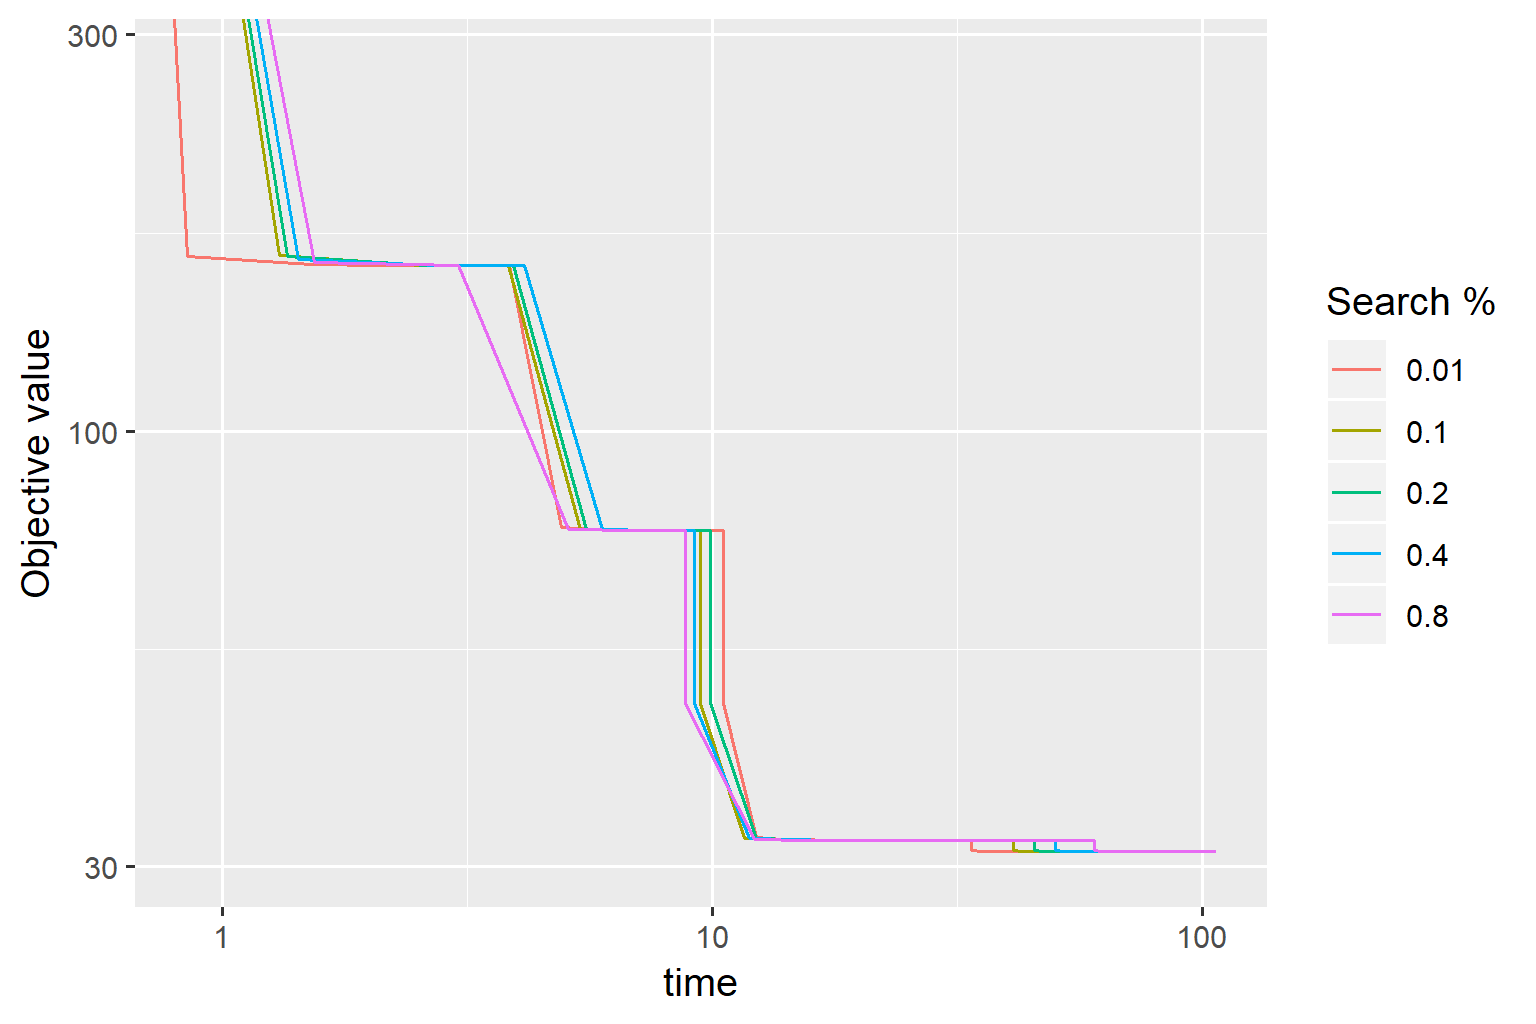
\includegraphics[width=1.0\linewidth]{./chapters/10.results/pcdm/searchPercent.png}
	\end{subfigure}
	\begin{subfigure}{0.35\linewidth}
		\begin{tabular}{c | r}
			Search Factor & Total seconds \\ \hline
			0.01 & 83 \\
			0.1 & 81 \\
			0.2 & 83 \\
			0.4 & 89 \\
			0.8 & 106 \\
		\end{tabular}
	\end{subfigure}
	\caption{Convergence times with different search percentages.}
	\label{pcdm:results:search}
\end{figure}

According to this test, the Search Factor tuning parameter influences the convergence speed, but tuning it does not lead to a significant speedup. A value between 0.01 and 0.4 leads to a similar wall-clock time. It is only when the parameter is set close to 1 (close to fully greedy) where we see a significant increase in wall-clock time.

The parallel coordinate descent algorithm is not deterministic. From each run to another, the algorithm selects different pixels at different points in time. This leads to an additional source of variance when measuring the total seconds to converge. In this project, we have not systematically tested the convergence time variance. The results presented in Figure \ref{pcdm:results:search} are from a single experiment run, where a Search Factor of $0.1$ lead to a slightly faster convergence time. This can change from experiment run to experiment run. At different runs had either the Search Factor $0.01$, $0.1$ or $0.2$ as the fastest.

We fixed the search percentage tuning parameter to a value of $0.1$ for all tests in this project. Based on this test, it does not have a significant influence on the convergence time, if the Search Factor is chosen small enough. It was enough to alleviate the problems a pure random strategy introduces in the deconvolution problem (discussed previously in Section \ref{pcdm:adaption}). However, we do not know whether this parameter generally has a small influence on convergence speed, or if it is merely due to the LMC observation we used for this project. To answer this question, we need further tests on different observations.


\subsection{Comparison to the serial coordinate descent algorithm}
In the previous section, we tested the convergence speeds of the parallel (block) coordinate descent algorithm with different tuning parameters. We showed how it achieves significant speedup with our $PSF$ approximation scheme, and showed the influence of the Search Factor tuning parameter. We excluded the negative tests: Grouping pixels into blocks did not lead to a faster convergence time. Also, using gradient acceleration \cite{fercoq2015accelerated} did not result in faster convergence times. These tests can be found in the attachments.

In this section, we compare the serial coordinate descent algorithm with the final, simplified parallel coordinate descent algorithm. We took the lessons from the previous tests and implemented a simplified parallel coordinate descent algorithm. It does not use gradient acceleration, and cannot group pixels into blocks. Each thread can only minimize a single pixel in parallel in each iteration. As we will see shortly, the simplified parallel coordinate descent implementation is faster than the previous implementation.

In this test, we compare the total wall-clock time spent on the deconvolution algorithm. Previously, we only measured the time spend in a batch of asynchronous iterations. This test also includes the time spent on auxiliary tasks in the deconvolution algorithm, and only excludes the time spent in the Major cycle.

We use the same hardware as in the tests of Section \ref{results:LMC}. The table \ref{pcdm:comp:table} shows the comparison between the serial and parallel coordinate descent algorithm. The parallel coordinate descent algorithm achieved a speedup factor of roughly $20$. While the serial coordinate descent algorithm takes over 20 minutes to deconvolve the image, the parallel coordinate descent algorithm takes less than two minutes in total.
%hardware

\begin{table} [h]
	\centering
	\begin{tabular}{c | c | r | r | c}
		Algorithm &  $PSF$  & Major Cycles & Total Seconds in Deconvolution & Speedup factor\\ \hline
		Serial CD & $\frac{1}{16}$ & 4 & 1486 & --\\
		Parallel CD & $\frac{1}{32}$ & 5 & 75 & $\approx 20$ \\
	\end{tabular}
	\caption{Speedup comparison of the serial and parallel coordinate descent algorithm. Both algorithms were compared on an Intel Xeon E3-1505M with 8 logical cores.}
	\label{pcdm:comp:table}
\end{table}

This parallel coordinate descent implementation is even faster than the implementation tested in the previous Section \ref{pcdm:results}. This implementation is simpler because it does not account for different block sizes. Each processor deconvolves a single pixel in parallel. The simplification leads to another decrease in wall-clock time.

The total deconvolution time of the parallel coordinate descent algorithm is in the range of the CLEAN algorithm. An exact comparison was not possible in this project. We did not implement the CLEAN algorithm in our .Net Core pipeline. However, the serial coordinate descent algorithm has an almost identical structure to the standard CLEAN algorithm, and we use this fact to get a rough comparison to CLEAN: The multi-scale CLEAN algorithm required 15'000 iterations to converge on the LMC observation. 15'000 serial coordinate descent iterations on the same hardware take approximately 230 seconds, which is about three times more than the parallel coordinate descent algorithm .

The serial coordinate descent algorithm is significantly slower than the parallel algorithm. However, it requires one major cycle less than the parallel algorithm to arrive at a similar reconstruction. The Figure \ref{pcdm:comparison:figure} compares the reconstruction of the two algorithms of the LMC observation.

\begin{figure}[h]
	\centering
	\begin{subfigure}{0.3\linewidth}
		\centering
		Serial CD + PSF approx
		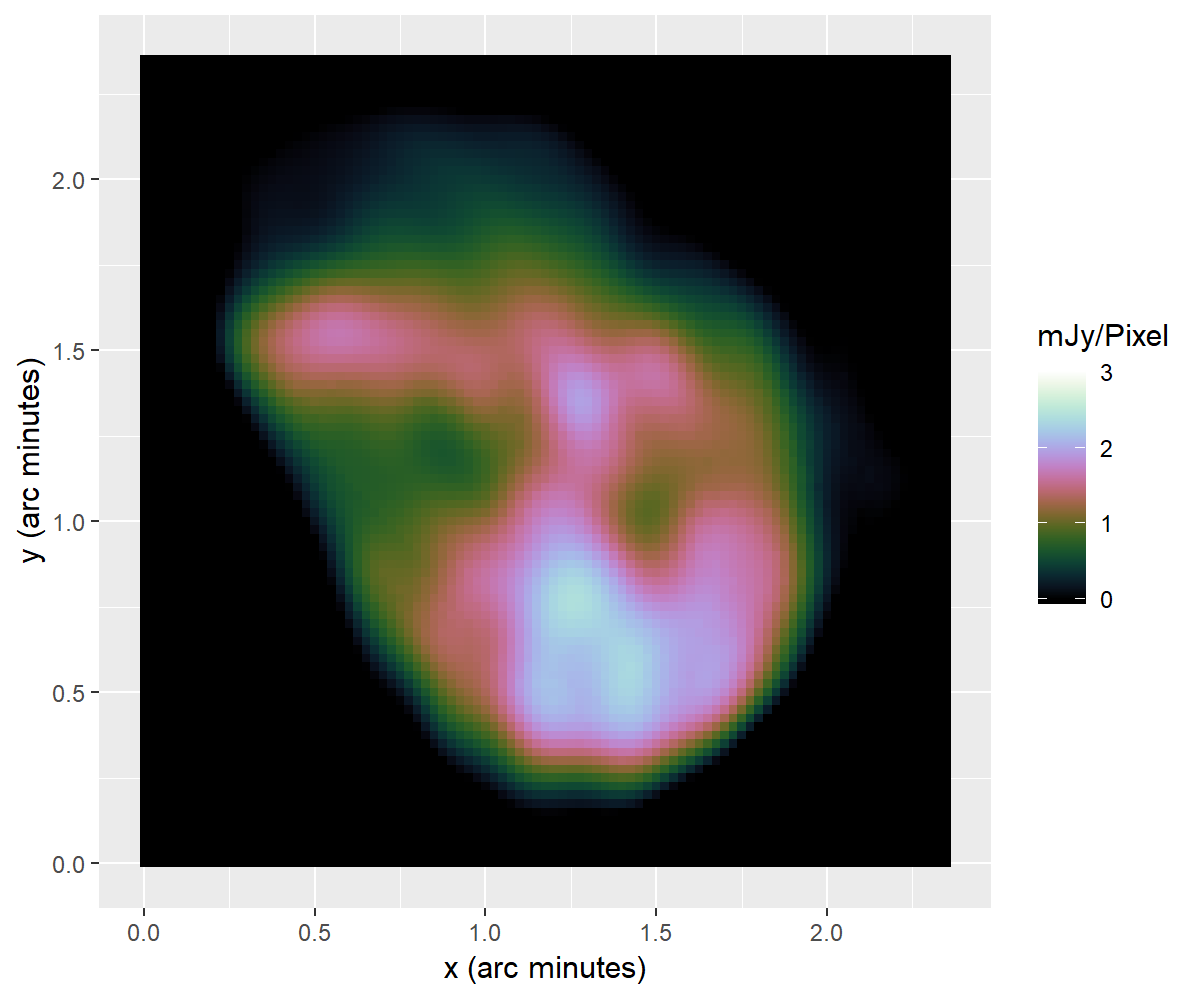
\includegraphics[width=1.0\linewidth]{./chapters/10.results/pcdm/SerialCD-N132.png}
		\\
		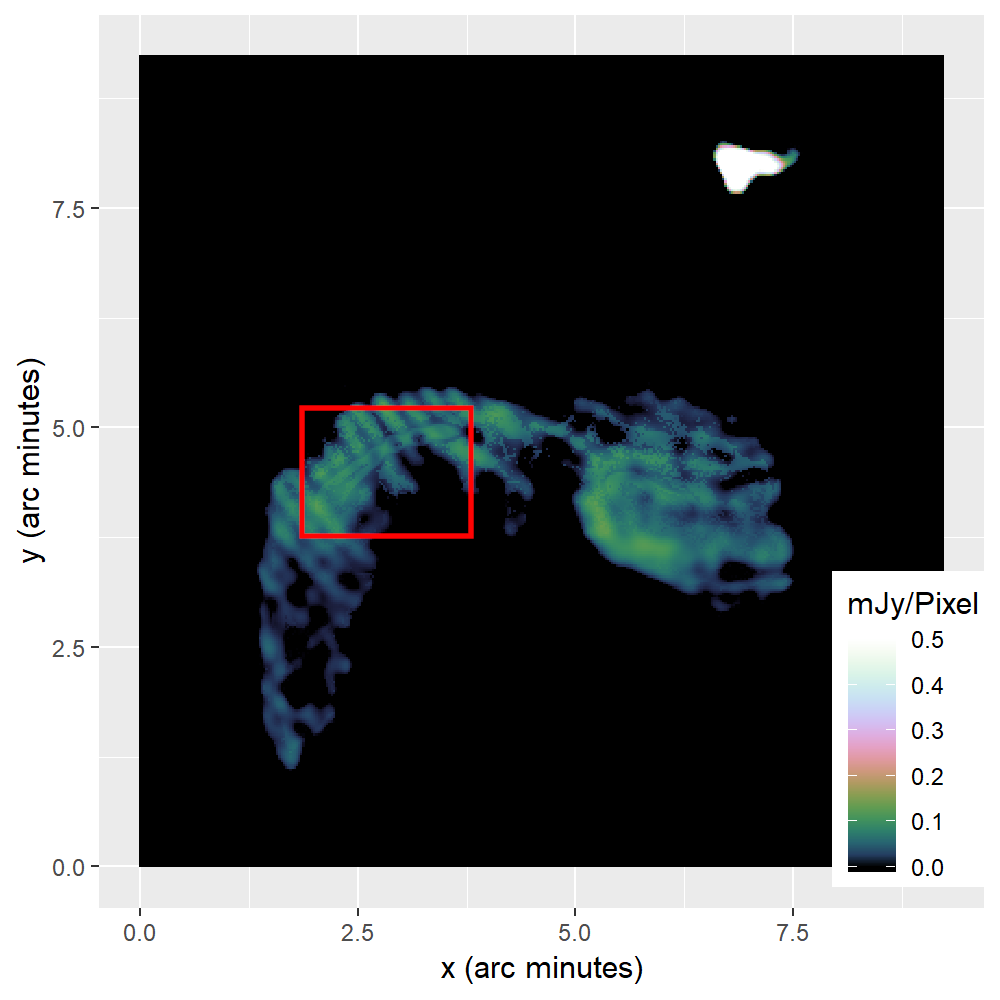
\includegraphics[width=1.0\linewidth]{./chapters/10.results/pcdm/SerialCD-Calibration-rec.png}
	\end{subfigure}
	\begin{subfigure}{0.3\linewidth}
		\centering
		Parallel CD + PSF approx
		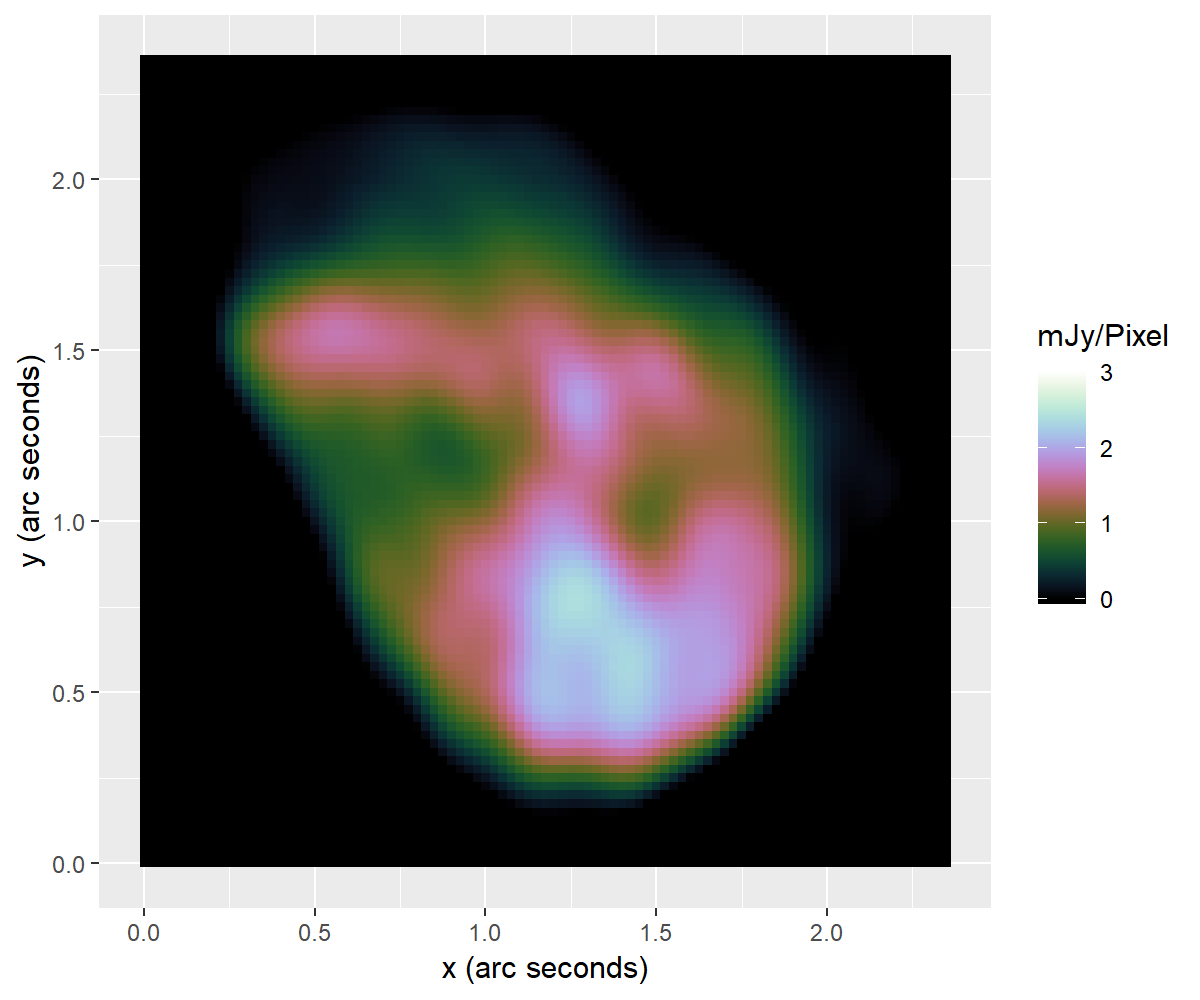
\includegraphics[width=1.0\linewidth]{./chapters/10.results/pcdm/PCDM-N132.png}
		\\
		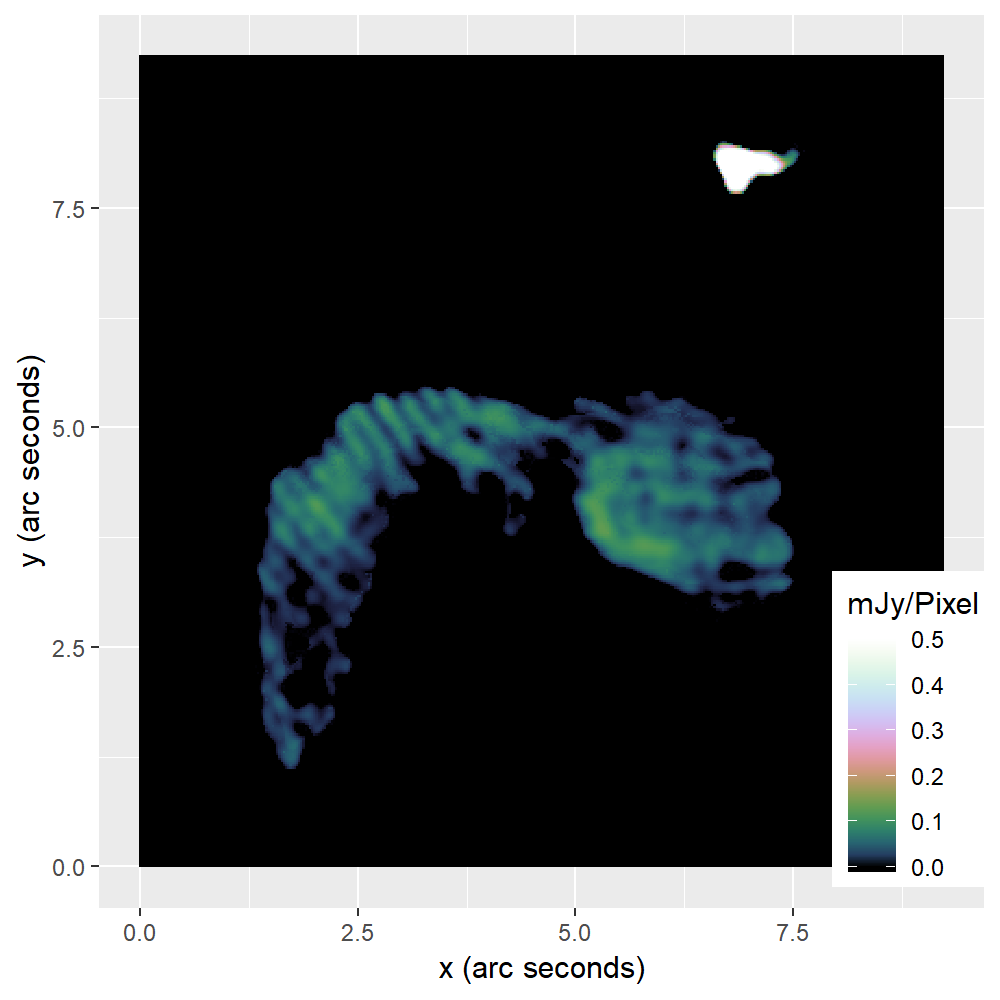
\includegraphics[width=1.0\linewidth]{./chapters/10.results/pcdm/PCDM-Calibration.png}
	\end{subfigure}
	\begin{subfigure}{0.3\linewidth}
		\centering
		Serial CD
		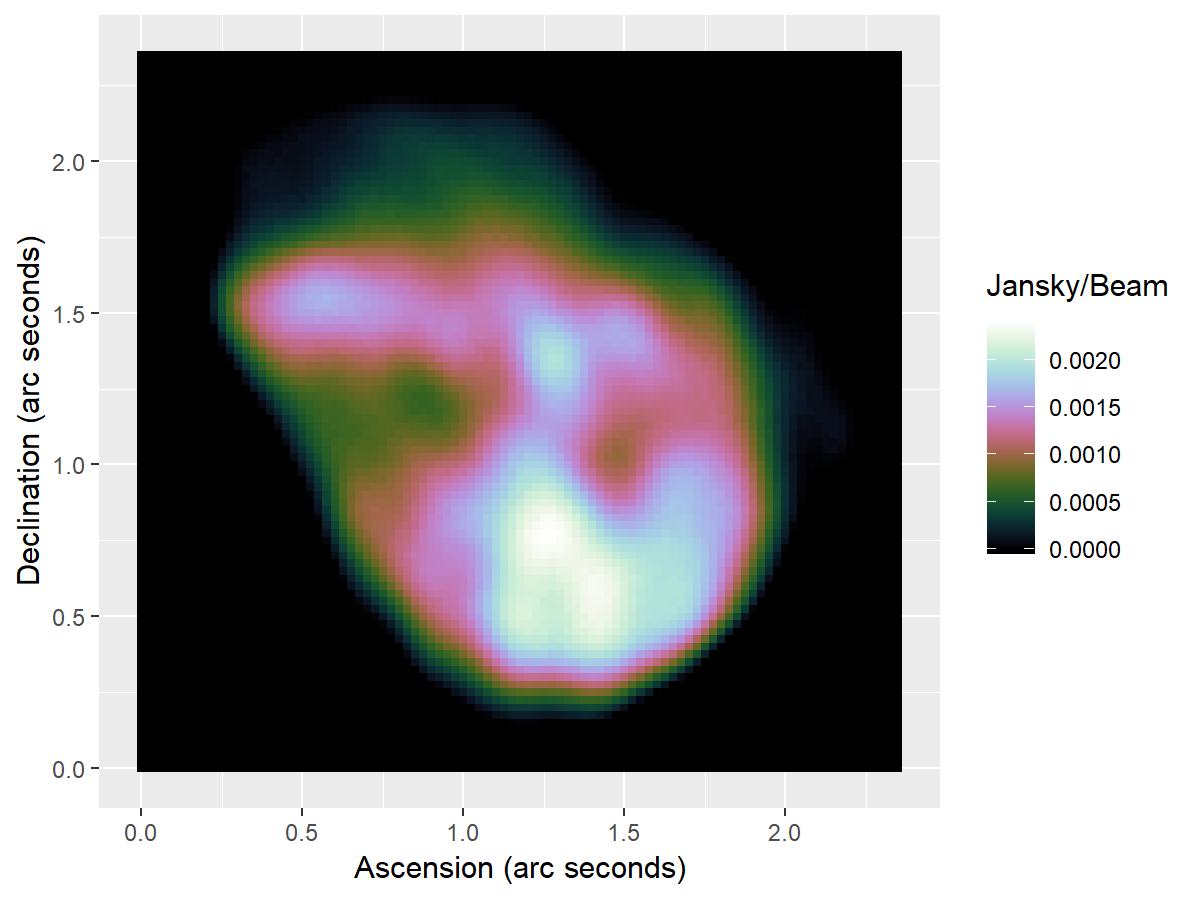
\includegraphics[width=1.0\linewidth]{./chapters/10.results/SerialCD/CD-N132.png}
		\\
		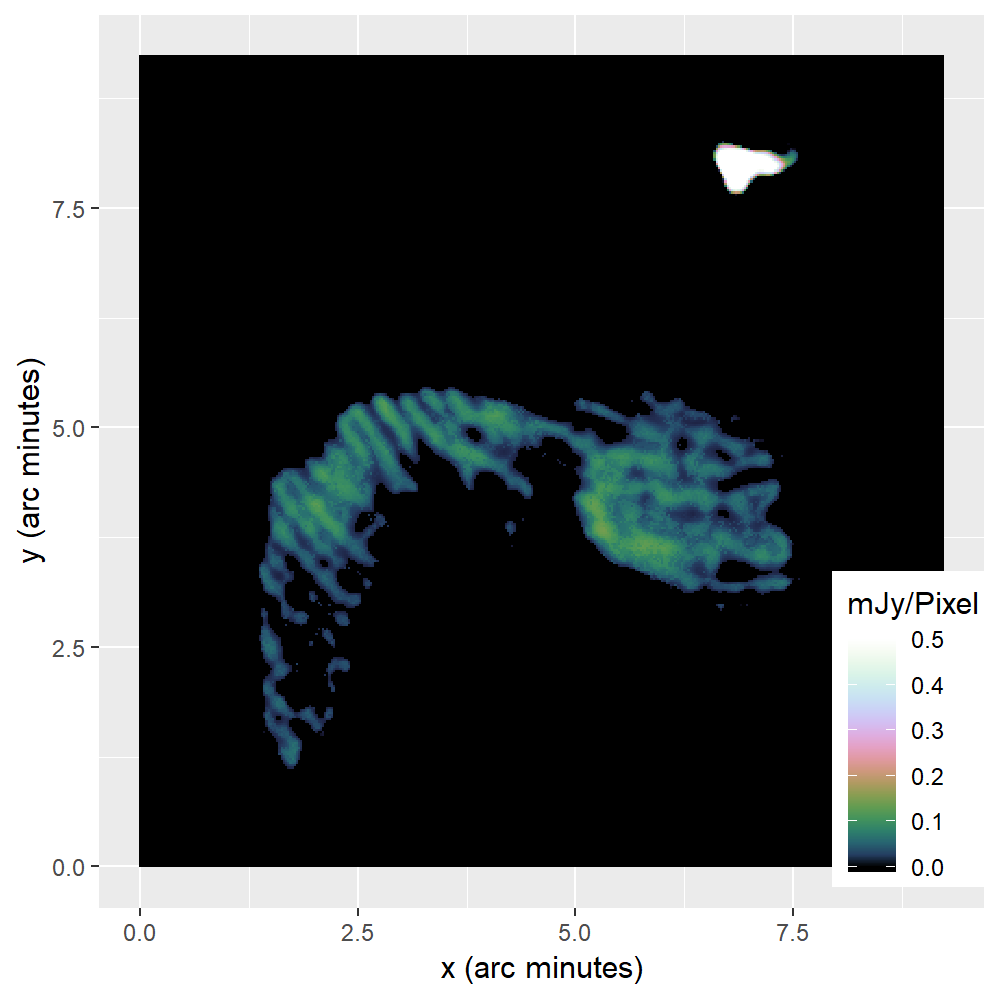
\includegraphics[width=1.0\linewidth]{./chapters/10.results/pcdm/CD-Calibration-Comp.png}
	\end{subfigure}
	
	\caption{Comparison of the serial and parallel coordinate descent reconstruction of the LMC observation.}
	\label{pcdm:comparison:figure}
\end{figure}

Both algorithms arrive at the same reconstruction. Both can super-resolve the N132D supernova-remnant, and have artifacts due to calibration errors. But the serial coordinate descent algorithm has left artifacts from the previous major cycles in the reconstruction: The red rectangle highlights a structure, which was added in a previous major cycle with the implicit path regularization. In a previous major cycle, only the highlighted structure was added. The next major cycle then added all the surrounding structure, including the "waves" from the calibration error. But the serial coordinate descent algorithm did not have enough iterations to properly integrate the old structure from the previous major cycle, leaving a "ghost" structure behind.

The serial coordinate descent can correct the artifact, but it either needs more iterations, or even another major cycle. In either case the serial coordinate descent algorithm needs more computing resources.

The parallel coordinate descent algorithm on the other hand does not contain the "ghost" structure. In a previous major cycle, the parallel algorithm has added a similar structure, but it was able to properly integrate it in the final reconstruction. We suspect this difference is due to the different number of pixels minimized: The reconstruction of the parallel algorithm is the result of roughly half a million single pixel minimizations, while the serial algorithm had performed roughly hundred thousand single pixel minimizations. The parallel algorithm had more iterations to integrate the structures detected from previous cycles.

Overall the reconstruction of the serial and parallel coordinate descent algorithms are similar. On the LMC dataset, the parallel algorithm was able to reconstruct a slightly superior reconstruction within a fraction of the total run time of the serial algorithm.


\subsection{Scalability of the parallel coordinate descent algorithm}\label{pcdm:scale}
The parallel coordinate descent algorithm out-performs the serial algorithm significantly on personal computing hardware. Lastly, we want to investigate how the parallel algorithm behaves when we increase the number of asynchronous processors.

Our parallel coordinate descent algorithm is based on PCDM\cite{richtarik2016parallel}. PCDM has been extended for the distributed setting as Hydra\cite{richtarik2016distributed}, and in its accelerated variant as Hydra$^2$\cite{fercoq2014fast}. Extending our parallel coordinate descent algorithm to the distributed setting was not possible in the time frame of this project. But if the parallel algorithm should be distributed in the future, we can apply the methods developed for Hydra and Hydra$^2$.

We test the parallel coordinate descent algorithm on a shared memory system (all processors have access to the same main memory), and test how the algorithm behaves for larger number of processors. Figure \ref{pcdm:scalability:proc} shows the results. The first graph shows the total speedup, the second plot shows the total number of iterations needed, and the last plot shows the ESO for increasing number of processors.

\begin{figure}
	\centering
	\begin{subfigure}{0.30\linewidth}
		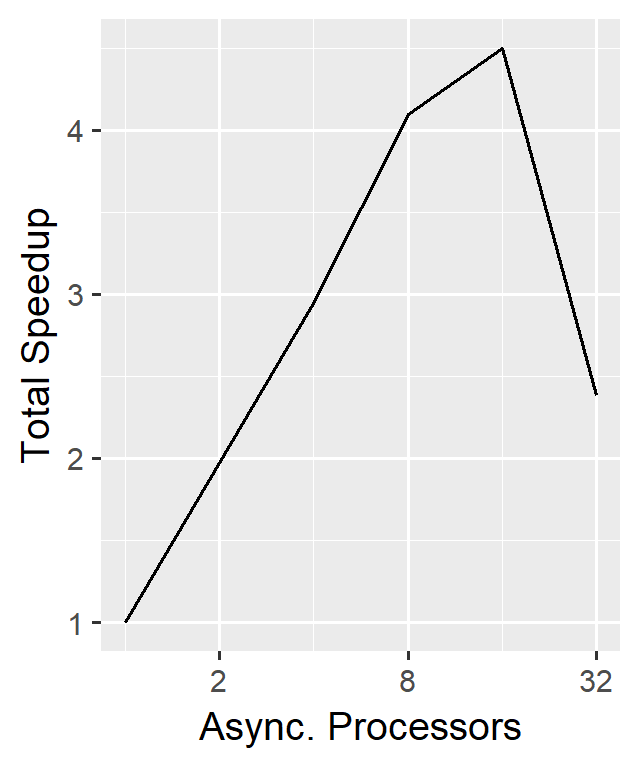
\includegraphics[width=1.0\linewidth]{./chapters/05.pcdm/scalability/speedup_pcdm_time.png}
	\end{subfigure}
	\begin{subfigure}{0.30\linewidth}
		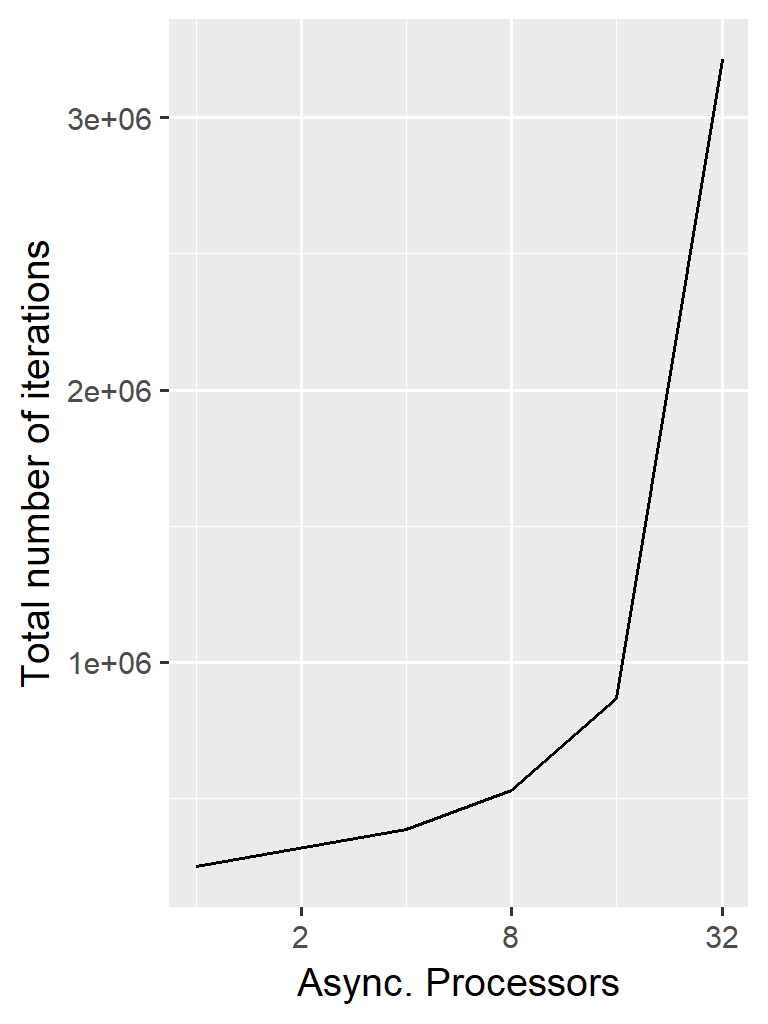
\includegraphics[width=1.0\linewidth]{./chapters/05.pcdm/scalability/speedup_pcdm_iter.png}
	\end{subfigure}
	\begin{subfigure}{0.30\linewidth}
		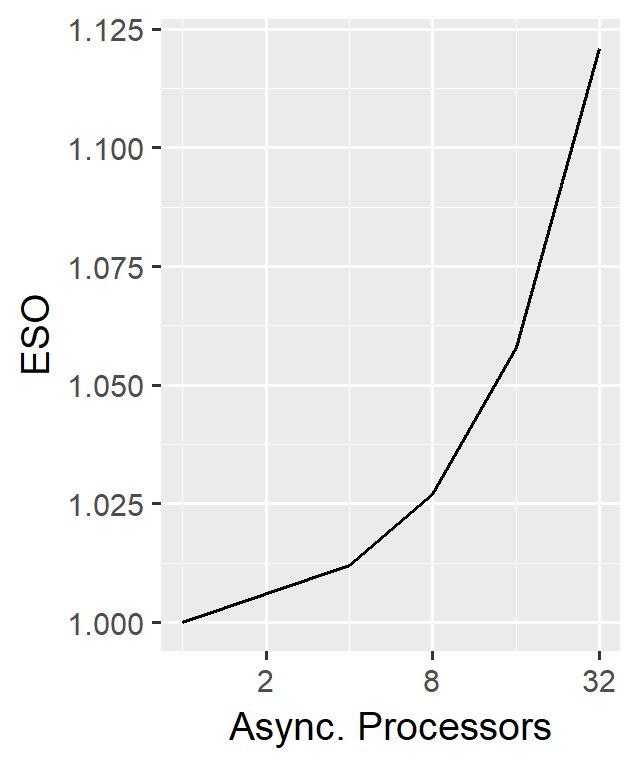
\includegraphics[width=1.0\linewidth]{./chapters/05.pcdm/scalability/speedup_pcdm_eso.png}
	\end{subfigure}
	\caption{Speedup comparison with increasing number of asynchronous processors.}
	\label{pcdm:scalability:proc}
\end{figure}

We see a linear speedup up to 8 processors. But afterwards, the speedup we receive diminishes quickly. After 16 processors, the parallel coordinate descent algorithm even becomes slower when more processors are added. The reason for this behavior lies in the total number of iterations the parallel algorithm needs to reconstruct a solution. As we see in Figure \ref{pcdm:scalability:proc}, it needs over 3 million parallel iterations to converge with 32 asynchronous processors. With 8 processors, it needs about half a million iterations to converge.

This drastic increase in total iterations quickly diminishes the speedup we receive by adding more asynchronous processors. This is partly due to the increase in the ESO: Adding more asynchronous processors increases the ESO, which in turn reduces the step size by which we can minimize a pixel in each iteration. However, we suspect there are more effects at play than just the ESO. The ESO for the number of processors is also shown in Figure \ref{pcdm:scalability:proc} does not increase as drastic as the total number of iterations needed. 

\begin{table} [h]
	\centering
	\begin{tabular}{c | r }
		Processors & Iterations per second \\ \hline
		1 & 1061.7 \\
		4 & 3849.7 \\
		8 & 9254.9 \\
		16 & 16'721.9 \\
		32 & 32'794.6 \\
	\end{tabular}
	\caption{Throughput of the parallel coordinate descent algorithms with additional processors.}
	\label{pcdm:scalability:throughput}
\end{table}

When we look at the throughput of the parallel coordinate descent algorithm in table \ref{pcdm:scalability:throughput}, we see that the number of iterations per second still increases roughly linearly with the number of asynchronous processors. If the parallel algorithm gets slowed down because of communication costs between processors (for example: multiple compare-exchange operations on the same entry in the gradient map), we would see a less-than-linear increase in throughput per added processor. Meaning the slowdown we see in Figure \ref{pcdm:scalability:proc} is likely not due to communication costs, but due to the drastic increase in total number of iterations.

Remember that the parallel coordinate descent algorithm runs a batch of asynchronous deconvolutions: Each asynchronous processor chooses pixels from the image for a given number of iterations, independently of the other processors. When we measure the absolute maximum pixel difference (the maximum step a serial greedy coordinate descent algorithm can take in one iteration) for 8 processors, we observe that it steadily decreases from one active set iteration to the next. At 32 processors, the absolute maximum pixel difference fluctuates from one batch of asynchronous iterations to the next.

This observation leads us to the ESO and our pseudo-random selection strategy: We may see the fluctuation, because we do not choose pixels uniformly at random, and their $PSF$s overlap more than we estimated with the ESO. In that case, the algorithm is in the danger of diverging, which would explain the fluctuation. The solution in that case would be to increase the ESO.

On the other hand, this fluctuation can also be observed with a proper random selection strategy. The second explanation is that with increasing number of processors, a single processor is simply too close to a random selection strategy. Remember: Our pseudo-random strategy greedily searches a fraction of the image. With an image of 1024 entries, 32 processors and a Search Factor of 0.1, each processor searches 10\% of $\frac{1024}{32}$ of the image. By adding more processors, each processor searches through fewer entries, although the total number of entries searched stays the same. By adding addtional processors, each single processor acts more according to a random selection strategy. The solution in that case would be to increase the Search Factor tuning parameter.

We tested these two explanations: We ran the parallel coordinate descent algorithm once with an increased ESO (the ESO which arises from 64 processors) and once with an increased Search Factor. The results are summarized in Table \ref{pcdm:scalability:table}.

\begin{table} [h]
	\centering
	\begin{tabular}{c | r | r | r | r | r | c}
		Test & Processors &  ESO & Search Factor & \# Iterations & Total Seconds & Speedup\\ \hline \hline
		Standard & 16 & 1.058 & 0.1 &  868k & 51 & 4.5\\\hline
		Standard & 32 & 1.121 & 0.1 & 3'213k & 98 & 2.4\\
		Larger ESO & 32 &  1.246 & 0.1 & 4'220k & 130 & 1.8 \\
		Larger Search & 32 &  1.121 & 0.4 & 1'171k & 47 & \textbf{5.0} \\
	\end{tabular}
	\caption{Speedup comparison for the parallel coordinate descent algorithm, once with increased ESO and once with increased Search Factor.}
	\label{pcdm:scalability:table}
\end{table}

Increasing the Search Factor lead to a significant decrease in total iterations, which in turn leads to a significant decrease in the wall-clock time, leading to a speedup factor of 5. With a larger Search Factor, the parallel coordinate descent algorithm is faster with 32 processors than with 16, and we removed the 'dip' in Figure \ref{pcdm:scalability:proc}. Noteworthy is that increasing the ESO in our parallel algorithm again lead to an increase in total number of iterations. This result suggests the ESO was not too low, and was not at fault for the slowdown we measured in Figure \ref{pcdm:scalability:proc}.

Nevertheless, these results are still surprising to us. As we mentioned before, whether we use 1 processor or 16 in our parallel coordinate descent algorithm, we still search the same number of pixels in the image. For a Search Factor of $0.1$, the algorithm always searches 10\% for every parallel iteration. Adding more processors simply reduces the number of pixels each processor checks. The results from Table \ref{pcdm:scalability:table} suggests that each processor in our parallel algorithm has to search through a minimum number of pixels in the image to run efficiently. But this view does not agree with our results from Figure \ref{pcdm:results:search}, where we used 8 processors and a Search Factor of 0.01. Each of the 8 processors searched through fewer pixels than in this test with 32 processors and a Search Factor of 0.1. But with 8 processors, it did not lead to a large increase in wall-clock time.

It is not clear why exactly our parallel coordinate descent algorithm needs so many more iterations to converge with 32 processors, or why increasing the Search Factor can remedy the problem. But the total number of iterations needed to converge seem to be the bottleneck for this algorithm. A thorough analysis may lead to a variant of our algorithm which needs fewer iterations to converge and therefore may be even faster. In the time frame of this project, it was not possible to further analyze the behavior.
